\documentclass[defaultstyle,10pt,master,Helvetica]{01.thesis}

\usepackage[T1]{fontenc}
\usepackage{titlesec, blindtext, color}
%% Packages
\typeout{}
\typeout{--------------------------------------------------------------}
\typeout{ +---+ Thesis Template                            }
\typeout{ +---+      Version 2.0, August 2011                         }
\typeout{ +---+  for Instituto Superior Tecnico (IST),                 }
\typeout{ +---+  Universidade Técnica de Lisboa                         }
\typeout{ * Using Thesis Style from Pedro Tomás                                }
\typeout{ * Created to write Dissertations                             }
\typeout{ * Conforms with IST Master Degree format and with most important packages setup        }
\typeout{ * Should conform with IST PhD Degree format (not verified)   }
\typeout{                                                              }
\typeout{ AUTHOR: Miguel Amador and João Marques                                          }
\typeout{                                                              }
\typeout{Important: Use all files in the archive, since this is based in all them. Modify dummy files at wish.                                                              }
\typeout{--------------------------------------------------------------}
\typeout{}

% Defines an additional alphabet... not required in most cases
% ------------------------------------------------------------
% \DeclareMathAlphabet{\mathpzc}{OT1}{pzc}{m}{it}

% PACKAGE babel:
% ---------------
% The 'babel' package may correct some hyphenisation issues of latex. 
% However in most situations it is not required.
\usepackage[english,portuguese]{babel}


% PACKAGE fontenc:
% -----------------
% chooses T1-fonts and allows correct automatic hyphenation.
%\usepackage[T1]{fontenc}
%\usepackage[latin1]{inputenc}
\usepackage[utf8]{inputenc}
%\usepackage{lmodern}

% Package ulem.
\usepackage{ulem} % Allows the use of other text emphatizer commands
\normalem %defines \emph{} to italic, instead of underline. 
\raggedbottom %declaration makes all pages the height of the text on that page. No extra vertical space is added. The \flushbottom declaration makes all text pages the same height, adding extra vertical space when necessary to fill out the page.

% PACKAGE date time:
% -----------------
% Lets you alter the format of the date that \today returns.
\usepackage{datetime}
\newdateformat{todaythesis}{%
\monthname[\THEMONTH]  \THEYEAR}

% PACKAGE latexsym:
% -----------------
% Defines additional latex symbols. May be required for thesis with many math symbols.
\usepackage{latexsym}

% PACKAGE amsmath, amsthm, amssymb, amsfonts:
% -------------------------------------------
% This package is typically required. Among many other things it adds the possibility
% to put symbols in bold by using \boldsymbol (not \mathbf); defines additional 
% fonts and symbols; adds the \eqref command for citing equations. I prefer the style
% "(x.xx)" for referering to an equation than to use "equation x.xx".
\usepackage{amsmath, amsthm, amssymb, amsfonts, amsbsy}

% PACKAGE multirow, colortbl, longtable:
% ---------------------------------------
% These packages are most usefull for advanced tables. The first allows to join rows 
% throuhg the command \multirow which works similarly with the command \multicolumn
% The second package allows to color the table (both foreground and background)
% The third package is only required when tables extend beyond the length of one page;
% with compatibilities with the tabular environment. The last allow the definitions of landscape pages, allowing the use of a different orientation for wider graphics or tables. See package documentation to see the implementation.
\usepackage{multirow}
\usepackage{colortbl}
\usepackage{supertabular}
\usepackage{pdflscape}
% \usepackage{longtable}

% PACKAGE graphics, epsfig, subfigure, caption:
% ---------------------------------------------
% Packages for figures... well you will certainly need these packages, with the exception
% of the 'caption' package. This only allows to define extra caption options.
% Notice that subfigure allows to place figures within figures with its own caption. It
% should be avoided to create an eps file with subfigures. That will mean that you won't be 
% able to reference those subfigures. Instead create an EPS file (the only graphics format supported
% by latex) for each of the subfigures and then use the command \subfigure (see below).
\usepackage{graphics}
\usepackage{graphicx}
\usepackage{epsfig}
\usepackage[hang,small,bf]{subfigure}
%\usepackage[footnotesize,bf,center]{caption}
\usepackage{dcolumn}
\usepackage{bm}
\usepackage{booktabs}
\usepackage{rotating}
\usepackage{multirow}

\usepackage[font=small,labelfont=bf,textfont=normalfont]{caption}

% PACKAGE algorithmic, algorithm
% ------------------------------
% These packages are required if you need to describe an algorithm.
% \usepackage{algorithmic}
% \usepackage[chapter]{algorithm}

% PACKAGE natbib/cite
% -------------------
% The two packages are not compatible, and you should use one of the two. Notice however that the
% IEEE BiBTeX stylesheet is imcompatible with the natbib package. If using the IEEE format, use the 
% cite package instead
\usepackage[square,numbers,sort&compress]{natbib}
%\usepackage{cite}

% PACKAGE acronyum
% -----------------
% This package is most useful for acronyms. The package guarantees that all acronyms definitions are 
% given at the first usage. IMPORTANT: do not use acronyms in titles/captions; otherwise the definition 
% will appear on the table of contents.
\usepackage[printonlyused]{acronym}
\usepackage[titletoc,title,header]{appendix}
\usepackage[noauto]{chappg}

% PACKAGE extra_functions VER COMO DEVE SER
% -----------------
% My Personal package: defines the following commands:
% \fancychapter{chaptername) -> Prints a fancier chapter (you can also use the fancychapter package for this)
% \hline{width} -> use for a replacement of the \hline command
% \Mark1, \Mark2, \Mark3, ...
\usepackage{00.extra_functions}


% PACKAGE hyperref
% -----------------
% Set links for references and citations in document
% Some MiKTeX distributions have faulty PDF creators in which case this package will not work correctly
% Long live Linux :D
\usepackage[plainpages=false]{hyperref}
\hypersetup{
             colorlinks=false,
             citecolor=red,
             breaklinks=true,
             bookmarksnumbered=true,
             bookmarksopen=true,
             pdftitle={Thesis Title},
             pdfauthor={Author Name},
             pdfsubject={Master Thesis in Biomedical Engineering},
             pdfcreator={Document Creator Name},
             pdfkeywords={Template, Latex, Thesis}}
\usepackage{float}
%\usepackage[final]{00.listofsymbols}
\usepackage{00.symlist}

% Set paragraph counter to alphanumeric mode
\renewcommand{\theparagraph}{\Alph{paragraph}~--}

\newcommand{\figref}[1]{Figure \ref{#1}}
\newcommand{\equationref}[1]{Equation (\ref{#1})}
\newcommand{\tableref}[1]{Table (\ref{#1})}

\newcommand{\textreg}{$\textsuperscript{\textregistered}$}
%% Page formatting
\hoffset 0in
\voffset 0in

%Alternative set of page geometry
%\oddsidemargin 0.71cm
%\evensidemargin 0.04cm
%\marginparsep 0in
%\topmargin -0.25cm
%\textwidth 15cm
%\textheight 23.5cm

\usepackage[top=2.5cm, bottom=2.5cm, inner=2.9cm, outer=2.5cm]{geometry}

\usepackage{fancyhdr}
\pagestyle{fancy}
\renewcommand{\chaptermark}[1]{\markboth{\thechapter.\ #1}{}}
\renewcommand{\sectionmark}[1]{\markright{\thesection\ #1}}
\fancyhf{} 
%\fancyhead[LE]{\bfseries\nouppercase{\leftmark}}
%\fancyhead[RO]{\bfseries\nouppercase{\rightmark}}
\fancyfoot[LE,RO]{\bfseries\small\thepage}
\renewcommand{\headrulewidth}{0.0pt}
\renewcommand{\footrulewidth}{0.0pt}
\addtolength{\headheight}{2pt} % make space for the rule
\fancypagestyle{plain}{% Used in Chapter titles
   \fancyhead{} % get rid of headers
   \renewcommand{\headrulewidth}{0pt} % and the line
   \renewcommand{\footrulewidth}{0pt}
   \fancyfoot[LE,RO]{\bfseries\small\thepage}
}

\fancypagestyle{begin}{%
   \fancyhead{}
   \renewcommand{\headrulewidth}{0pt}
   \renewcommand{\footrulewidth}{0pt}
   \fancyfoot[LE,RO]{\bfseries\small\thepage}
}
\fancypagestyle{document}{%
	\fancyhf{} 
	\fancyhead[LE]{\bfseries\nouppercase{\leftmark}}
	\fancyhead[RO]{\bfseries\nouppercase{\rightmark}}
	\fancyfoot[LE,RO]{\bfseries\small\thepage}
	%\renewcommand{\headrulewidth}{0pt}
	%\renewcommand{\footrulewidth}{0pt}
	\addtolength{\headheight}{2pt} % make space for the rule
}
\fancypagestyle{documentsimple}{%
	\fancyhf{}
	\fancyfoot[LE,RO]{\bfseries\small\thepage}
	%\renewcommand{\headrulewidth}{0pt}
	%\renewcommand{\footrulewidth}{0pt}
	\addtolength{\headheight}{2pt} % make space for the rule
}
\setcounter{secnumdepth} {5}
\setcounter{tocdepth} {5}
\renewcommand{\thesubsubsection}{\thesubsection.\Alph{subsubsection}}

\renewcommand{\subfigtopskip}{0.3 cm}
\renewcommand{\subfigbottomskip}{0.2 cm}
\renewcommand{\subfigcapskip}{0.3 cm}
\renewcommand{\subfigcapmargin}{0.2 cm}

\graphicspath{{Figures/}}

%% NEW CHAPTER STYLE %%%
\usepackage[T1]{fontenc}
\usepackage{titlesec, blindtext, color}
\definecolor{gray75}{gray}{0.75}
\newcommand{\hsp}{\hspace{20pt}}
\titleformat{\chapter}[hang]{\Huge\bfseries}{\thechapter\hsp\textcolor{gray75}{|}\hsp}{0pt}{\Huge\bfseries}

\pgfplotsset{compat=1.12}
%-----------------------------------------------------------
%-----------------------------------------------------------


\begin{document}
%% Use Main document Language
\selectlanguage{english}
%% ------
\pagestyle{begin}
\setcounter{page}{1} \pagenumbering{Alph}

% Add PDF bookmark 
\pdfbookmark[0]{Title}{Title}

\thispagestyle{empty}
\begin{flushleft} ~\\ \vspace{-12mm} \hspace{-12mm}  \includegraphics[width=50mm]{Cover/istnewlogo} 
\vspace{10mm}
%~\\ \vspace{50mm} % gráficos
\\ \begin{center} 
\includegraphics[width=1\linewidth]{Cover/coverimage}  \end{center} % gráficos
 \vspace{5mm}
\centering
\LARGE \textbf{Thermographical analysis of interface heat transfer mechanisms, with high time precision}
%\\ \vspace{10mm}
%\Large Subtitle
\\ \vspace{15mm}
\Large \textbf{Pedro Daniel Fernandes Pontes} \\
\vspace{12mm}
\large Thesis to obtain the Master of Science Degree in
\\ \vspace{2mm}
\LARGE \textbf{Mechanical Engineering}
\\ \vspace{10mm}
\large Supervisor(s): Prof./Dr. Ana Sofia Oliveira Henriques Moita 
\\ \vspace{15mm}
\Large \textbf{Examination Committee}
\\ \vspace{5mm}
\large Chairperson:	Prof. Lorem \\
\large Supervisor: Prof. Lorem Ipsum\\
\large Co-Supervisor: Prof. Lorem Ipsum \\
\large Members of the Committe: Dr. Lorem Ipsum \\
Prof. Lorem Ipsum
 
\vspace{15mm}

%\Large \textbf{\todaythesis\today} \\
\Large \textbf{October 2016} \\
\let\thepage\relax
\end{flushleft}
\pagebreak


\clearpage
% Since I am using double sided pages, the second page should be white.
% Remember that when delivering the dissertation, IST requires for the cover to appear twice.

\thispagestyle{empty}
\cleardoublepage

\setcounter{page}{1} \pagenumbering{roman}

\baselineskip 18pt % line spacing: -12pt for single spacing
                   %               -18pt for 1 1/2 spacing
                   %               -24pt for double spacingnts} 
\thispagestyle{empty}
\pdfbookmark{Acknowledgments}{Acknowledgments}

\begin{acknowledgments} 

%First would like to thank IST for being my home and teaching me everything I needed to get this far. It has been truly amazing studying here and knowing so many inspiring teachers and so many brilliant colleagues.
\par - prof e ema
\par - co-workers
\par - friends
\par - family and fu
\par - outros?


\end{acknowledgments}

\hbox{} \vfill
\begin{flushright}
\small \textit{\textbf{"Try not to become a person of success, but rather try to become a person of value."}} %%% MUDAR %%%
\\ \vspace{2mm}  
\scriptsize Albert Einstein
\end{flushright}

\clearpage
\thispagestyle{empty}
\cleardoublepage
%\pdfbookmark{Acknowledgments}{Acknowledgments}
\begin{acknowledgments} 

I would like to thank the Academy, bla bla bla..

\end{acknowledgments}
\clearpage
\thispagestyle{empty}
\cleardoublepage
\selectlanguage{english}
\begin{abstract}

bla bla

\end{abstract}
\begin{keywords}
Keywords (English)
\end{keywords}
\clearpage
\thispagestyle{empty}
\cleardoublepage
\selectlanguage{portuguese}
\begin{resumo}

O objectivo deste trabalho ... (Português)

\end{resumo}
\begin{palavraschave}
Palavras-Chave (Português)
\end{palavraschave}
\clearpage
\thispagestyle{empty}
\cleardoublepage
%% Use Main document Language
\selectlanguage{english}
%% ------
% This is required for the fancy chapters
\dominitoc
\dominilof
\dominilot

%%%%%%%%%%%%%%%%%%%%%%%%%%%%%%%%%%%%%%%%%%%%%%%%%%%%%%%%%%%%%%%%%%%%%%
% List of contents
%\renewcommand{\baselinestretch}{1}
\pdfbookmark[0]{Index}{index}
\pdfbookmark[1]{Contents}{toc}
\tableofcontents
% \contentsline{chapter}{References}{\pageref{bib}}
\clearpage
\thispagestyle{empty}
\cleardoublepage
%\renewcommand{\baselinestretch}{1.5}
%%%%%%%%%%%%%%%%%%%%%%%%%%%%%%%%%%%%%%%%%%%%%%%%%%%%%%%%%%%%%%%%%%%%%%
% List of figures
\pdfbookmark[1]{List of Figures}{lof}
\listoffigures
\clearpage
\thispagestyle{empty}
\cleardoublepage

%%%%%%%%%%%%%%%%%%%%%%%%%%%%%%%%%%%%%%%%%%%%%%%%%%%%%%%%%%%%%%%%%%%%%%
% List of tables
\pdfbookmark[1]{List of Tables}{lot}
\listoftables
\clearpage
\thispagestyle{empty}
\cleardoublepage

% %%%%%%%%%%%%%%%%%%%%%%%%%%%%%%%%%%%%%%%%%%%%%%%%%%%%%%%%%%%%%%%%%%%%%%
% % List of algorithms
% Requires packages algorithmic, algorithm
% \pdfbookmark[1]{List of Algorithms}{loa}
% \listofalgorithms
% \cleardoublepage
\acresetall
%% Remain list of table titles are set manualy
% %%%%%%%%%%%%%%%%%%%%%%%%%%%%%%%%%%%%%%%%%%%%%%%%%%%%%%%%%%%%%%%%%%%%%%
 % List of acronyms
\pdfbookmark[1]{List of Acronyms}{loac}

\chapter*{Abbreviations}


% See more at http://staff.science.uva.nl/~polko/HOWTO/LATEX/acronym.html

\begin{acronym}
\acro{acro}{Dummy Acronym}
\end{acronym}

\clearpage
\thispagestyle{empty}
\cleardoublepage




%%%%%%%%%%%%%%%%%%%%%%%%%%%%%%%%%%%%%%%%%%%%%%%%%%%%%%%%%%%%%%%%%%%%%%
% List of symbols
\pdfbookmark[1]{List of Symbols}{los}

\listofsymbols

\clearpage
\thispagestyle{empty}

\cleardoublepage
% Pages number is starting now with arabic style... until now it was on roman mode
\pagenumbering{arabic} \setcounter{page}{1}
\baselineskip 18pt
%% Use Main document Language
\selectlanguage{english}
%% Define the title of Chapter Table of Contents
\mtcsettitle{minitoc}{Contents}
%% ------
\pagestyle{documentsimple}%Simple head
% %%%%%%%%%%%%%%%%%%%%%%%%%%%%%%%%%%%%%%%%%%%%%%%%%%%%%%%%%%%%%%%%%%%%%%
% The Introduction:
% %%%%%%%%%%%%%%%%%%%%%%%%%%%%%%%%%%%%%%%%%%%%%%%%%%%%%%%%%%%%%%%%%%%%%%
\chapter{Introduction}
\label{cap:int}

\section{Motivation}
\label{sec:int_motivation}

\par Heat transfer in fluid-solid interfaces, with fluid state change, is a common phenomena in the nature and technology. It is still a mystery, although getting smaller with time, what mechanisms transfer heat during boiling. Because there are countless applications in the industry where this phenomena occurs, there is a need to know what actually is happening so we can then improve these applications by more efficiently controlling them. \\
\par Surface heat removal using liquids is a complex and fast happening that often involves state change. So, to study this type of phenomena, we need high precision equipment with, not only high spatial precision, but also time precision. In this field of study, many types of measuring equipment have been used to quantify and qualify such phenomena. The use of a thermocouple, for instance, which is a really common method, can be intrusive to the measured process, can only measure one point and cannot be in contact with electricity. With this in mind, infra-red thermography has been a great alternative to some of the existing intrusive temperature measuring methods. A thermographical camera with a good calibration can give high precision temperature results at high frame rates, which can give high definition qualitatively and, more importantly, quantitatively accurate thermal images. The IR camera also outputs two dimensional images, a great advantage when trying to understand this kinds of processes. \\
\par Although the IR camera use will be centered in the boiling process, the heat transfer mechanisms in droplet surface impact will also be studied. Both require high precision results, so calibration and result processing should be studied with great care. \\
\par While this work is developed, a computational study by Emanuele Teodori is being made, and this work's results will also be used to validate the computational model in use.
\section{State of The Art}
\label{sec:int_state}

State of The Art Section.

\subsection{Dummy Subsection A}
\label{subsec:subsectiona}

State of Art Subsection A

\subsection{Dummy Subsection B}
\label{subsec:subsectionb}

State of Art Subsection B


\section{Objectives}
\label{sec:int_contributions}

\par The main objective of this dissertation is to optimize the use of the IR Camera to study interface phenomena in droplet impact. This not only includes improving studying the positioning of the camera and data processing, but also study the techniques that are involved in getting to the heat transfer in the various interfaces. The techniques used will be an adaptation of what previous authors did using thin foil surfaces, always trying to improve both the time and spatial resolution.\\

\par To achieve good quantitative results with the camera, it is of the most importance that this camera is properly calibrated, so another important objective will be create a process that can accurately calibrate a camera for the laboratory's use. To add to a good calibration it will be also very important to create quality IR data processing tools that can be used in future work.\\

\par One last objective will be to vary the experiments variables and analyze if the collected images react as expected to the variation. This setup will be tested with foils at under, during and over saturation temperature, with an elevated and lower droplet impact velocity, with different liquids and also different surface wettability. This will evaluate if the improvements to the existent method allowed better results.
\section{Thesis Outline}
\label{sec:int_outline}

\par In this work an introduction to the used concepts will be given. This will go through IR thermography, wettability and droplet impact physics and heat transfer phenomena. This introduction will be presented in Chapter 2.\\

\par In Chapter 3, the 2 conceived experimental setups will be explained. This will include explanation about the role of every material present in the setup and also the process of collecting data. The functioning of the IR Camera will be clarified aswell as the data collecting methods and software calibration options.\\

\par One of the most important parts of this work is the proposed calibration. In Chapter 4, the proposed calibration method will be explained and compared against the existing calibration. All the thought process behind the calibration and its construction will be shown. The data processing code that was made specially for this camera is also explained in this chapter and its effects shown.\\

\par The results of the experiments in various conditions will be presented in Chapter 5, along with the observed phenomena, making a bridge between the expected results, from the introductory chapter, and the obtained ones. The conclusions about these results and the used method will be discussed in Chapter 6 and clarified if the proposed objectives were reached. Also in this chapter, future work that will be developed around this method will be discussed.

\cleardoublepage
% %%%%%%%%%%%%%%%%%%%%%%%%%%%%%%%%%%%%%%%%%%%%%%%%%%%%%%%%%%%%%%%%%%%%%%
% Dummy Chapter:
% %%%%%%%%%%%%%%%%%%%%%%%%%%%%%%%%%%%%%%%%%%%%%%%%%%%%%%%%%%%%%%%%%%%%%%

% %%%%%%%%%%%%%%%%%%%%%%%%%%%%%%%%%%%%%%%%%%%%%%%%%%%%%%%%%%%%%%%%%%%%%%
% The Introduction:
% %%%%%%%%%%%%%%%%%%%%%%%%%%%%%%%%%%%%%%%%%%%%%%%%%%%%%%%%%%%%%%%%%%%%%%
\chapter{Theoretical Background}
\label{cap:theoretical}

\textit{In this chapter some theoretical background will be given about what's going to be discussed further.}

\section{Infrared Thermography}
\label{sec:sectiona}

Heat transfer through radiation is the way, in thermography, most often used to gather it's results and one of the main objects of study of this work is how to correctly transform the measured radiation intensity plus the information on the body emissivity and surrounding conditions in an accurate temperature estimate. To do so, some theoretical notions will have to be mentioned so that thermography can be better understood.

\subsection{Radiation Intensity to Temperature Conversion}
\label{subsec:rad2tem}

Radiation is emitted by all bodies at $T>0$. The intensity of this radiation largely depends on the direction, wavelength and of course temperatures. For example, above 500ºC, a body's radiation is almost entirely in the IR wavelength \cite{IRCAM}. Besides emitting radiation a body can also absorb ($\alpha$), reflect ($\rho$) and radiation can even pass through it ($\tau$). Adding all this elements we get the Total Radiation Law:
\begin{equation}
    W = W\alpha + W\rho + W\tau
\end{equation}
... in which $W$ represents the total energy transmitted through radiation. Using a simplified version we can also say that:
\begin{equation}\label{eq:1}
	1 = \alpha + \rho + \tau
\end{equation}
Note that in the equation \ref{eq:1}, $\alpha$, $\rho$ and $\tau$ represent their respective fractions of the incident radiation energy, and need to have values between 0 and 1.\\

\subsubsection{Blackbody Equations}

\par One of the most important concepts that is used in this work is the concept of \textit{blackbody}. A \textit{blackbody} is characterized for absorbing all energy transmitted through radiation. In the ideal case of a \textit{blackbody} the coefficients assume the following values: $\alpha=1, \ \rho=0, \ \tau=0$. The blackbody is also a perfect emitter. The emissivity ($\varepsilon$) of a body characterizes the efficiency of a body for emitting energy, so it's the ratio between energy emitted and the energy emitted if the body was a \textit{blackbody}. With this in mind we can use the equation \ref{eq:2} for a \textit{blackbody}. This equation is called Kirchhoff Law. Kirchhoff Law is also applied for the same wavelength ($\lambda$) so we can also use equation \ref{eq:3}.

\begin{equation}\label{eq:2}
\alpha=\varepsilon
\end{equation}
\begin{equation}\label{eq:3}
\alpha(\lambda)=\varepsilon(\lambda)
\end{equation}
\par For the specific case of a \textit{blackbody} we can also apply equation \ref{eq:4}. This equation is called Stefan-Boltzmann law and it states the relation between energy emitted through radiation and the temperature of the body. If the body is not perfectly black, but it's absorption/reflection/transparency properties don't vary with the wavelength, we call it a \textit{greybody} and can use equation \ref{eq:5}.
\begin{equation}\label{eq:4}
W=\sigma T^4
\end{equation}
\begin{equation}\label{eq:5}
W=\varepsilon \sigma T^4
\end{equation}
...where $\sigma=5.670373 \times 10^8 W m^{-2} K^{-4}$ and it's called the Stefan-Boltzmann constant.\\
\par It's fairly obvious these are concepts that illustrate ideal situations, and even though in most experiments shown further ahead the materials are chosen to be as close to \textit{black} or \textit{greybodies}, those aren't perfect. Of course this is attenuated by the fact that thermography measures in small intervals of wavelength. The next subsection will relate how does one choose a wavelength interval, and it's relation with the atmosphere.

\subsubsection{Atmosphere Attenuation}
\label{subsec:atmat}

\par The thing that separates almost every thermographical camera from its target is the atmosphere, which has good and bad transmittance in different wavelengths. The atmosphere attenuation comes with the complexity of it's composition. For example, each of the following molecules: $H_2O$, $O_2$, $CO_2$ have certain wavelength values for which $\tau=0$. This means that in these wavelengths IR radiation will not pass through the atmosphere and its intensity cannot be measured.\\
\par This issue calls for the necessity of choosing a wavelength \textit{window} for which the transmittance is close to 1. These \textit{windows} can be seen in Figure \ref{fig:atm}. It is possible to identify 2 main regions: the medium-wave \textit{window} (from 2-5 $m \mu$), or MW, and the long-wave \textit{window} (from 7.5-13.5 $m \mu$), or LW. The used camera works in the MW range so a selective range of wavelength inside it had to be chosen so to avoid bad atmosphere transmittance.

\begin{figure}
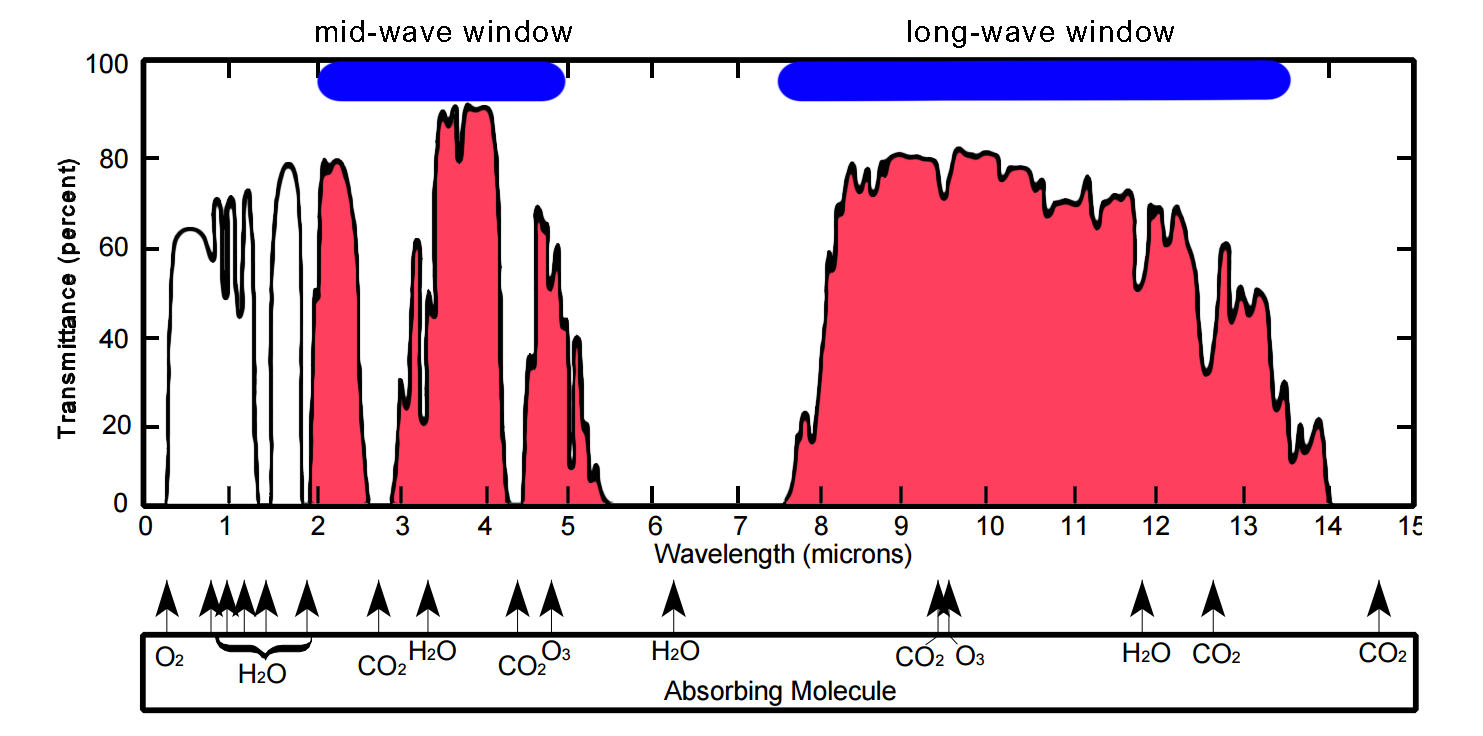
\includegraphics[width=1\linewidth]{Figures/2.Chapter/atmospheric_window.png}
\caption{Atmospheric Windows}
\source{Adaptation from chapter 7's Figure 10 of \cite{desk1997electronic}}
\label{fig:atm}
\end{figure}

\subsubsection{Total Radiation}
\par When measuring a body's temperature with the IR Camera, there are other radiation sources that have to be accounted for. In total we can divide these radiation sources in 3 categories, shown bellow wi:
\begin{itemize}
\item The radiation emitted by the object/objects of study
\begin{equation}
W_{obj}=\varepsilon_{obj} \ \sigma \ T_{obj}^4
\end{equation}
\item The radiation emitted by the atmosphere (where $ \ \varepsilon_{atm}=1-\tau_{atm}$ because $\rho_{atm}~=0$)
\begin{equation}
W_{atm}= (1-\tau_{atm}) \ \sigma \ T_{atm}^4
\end{equation}
\item The radiation from the surroundings reflected by the object/objects.
\end{itemize}
\begin{equation}
W_{refl}=(1-\varepsilon_{obj}) \ \sigma \ T_{refl}^4
\end{equation}
...where $T_{refl}$ refers to the apparent temperature of the surrounding that's radiating to the body.\\
\par Figure \ref{fig:camscheme} describes these sources and their origin. Note all the expressions in the figure represent energy radiated. In it it's possible to observe 2 sources of radiation come from the studied body represent the emitted and reflected components. When these components cross the atmosphere, they're affected by its transmissivity, $\tau_{atm}$ (this value in common atmospheric conditions is close to 1). The atmosphere itself can emit radiation, but because $\tau_{atm}$ is so close to 1, it mostly negligible.\\

\begin{figure}
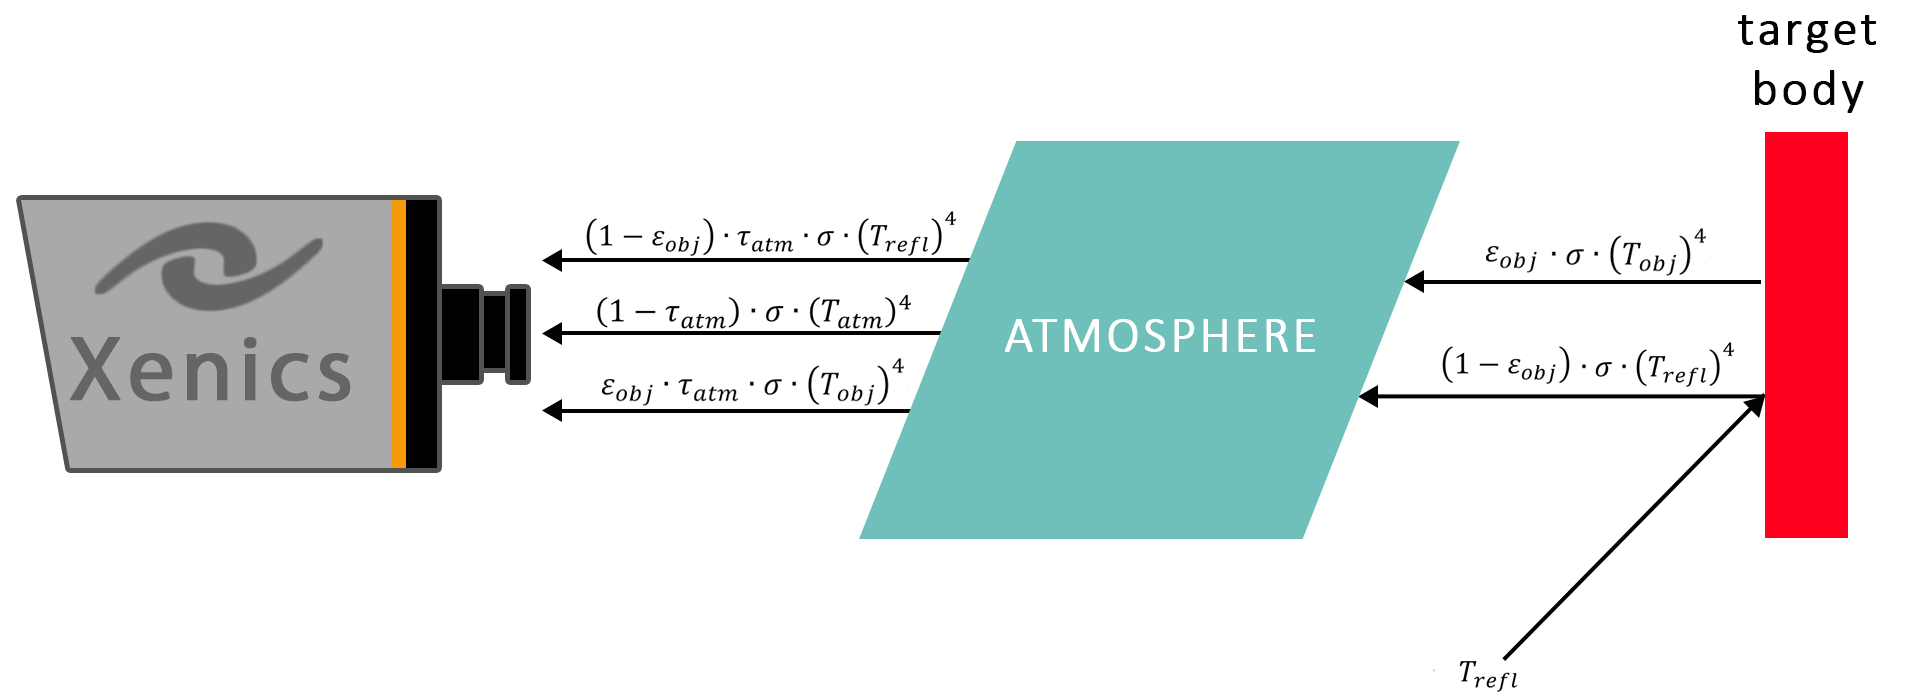
\includegraphics[width=1\linewidth]{Figures/2.Chapter/ir_camera_radiation_scheme.png}
\caption{Total radiation sources scheme}
\label{fig:camscheme}
\end{figure}

\par With these equations it is possible to relate the radiated energy received $W$ and the body temperature. This relation is demonstrated in equation \ref{eq:6} and \ref{eq:7}.
\begin{equation}\label{eq:6}
W_{tot}=W_{obj}+W_{refl}+W_{atm}=(\varepsilon_{obj} \ \sigma \ T_{obj}^4)+((1-\varepsilon_{obj}) \ \sigma \ T_{refl}^4)+((1-\tau_{atm}) \ \sigma \ T_{atm}^4)
\end{equation}
\begin{equation}\label{eq:7}
T_{obj}=\sqrt[4]{\frac{W_{tot}-(1-\varepsilon_{obj}) \ \sigma \ T_{refl}^4-(1-\tau_{atm}) \ \sigma \ T_{atm}^4}{\sigma \ \varepsilon_{obj}}}
\end{equation}
\par The camera receives the total radiation $W_{tot}$, and the user has to input the emissivity and both the ambient and reflection temperatures in the camera software.

\section{Wettability}

\par Wettability is a qualitative surface property that describes how the surface is wetted by a liquid. This property is characterized by the interface tensions between the present solid, liquid and gaseous states. The balance between these tensions is represented in Figure \ref{fig:tensao}
\begin{figure}[h]
\centering
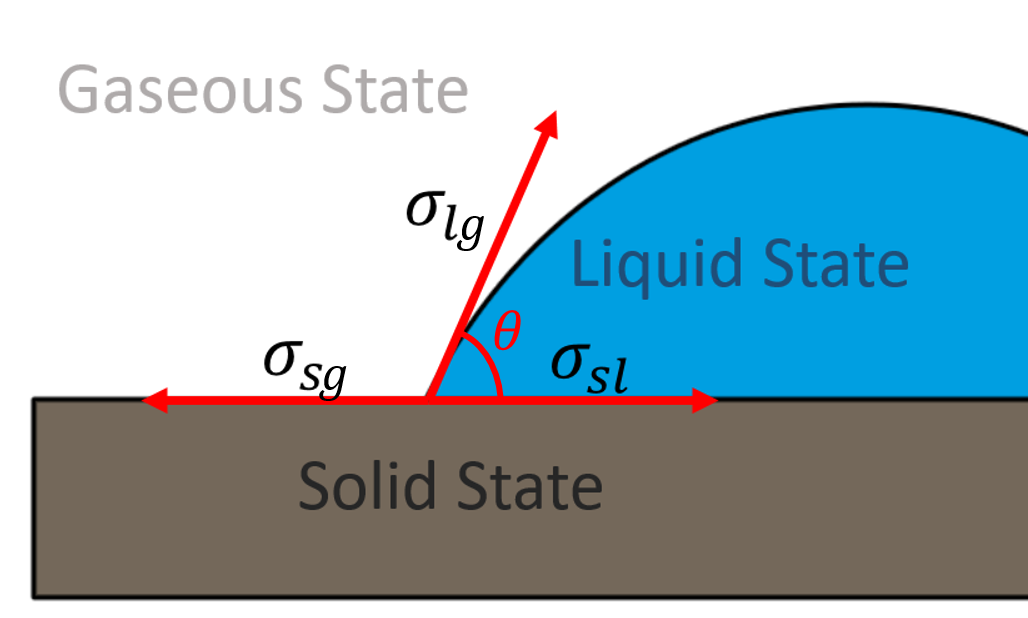
\includegraphics[width=0.5\linewidth]{Figures/2.Chapter/tensao.PNG}
\caption{Tension Balance}
\label{fig:tensao}
\end{figure}
\par Wettability has several parameters that characterize it, being the most used one the contact angle of a sessile droplet onto a flat rigid face. In a thermodynamics perspective, the equilibrium condition of a liquid droplet are calculated by the minimization of the Gibbs energy of the system, G. When one considers constant temperature and pressure conditions it is possible to write the famous Young's equation \cite{young1805essay} from this minimization ($dG=0$), which is simply the tension balance in the horizontal axis:
\begin{equation}
\sigma_{sg}=\sigma_{sl}+\sigma_{lg}cos(\theta_e)
\end{equation}
where $\sigma$ represents the interface tension at the solid-liquid (sl), solid-gaseous (sg) and liquid-gaseous (lg) boundaries and $\theta_e$ represents the equilibrium contact angle. The contact angle is used often to characterize the wettability state of a system. High wettability is considered to have $0\si{\degree} <\theta_e<90\si{\degree} $ and low wettability $90\si{\degree}<\theta_e<180\si{\degree} $. The perfect wetted system has $\theta=0\si{\degree} $ and the perfect non-wetted system has $\theta=180\si{\degree} $ \cite{choi2011wettability}. The Hydrophilic, Hydrophobic and Super-Hydrophobic regimes are defined also by the contact angle and are represented in Figure \ref{fig:wet}.

\begin{figure}[h]
\centering
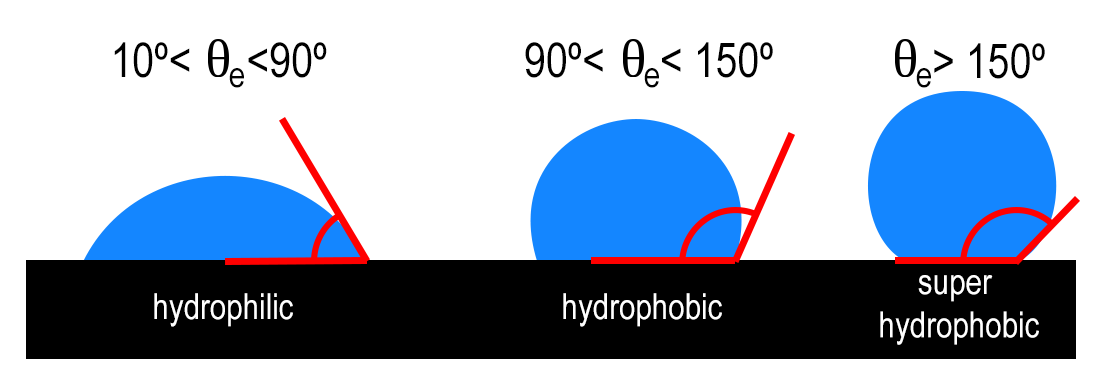
\includegraphics[width=0.7\linewidth]{Figures/2.Chapter/wet.png}
\caption{Wetting Regimes}
\label{fig:wet}
\end{figure}

\par Although it's been assumed that the surface is smooth, in reality one has to take in account the roughness of the surface. Considering an rough homogeneous interface, one can convert the smooth surface contact angle ($\theta_e$) to the actual contact angle ($\theta$) using a formula based on the force balance and empirical correlations, presented in Equation \ref{eq:wenzel}. 
\begin{equation}\label{eq:wenzel}
cos \theta = R_f cos \theta_e
\end{equation}
where $R_f= \frac{A_{SL}}{A_{F}}$ and is the relation between the surface area, to its flat projected area. This equation is called the Wenzel equation \cite{wenzel1936resistance}. Cassie took a different approach and considered an heterogeneous interface, where air would be trapped between the liquid and the surface, in the pockets formed by the surface roughness. So having an interface with a fraction $f_1$ at one contact angle $\theta_1$ and another at $f_2$ and $\theta_2$, the contact angle would be given by Cassie's Equation \cite{cassie1944wettability} :
\begin{equation}\label{eq:cassie}
cos \theta = f_1 cos \theta_1 + f_2 cos \theta_2
\end{equation}
\par The difference between both approaches can be seen in Figure \ref{fig:wenzelcassie}

\begin{figure}[h]
\centering
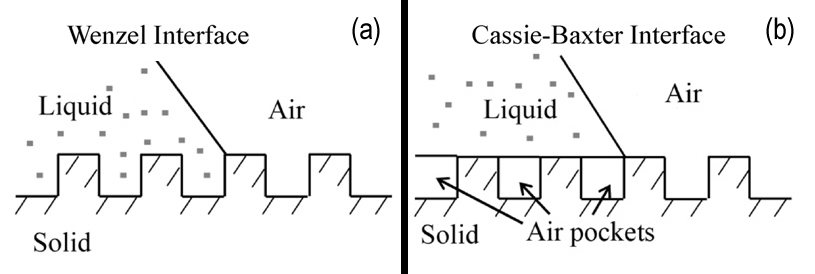
\includegraphics[width=0.7\linewidth]{Figures/2.Chapter/wenzelcassie.png}
\caption{Contact Angle approaches: (a) Wenzel, (b) Cassie-Baxter}
\source{Adapted from Bhushan, 2011\cite{bhushan2011natural}}
\label{fig:wenzelcassie}
\end{figure}


\section{Droplet Impact}

\par During droplet impacts it's possible to categorize the outcome in several categories :

\begin{itemize}
\item Rebound: after the impact the droplet leaves the surface partially or fully. Partial rebound happens when the surface is hydrophobic, and full rebound when it's super-hydrophobic.
\item Stick and Spread: the droplet sticks to the surface after the impact, spreading to its sides. This is characteristic of hydrophilic surfaces.
\item Splashing: the droplet sticks to the surface but smaller droplets are released in the spreading phase. This is influenced mainly by the impact speed and surface roughness.
\end{itemize}

\par When the droplet collides independently of the out come it deforms and spreads. The speed of the \textit{spreading} is dictated by the velocity of the contact edge ($u_{ce}$). This parameter relates with the droplet impact speed ($u_i$) and the contact angle ($\theta$) using Equation \ref{eq:droplet}.
\begin{equation} \label{eq:droplet}
u_{ce}=\frac{u_i}{tan \theta}
\end{equation}

\par During the impact another important parameter to analyze is the spreading factor $\beta$, described in Equation \ref{eq:beta}.
\begin{equation}\label{eq:beta}
\beta=D/d_0
\end{equation}

\par Finally it is possible to prove that the spreading factor grows with the impact velocity ($u_i$) and spreading time using Equation \ref{eq:rein}, taken from \cite{rein1993phenomena}:

\begin{equation}\label{eq:rein}
\beta(\tau)=1-exp(-c\tau) \text{, \quad where} \quad \tau=\frac{t u_i}{R}
\end{equation}

where c is a non-dimensional parameter that depends on the surface tension and R is the droplet radius at that time. This equation is only valid until it reaches the maximum spreading factor.

\par During the \textit{spreading}, when the diameter reaches its maximum value, the droplet assumes a shape similar to a disk. It is after that the \textit{recoiling} phase comes, decreasing the diameter. In this phase, wettability is very important, because it decides whether the droplet will stabilize or leave the surface. While the time-frame for the \textit{spreading} phase is short, the time-frame for the \textit{recoiling} is longer as the interactions between the droplet and the surface. In the final phase, for the hydrophilic surfaces, the droplet reaches an equilibrium diameter. The mentioned phenomena can be seen in Figure \ref{fig:droplet} and Figure \ref{fig:droplethf}.

\begin{figure}[h]
\centering
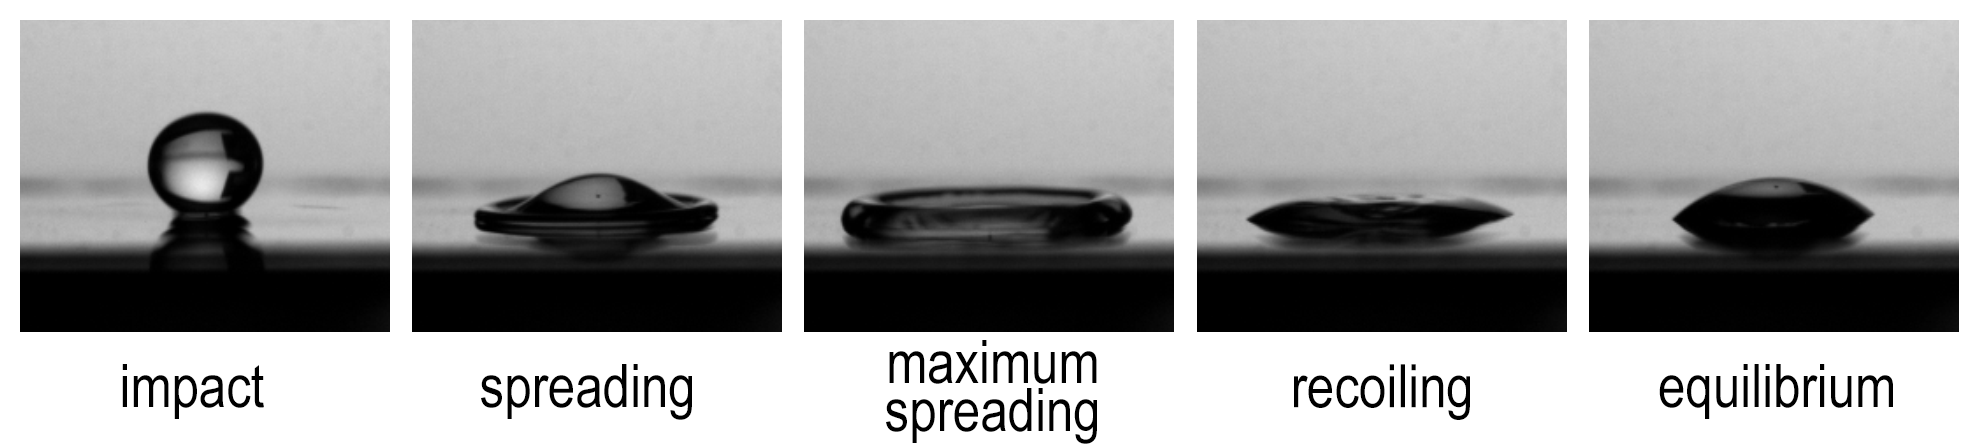
\includegraphics[width=0.9\linewidth]{Figures/2.Chapter/droplet.png}
\caption{Droplet impact stages, for an hydrophilic surface}
\label{fig:droplet}
\end{figure}

\begin{figure}[h]
\centering
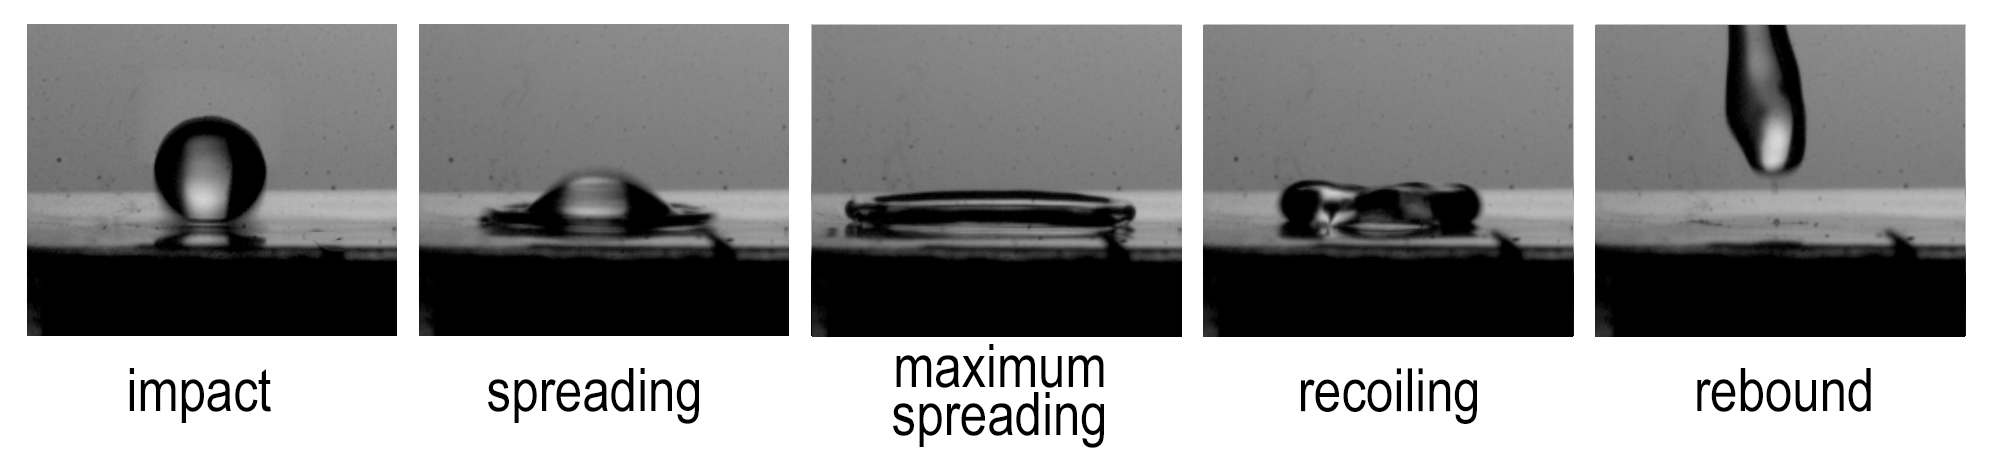
\includegraphics[width=0.9\linewidth]{Figures/2.Chapter/droplethf.png}
\caption{Droplet impact stages, for an hydrophobic surface}
\label{fig:droplethf}
\end{figure}

\par At higher speeds \textit{fingering} may happen. This happens due to instabilities at high Reynolds number that cause the spread droplet to loose its symmetry and form waves at the edge that are called \textit{fingers}. This phenomena can be seen in Figure \ref{fig:fingering}

\begin{figure}[h]
\centering
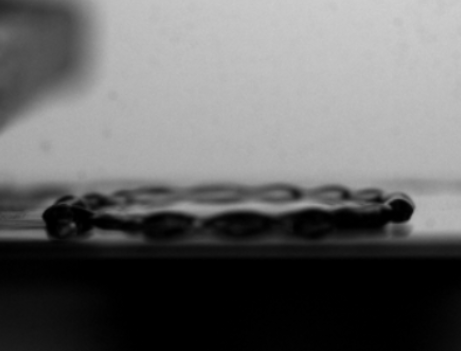
\includegraphics[width=0.35\linewidth]{Figures/2.Chapter/fingering.png}
\caption{Fingering}
\label{fig:fingering}
\end{figure}

\section{Heat Transfer}
\label{sec:heat}

\par During a droplet impact, the most important heat flux to evaluate is the change of heat between the droplet and the heater. According to \cite{sielaff2014experimental}, the heat flux from the droplet can be written as:

\begin{equation}
q''=q_0''+k_h \delta (\frac{{\partial}^2 T}{\partial x^2}+\frac{{\partial}^2 T}{\partial y^2})-\rho_h c_{p,h} \delta \frac{{\partial} T}{\partial t} \quad [W/m^2]
\end{equation}

were $q_0$ is the heat flux from the heater, $k_h$, $\rho_h$ and $c_{p,h}$ are the conductivity, density and specific heat capacity of the heater's material and $\delta$ is the thickness of the heater. Across the radius of the droplet, the heat flux can assume shape shown in Figure \ref{fig:fluxo}. High heat transfer is detected in the first moments before impact, and there is a peak near the edge of the droplet. This is the cause of "new" cold liquid reaching the hot surface. The heat flux is reduced substantially as time passes, mainly because the droplet is heating and the liquid speed is dropping, thus reducing convective and conductive heat transfer.

\begin{figure}[h]
\centering
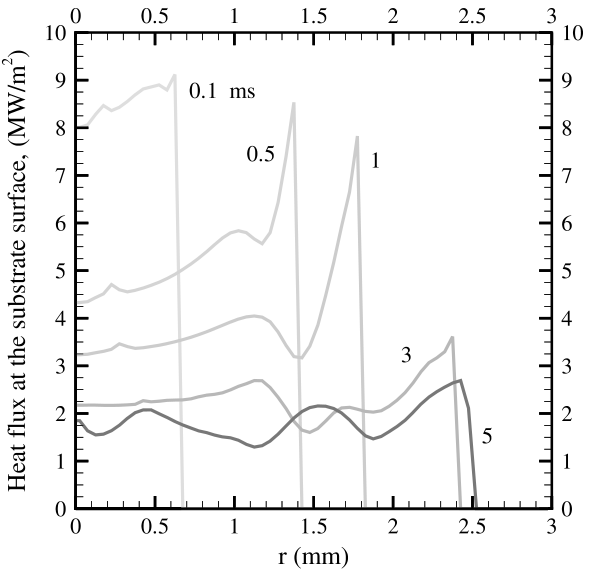
\includegraphics[width=0.5\linewidth]{Figures/2.Chapter/fluxo.png}
\caption {Heat Flux at the surface for different timesteps}
\label{fig:fluxo}
\source{M. Pasandideh-Fard, 2001 \cite{pasandideh2001cooling}}
\end{figure}

\par The power dissipated ($P_{diss}$) by the droplet is the integral of this expression in the droplet area, and it's given by:

\begin{equation}\label{eq:diss}
P_{diss}= \int_{A} q'' \; dA \quad [W]
\end{equation}

\par Because the droplet, ideally, is always axisymetric, it is necessary to decompose $dA$ in cylindrical coordinates. Equation \ref{eq:diss} is expressed in cylindrical coordinates in Equation \ref{eq:cyl}. Integrating the power in time we end up with the total heat extracted. This is expressed in Equation \ref{eq:qtot}.

\begin{equation} \label{eq:cyl}
P_{diss} = \int_\theta \int_r r \, q'' \; dr d\theta \quad [W]
\end{equation}
\begin{equation} \label{eq:qtot}
Q_{tot} = \int_t P_{diss} \; dt [J]
\end{equation}

\par In the work of Pasandideh-Fard \cite{pasandideh2001cooling} is proposed a way to quantify the "cooling effectiveness" ($\epsilon$) of the droplet. This effectiveness is described by the actual heat removed by the droplet divided by the maximum heat transfer possible by theory (assuming no phase change). This coefficient is described by Equation \ref{eq:epsilon}.\\

\begin{equation}\label{eq:epsilon}
\epsilon= \frac{\int_t \int_A q'' \; dA \, dt}{(m c_p \Delta T)_{water}}
\end{equation}

\par The relation between the cooling effectiveness and the time adimensionalized for different impact velocities has already been computed in the past \cite{pasandideh2001cooling} and is shown in Figure \ref{fig:cooling}. The cooling effectiveness grows with the impact velocity because, as shown in Equation \ref{eq:rein}, the spreading factor is larger, meaning that the area covered by the droplet also grows.

\begin{figure}[h]
\centering
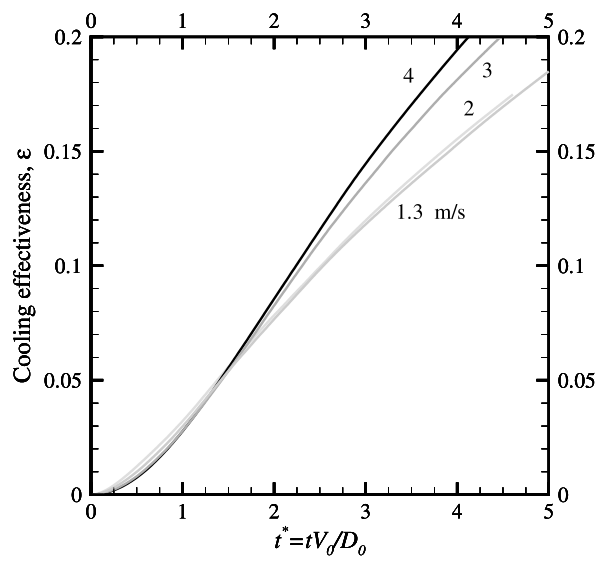
\includegraphics[width=0.5\linewidth]{Figures/2.Chapter/cooling.png}
\caption {Evolution of the calculated cooling effectiveness during the impact of a droplet on a surface initially at 120ºC}
\label{fig:cooling}
\source{M. Pasandideh-Fard, 2001 \cite{pasandideh2001cooling}}
\end{figure}

\par During droplet impact there are many phases that have special heat transfer characteristics. It is described in various sources (e.g. \cite{strotos2011non}) the variation of temperature in the droplet. The Figure \ref{fig:tempvar} illustrates approximately how the temperature of the surface evolves along the radius during spreading. In the center of the droplet the bubble trapping effect creates a barrier for heat transfer, this causes the temperature to have a slightly higher value. Also in the minimum thickness area, also called neck, in the literature, the temperature is higher because the layer of liquid is thinner, removing less heat. In the contact edge, liquid that accumulates there. This liquid comes from the center of the droplet and is colder then the liquid already there, so the temperature decreases again in the edge. The temperature then returns to the heater's temperature, a small distance after the contact edge due to heat conduction in the heater.

\begin{figure}[h]
\centering
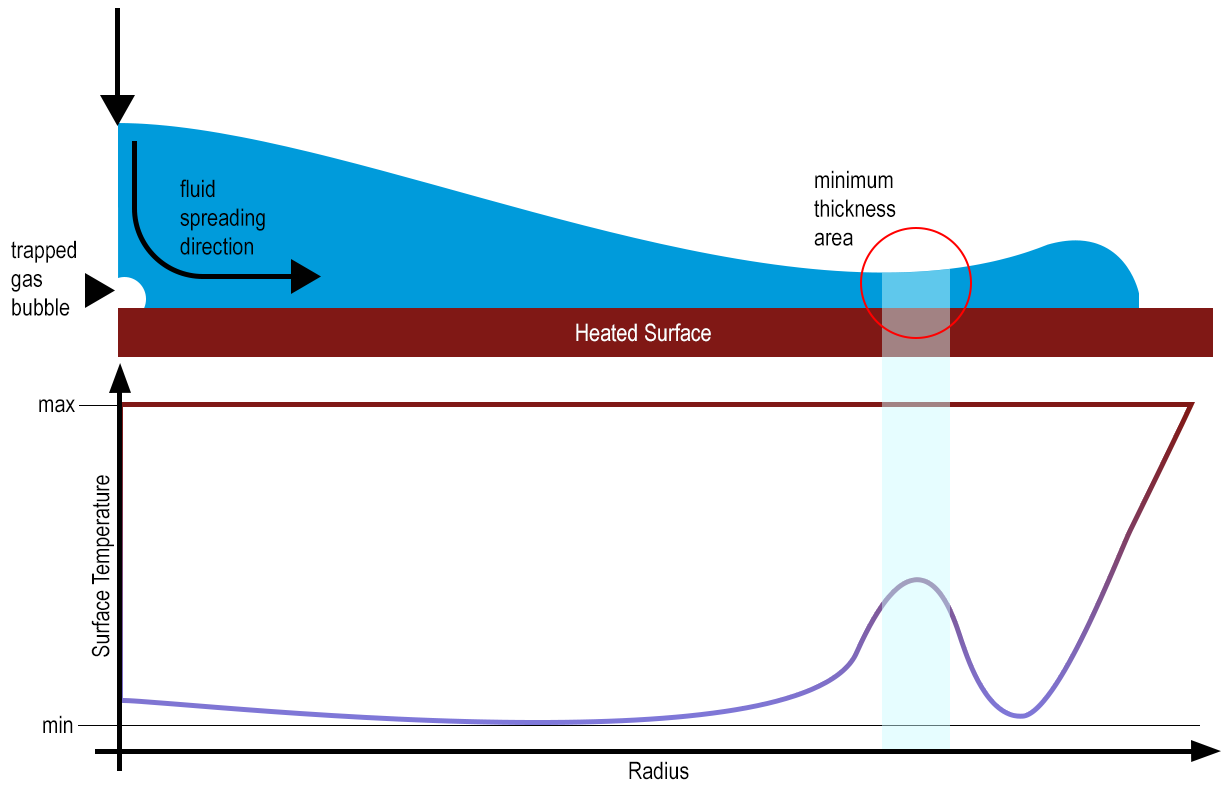
\includegraphics[width=1\linewidth]{Figures/2.Chapter/tempvar.png}
\caption {Scheme of the surface temperature variation along the droplet radius, during spreading}
\label{fig:tempvar}
\end{figure}



\cleardoublepage

\chapter{Experimental Setups}
\label{cap:setup}

\textit{In this chapter the experimental setups used will be shown and explained in detail.}

\section{Introduction}

The experimental setups used in this work had two main themes: droplets on heated surfaces and pool boiling. In the Droplets Experiments a vertical and horizontal view were considered, but in the boiling experiments, because of the water opacity to IR radiation, only the vertical experiment was made.


\section{About the IR Camera}
\label{sec:icam}
The IR Camera, an Onca-MWIR-InSb from Xenics, is the main device used in this dissertation and its function is to give an "image" of the analyzed object's temperature field. Its 2D array of sensors reads the incident IR radiation. Its signal is then converted to temperature in the camera's software. The user will end up with a bi-dimensional field of temperatures with a +/- 0.5ºC precision. This camera can be seen in Figure \ref{fig:onca}.

\begin{figure}[h!]
\centering
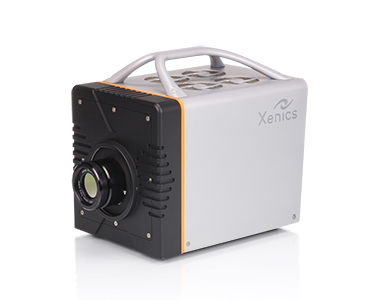
\includegraphics[width=0.6\linewidth]{Figures/2.Chapter/onca.png}
\caption{Xenics' Onca-MWIR-InSb}
\source{http://www.xenics.com/en/onca-mwir-insb}
\label{fig:onca}
\end{figure}

\subsection{Camera properties}

\par The relevant properties of the Onca-MWIR-InSb can be seen in Table \ref{tab:camprop}.

\begin{table}[h]
\centering
\caption{Camera Properties}
\label{tab:camprop}
\begin{tabular}{lclclc}
\toprule
\multicolumn{2}{c}{Camera Characteristics} & \multicolumn{2}{c}{Optical System} & \multicolumn{2}{c}{Image Characteristics} \\
\cmidrule[0.4pt](r{0.125em}){1-2}%
\cmidrule[0.4pt](r{0.125em}){3-4}%
\cmidrule[0.4pt](r{0.125em}){5-6}%
Sensor                 & InSb (MWIR)       & Focal lens          & 13 mm        & Video Rate         & 60Hz                 \\
Spectral Sensibility   & 3.5-5 $\mu m$     & Optics Material     & Germanium    & Max framerate      & 3000 fps             \\
Spatial Resolution     & $320 \times 256$  &  -                  & -            & Min pixels (ROI)   & $15 \times 5$        \\
Thermal Sensibility    & \textless17mk     &   -                 &   -          & Exposition         & \textgreater 1 $\mu s$  \\ \bottomrule
\end{tabular}
\end{table}


\subsection{The Software}

\par This camera has its own specific software, Xeneth, which will be very important throughout this work. It's relevant to explain its functioning, which will be referenced various time in this dissertation.

\subsubsection{Selecting a Calibration Pack}

\par When the program is executed a menu will appear. In this menu it's possible to select not only the used camera (there is also an option to select a virtual camera, used to play previously recorded videos) but also to select a calibration pack as it is shown in Figure \ref{fig:consetup}.
\begin{figure}[h]
\centering
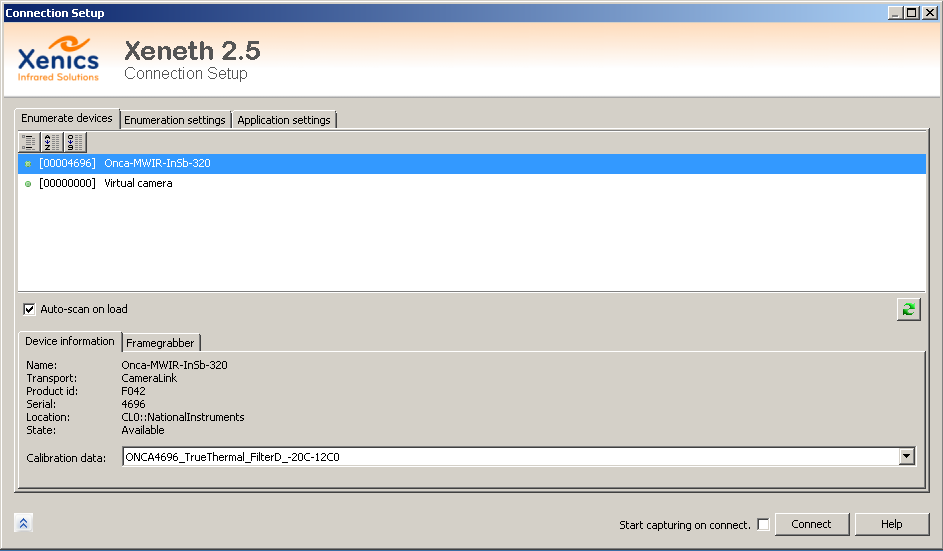
\includegraphics[width=0.7\linewidth]{Figures/3.Chapter/xeneth1.png}
\caption{Xeneth: Connection Setup Menu}
\label{fig:consetup}
\end{figure}
\par In the Calibration data drop menu are available several calibration packs. The main packs are:
\begin{itemize}
\item TRUE NUC: This pack is the one chosen if one wants to get data without temperature conversion. It presents results in ADU (received signal intensity) and it's adaptable to any integration time
\item TRUE THERMAL: This pack comes with a factory made calibration, so the results are presented in Celsius. This is used if the user just pretends a low thermal resolution measure or a qualitative result. It measures temperatures from -20 to 120ºC in any integration time.
\item User Calibration Packs: The user may want to create his own pack adapted to his own temperature interval, to use in a more precise application.
\end{itemize}

\subsubsection{Main Window}
\label{software}
\par After choosing the right calibration for the desired application and before starting the measurements, one should adjust several parameters in the main software window. The displayed panels can be shown in Figure \ref{fig:xeneth2}. There is a panel for the Camera Image, where one can see the thermal image and select an area or dot to take its read value and other statistics; a User Interaction Panel, where one can change settings, view and set the selection properties, record and save videos and choose image filters; a panel that shows the plotted measured data. In the right side we can also see a colour bar. This bar is adjustable so that we can adapt the colour gradient to the desired temperature interval to better observe the phenomena. \\
\begin{figure}[h]
\centering
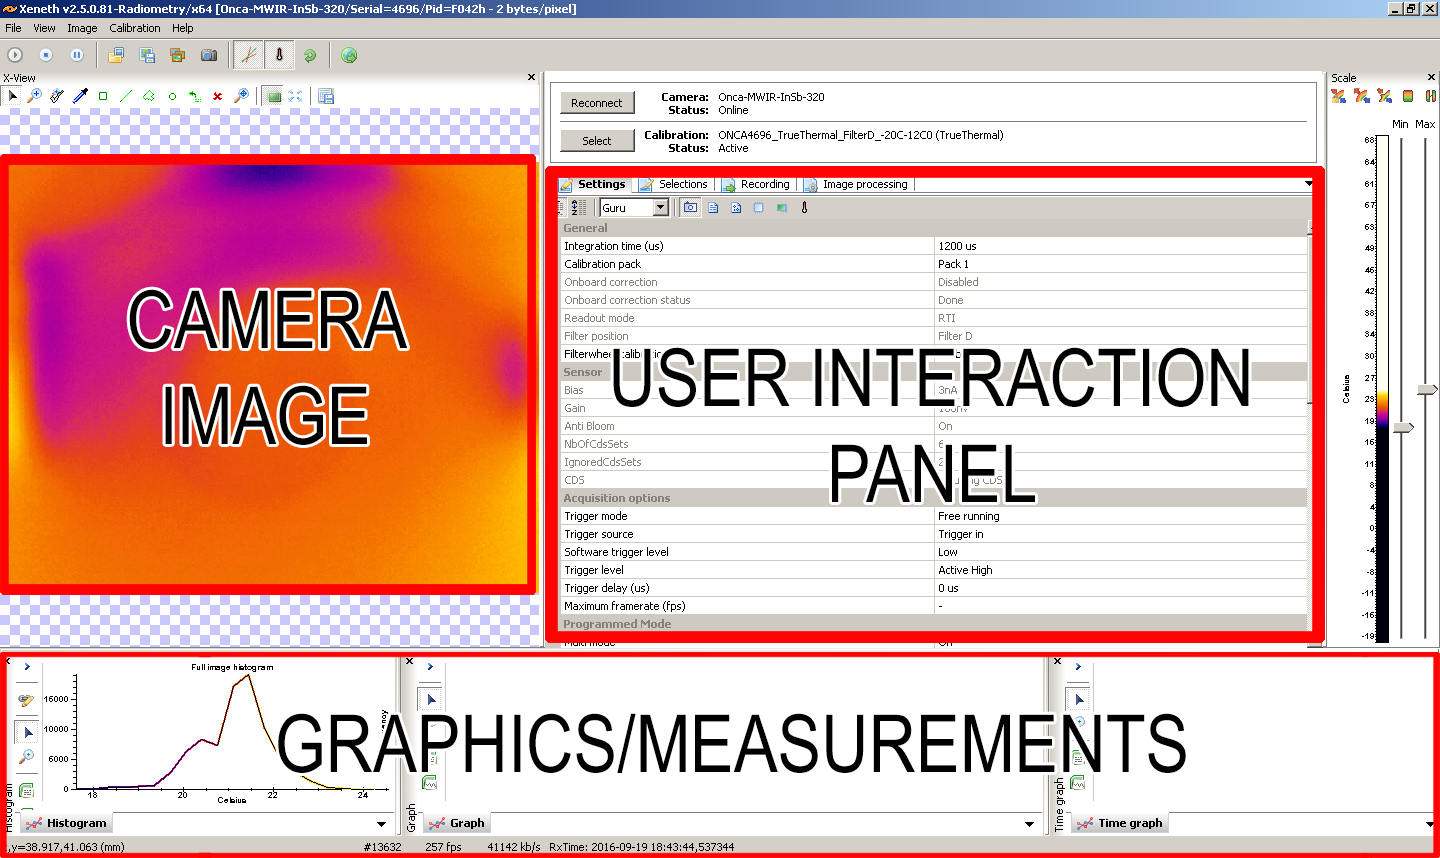
\includegraphics[width=0.7\linewidth]{Figures/3.Chapter/xeneth2.png}
\caption{Xeneth: Main Window Scheme}
\label{fig:xeneth2}
\end{figure}
\par Before starting there are some important settings to review to assure the best image possible. These parameters can be altered in the User Interaction Panel. The first and one of most important parameters is the integration time. The integration time can be easily explained as the equivalent to a common camera's exposure. If we increase the integration time we increase the sensitivity and reduce the noise. On the other side the image will saturate easier, which means that the temperature range highly decreases. So if a higher temperature range is needed, one should decrease the integration time until the desired range is obtained. Increasing the integration time will also affect the frames-per-second (fps) which may not be relevant for static measurements, but the phenomena studied in this dissertation requires high time precision because they happen in the order of milliseconds. The next important value we should consider is the Ambient Temperature and the Atmospheric Temperature. We can also alter this in the User Interaction Panel. To figure out the Ambient Temperature a highly reflective object is put in front of the camera and its temperature measured considering the body to be black. \\
\par The measurements can be made using the Selection Panel, present in Figure \ref{fig:xeneth3}. In this panel it is possible to select a shape (a circle in the case presented) and gather the statistics about the temperature in that area, including average, spatial and temporal deviation. It is also using this method that the temperature of the observed object is measured in this work as it is explain further ahead. Another function in this panel is the Zoom function. It is very important to restrict the measured area as much as it is possible with this function, in order to increase the frames-per-second. \\
\begin{figure}[h]
\centering
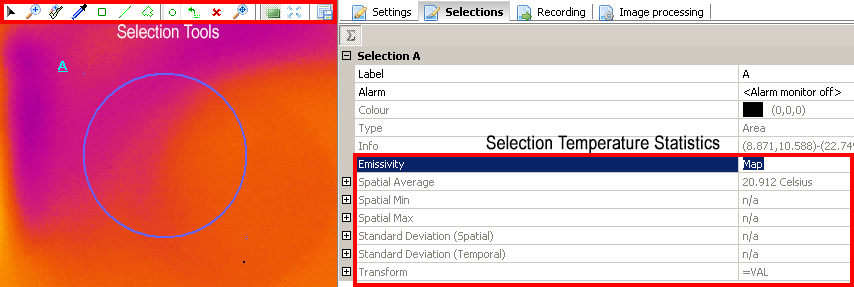
\includegraphics[width=0.7\linewidth]{Figures/3.Chapter/xeneth3.png}
\caption{Xeneth: Selection Panel}
\label{fig:xeneth3}
\end{figure}
\subsubsection{Offset Calibration}
\par When the user selects any of the factory calibrations, there is something that may not seem right. A simple blackbody with constant temperature may appear to have temperature variations as it can be seen in the left of Figure \ref{fig:xeneth5}. This happens due to the Dionisio effect. The Dionisio effect is the reflection of the camera on itself and it is a great error source, so it needs to be eliminated. \\
\begin{figure}[h]
\centering
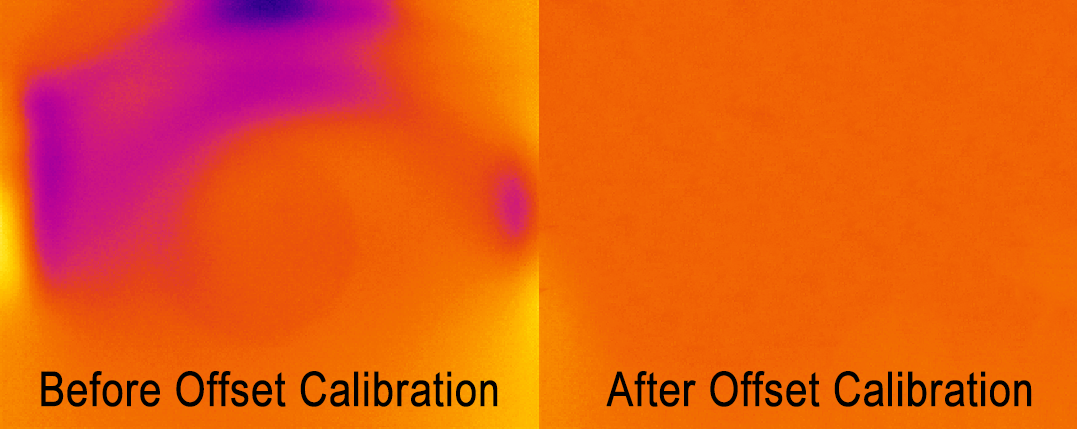
\includegraphics[width=0.7\linewidth]{Figures/3.Chapter/xeneth5.png}
\caption{Offset Calibration: Before and After}
\label{fig:xeneth5}
\end{figure}
\par A good way to eliminate this error is to use a software tool: the Offset Calibration. This can be found in the Calibration Wizard (a menu of calibration options for the camera) and has a simple function. It averages the temperature in space and time and sets every pixel to read that temperature. This eliminates the camera's reflection and also part of the noise and bad pixels. A disadvantage of this method is that it sometimes creates lesser periodic noise, which can be a problem to the measurements. The code behind this function is unknown, so the noise source could not be detected and could only be attenuated later in the post-processing stage. The result of the Offset Calibration can be seen in the right side of Figure \ref{fig:xeneth5}. \\

\section{Droplet Horizontal View}

\par The main objective of this experiment was to observe qualitatively the heat gradients in the droplet as it collides with the heated surface and removes its heat. To create a heater, cartridge resistance heaters were put under an aluminum plate, radiating to its surface. The experiment was made for water droplets, and the surface was hydrophilic. \\

\par To minimize the surface roughness interference a silica wafer was used, thus assuring a droplet fall as symmetric as possible. In the interface of the silica wafer and the aluminum plate a thermal paste was used to improve heat transfer. On top of the silica wafer there is a thermocouple that tracks the surface temperature. This setup can be seen in detail in Figure \ref{fig:horizontal2}. The thermocouple value is used by a PID controller to control the heat released by the cartridge heater. In the PID's screen the temperature of the plate is at its top and the target temperature at the bottom.\\

\begin{figure}[h]
\centering
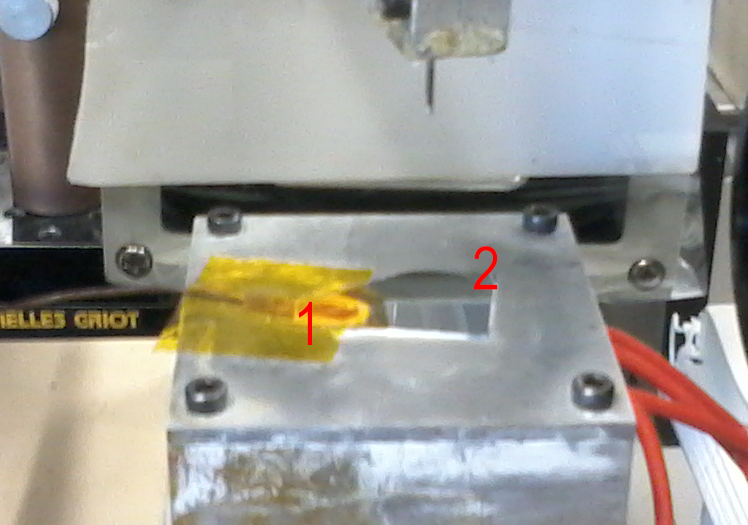
\includegraphics[width=0.5\linewidth]{Figures/3.Chapter/horizontal2.png}
\caption{Silica wafer setup: (1) Thermocouple, (2) Silica Wafer}
\label{fig:horizontal2}
\end{figure}

\par An Harvard Apparatus controls a syringe's water discharge, that then falls from the needle to the wafer. This forms a droplet with 2.6 to 3 mm diameter spherical droplet. This experiment is recorded by 2 cameras: IR camera and high-speed camera. In order for the high-speed camera to work, a high intensity lamp is also needed. The described setting can be seen in Figure \ref{fig:horizontal}. This setting was used to gather qualitative results only. Good quantitative results are impossible due to the implications of droplet geometry in thermography.

\begin{figure}[h]
\centering
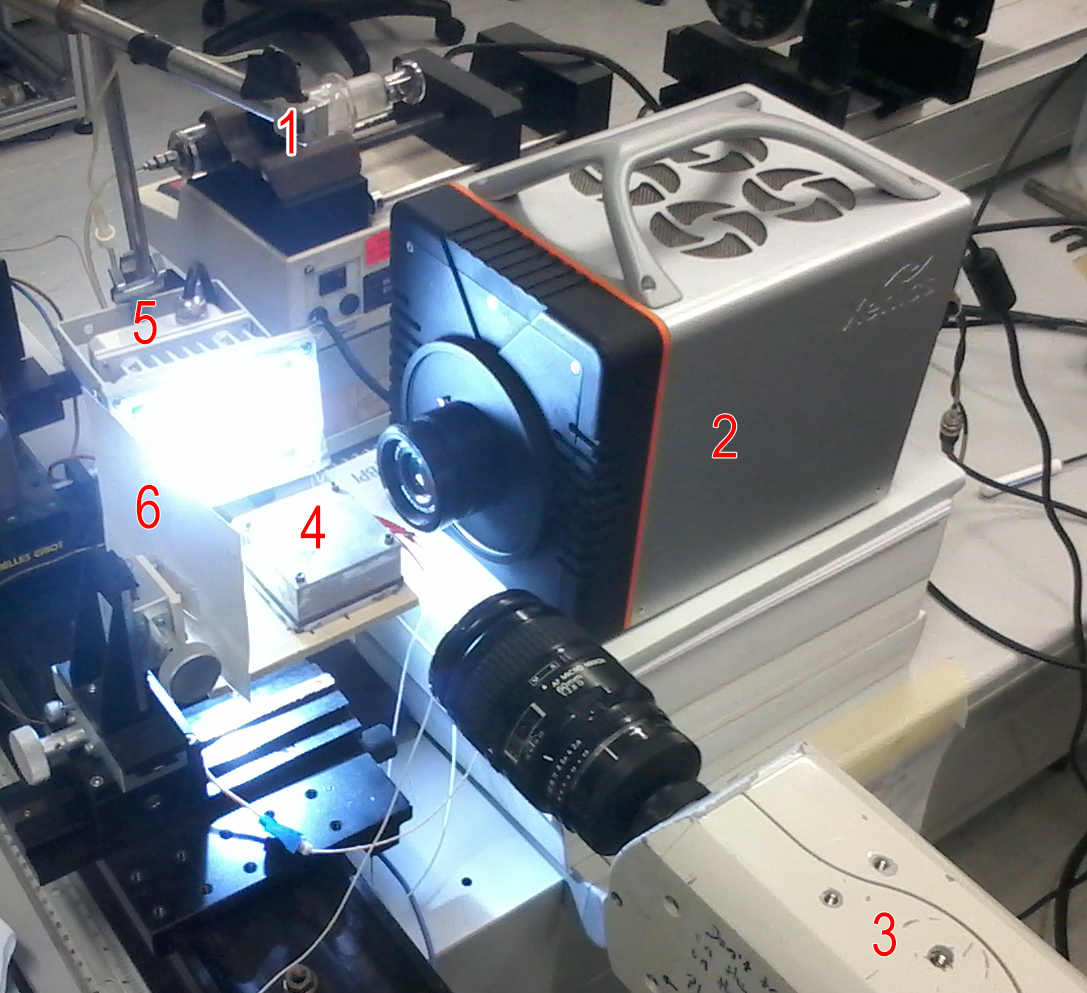
\includegraphics[width=0.65\linewidth]{Figures/3.Chapter/horizontal.png}
\caption{Horizontal setup: (1) Needle, (2) IR Camera, (3) HS Camera, (4) Heated Surface, (5) Lamp, (6) Black Background}
\label{fig:horizontal}
\end{figure}

\subsection{Procedure}
\label{sec:procedure}
\begin{itemize}
\item Adjust IR Camera's settings on the software.
\item Perform an offset calibration (described in Section \ref{sec:icam}).
\item Adjust PID controller to the desired temperature and water flow in the Harvard Apparatus.
\item Turn on the light and set the cameras recording.
\item Let a droplet drop on the wafer.
\item Clean the wafer with acetone and distilled water before proceeding.
\end{itemize}

\section{Droplet Bottom View}

\par The objective of this setup is to observe interface temperatures in during the droplet impact phases. To do this, the IR Camera had to be placed underneath the surface in which the droplet impacts. The droplet impacts on a 20 $\mu m$ thick stainless steel foil. This was done similarly to \cite{sielaff2014experimental}, as the objective was to read the interface temperatures. Because of the small thickness of the foil, the temperature of the interface is very similar to the read temperature in the bottom of the foil. The HS camera was placed horizontally to the foil to observe the impact. A lamp was placed in the opposite site. The setup scheme can be seen in Figure \ref{fig:setup}.\\

\begin{figure}[h]
\centering
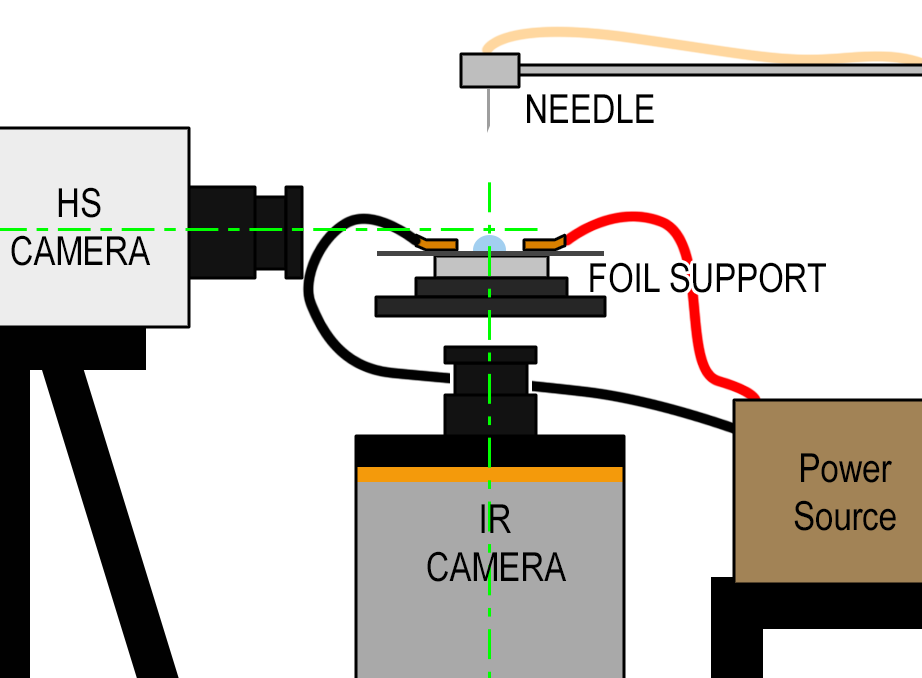
\includegraphics[width=0.55\linewidth]{Figures/3.Chapter/setup.png}
\caption{Bottom Setup Scheme}
\label{fig:setup}
\end{figure}

\par The experiments made around this setup were made using hydrophilic (using distilled water and ethanol) and super-hydrophobic (using just water) surfaces. A preliminary experiment with water and an hydrophilic surface was made, using the software calibration. From the first, raw results were taken for posterior calibration and processing. The calibrations and their differences are explained in Chapter \ref{cap:setup}.\\

\par The foil is fed an electric current, so it can heat up to the desired temperature. This is done by to electrical contacts, wired to a power source. The foil has to be placed on top of a bad heat conductor to minimize heat losses. A heat glass was chosen for the purpose. It also needs to be stretched so that possible wrinkles don't affect the droplet. A detail of the setup, on the foil support can be seen in Figure \ref{fig:suporte}. In this figure two supports are shown. The second was made after the calibration. \\

\par For the case of the super-hydrophobic surfaces, the surfaces needed to be cleaned with an ultra-sound bath and coated with \textit{Glaco}. This coating took several layers to ensure effective coating that can endure high temperature and constant droplet fall. \\

\begin{figure}[h]
\centering
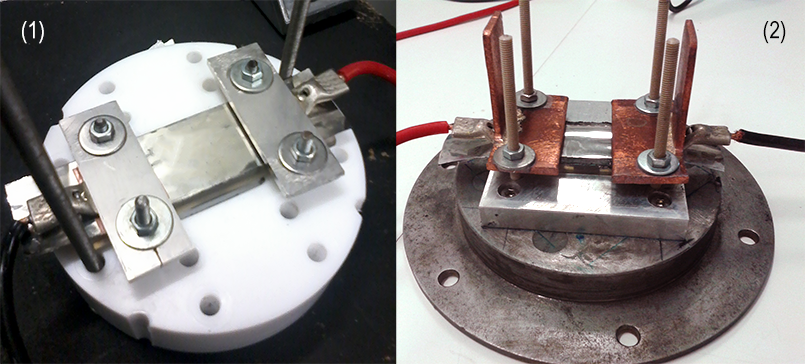
\includegraphics[width=0.9\linewidth]{Figures/3.Chapter/suporte.png}
\caption{Stainless Steel Support: (1) Before calibration setup, (2) After calibration setup}
\label{fig:suporte}
\end{figure}

\par This setup also has the Harvard Apparatus and the needle to create the droplet. A metal structure holds the support, needle and camera. The complete setup can be seen in Figure \ref{fig:setup2}. Although we have a different calibration, the procedure is similar to the previously described in \ref{sec:procedure}. The big difference is that the foil temperature is controlled with the power source and not with the PID. To adjust the current correctly one needs to read the temperature on the IR Camera's software. In the case that raw images are needed, an additional step should be to convert the desired temperatures in ADU. Only this way one can know if the foil is at the desired temperature.

\begin{figure}[h]
\centering
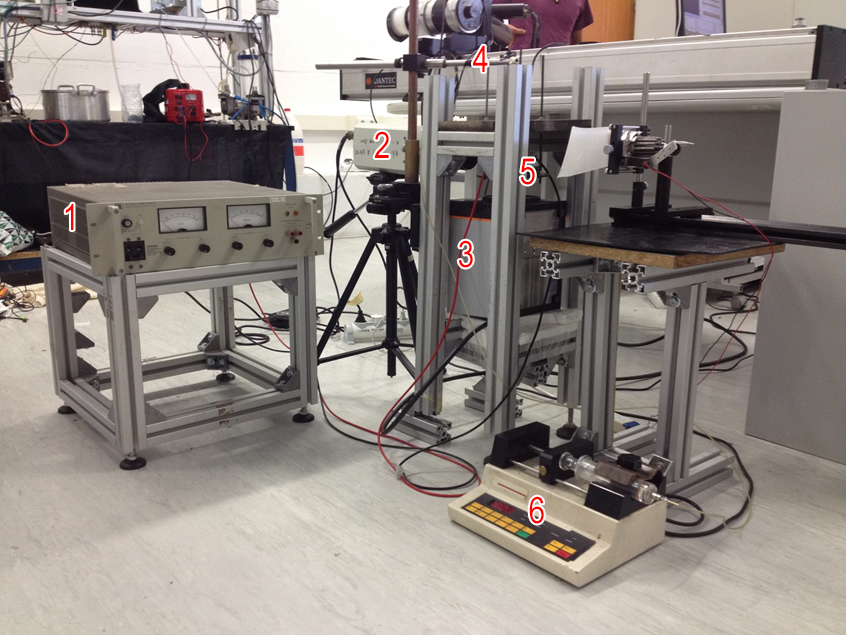
\includegraphics[width=0.9\linewidth]{Figures/3.Chapter/setup2.png}
\caption{Bottom Setup: (1) Power Source, (2) HS Camera, (3) IR Camera, (4) Needle, (5) Foil Support, (6) Harvard Apparatus}
\label{fig:setup2}
\end{figure}
%%\section{Section B}
\label{sec:sectionb}

\subsection{Subsection A}
\label{subsec:subasectionB}

The model described can also be represented as

\begin{equation}
\dot{\mathbf{x}}(t) = \mathbf{T}\mathbf{z}(y),\  \mathbf{y}(0) = \mathbf{y}_0,\  z\geq 0 \\
\label{eq:dummyeq1}
\end{equation}

\noindent where

\begin{equation}
\mathbf{A} = \left[ \begin{array}{cc} -(a_{12} + a_{10}) & a_{21} \\ a_{12} & -(a_{21} + a_{20}) \end{array} \right],\ \mathbf{x} = \left[ \begin{array}{c} x_1 \\ x_2 \end{array} \right] \\
\label{eq:dummyeq2}
\end{equation}


\subsection{Subsection B}
\label{subsec:subbsectionB}

\begin{table}[H]
	\centering
	\caption{Dummy Table.}
	\begin{tabular}{|c|c|c|c|} \hline
		\textbf{Vendor Name} 				& \textbf{Short Name}	& \textbf{Commercial Name}	& \textbf{Manufacturer}	\\ \hline \hline
		\multirow{3}{*}{Text in Multiple Row}		&	ABC				&  ABC\textreg				& ABC SA			         \\ \cline{2-4}
		 								&        DEF				&  DEF\textreg				& DEF SA				\\ \cline{2-4}
										&        GHF			&  GHF\textreg				& GHF SA				\\ \hline
		Text in Single Row					&        IJK				& IJK\textreg				& IJK SA				\\ \hline
		Frescos SA						&        LMN			& LMN\textreg				& LMN SA				\\ \hline
		Carros Lda.						&    \multicolumn{3}{|c|}{Text in Multiple Column}							\\ \hline
	\end{tabular}
	\label{tab:dummytable}
\end{table}
\cleardoublepage
\chapter{Calibration and Data Processing Methods}
\label{cap:setup}

\textit{In this chapter the IR Camera calibration will be discussed. The calibration is a big part of this dissertation, and the work revolving the calibration will be presented here.}
\section{Introduction}
\par The importance of quality calibration for this work is mainly justified by skepticism towards the camera's factory calibration and the quality of the used software. Because the camera's software presents big constraints and brings large sources of mistakes with unknown origins, the best way to process the results is to obtain the RAW data and treat it resorting to a special made Matlab code and a blackbody calibration. \\
\section{Blackbody Calibration Sources}
\par Black Body Calibration sources are recommended by the camera manual to calibrate the camera correctly. They are simply blackbodies with controllable temperature. The temperature controlled blackbody is to be filmed by the IR Camera and the camera's raw data (signal intensity received by the sensors) extracted. With a known temperature and high emissivity it is easy to correlate the signal intensity with the correspondent temperature. Establishing this relation can be done directly in the software but for the reasons referred in the previous section it was done with matlab and excel.\\

\par The Blackbody Calibration Source is the name given to these devices, that are commercialized to calibrate infrared sensors. Because the price of the simplest one can be over 7000 euros, it was decided that one should be created, having in mind the principles of these devices. \\

\par There are several types of blackbody calibration sources, which are included in these main categories \cite{blackbody}: 
\begin{itemize}
\item Fixed-Point Blackbody Radiators: used at really high temperatures (>1000ºC), these are characterized by having a metal (eg. Au, Ag or Cu) at freezing point and a graphite made cavity (high emissivity). The quality of the measure is defined by the quality of the graphite, metal ingot and shape of the cavity.
\item Heat Pipe Cavities: used at temperatures from -60ºC to 1000ºC, depending on the work fluid, these are characterized by having the best precision, and being the most sophisticated devices. They work by having the cavity surrounded by a multistate heated fluid at a controlled pressure. This cavity has special geometric properties to enhance the emissivity of the body. They are usually used in high precision applications like meteorology institutes.
\item Pratical Cavities: used in more pratical applications, their temperature range goes from -45ºC to 450ºC. Unlike the Heat Pipe, the working fluid rarely changes its physical state (eg. one could only go up until 100ºC with water). Pratical cavities have a simpler build and are often used for testing by the radiation thermometers manufacturers. As the latter, Pratical Cavities also rely on specific geometric conditions to enhance the cavity's emissivity.
\item Flat Plate: these devices are used as an alternative to the devices above because they do not require small cavities. With this in mind its obvious the counterpart of this type. The heated plate needs a high emissivity paint and it generates bigger uncertainties. This method is usually used for bigger applications.
\item Others: Cryogenic/Vaccum Blacbodies, used in low temperatures and Furnaces, used as Flat Plate for applications above 1000ºC.
\end{itemize}

\par For this work, the Pratical Cavity Radiator is the best choice, not only because it's often used in the same applications and temperature range but also because it is the simplest solution to produce. The final design of the chamber was based on the scheme presented in Hartmann's work \cite{blackbody}, and it's presented in Figure \ref{fig:bbs} and the cavity shape based on the design proposed in Figure \ref{fig:blkbody}. Because the camera had to be calibrated to work between the temperatures of 0 and 130ºC, the working fluid had to be oil, because of its higher saturation temperature. \\

\begin{figure}
\centering
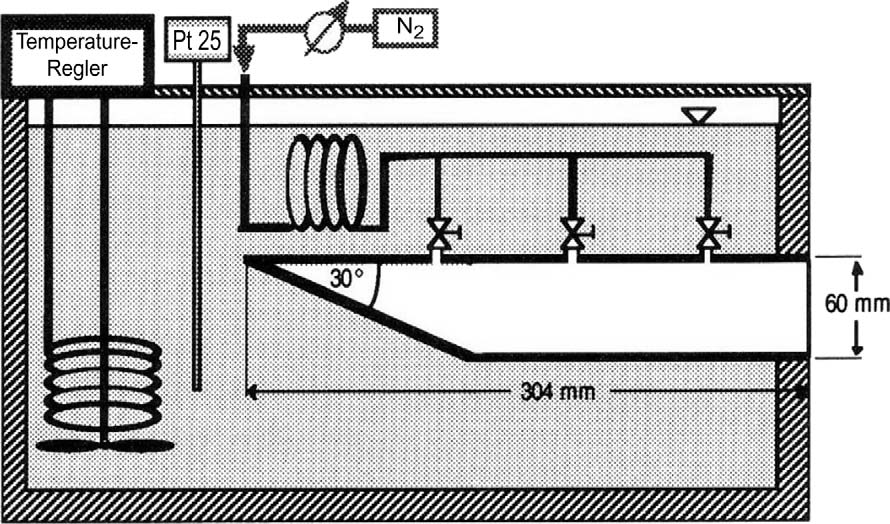
\includegraphics[width=0.6\linewidth]{Figures/4.Chapter/praticalcavity.png}
\caption{Pratical Cavity Blackbody Source scheme}
\source{Chapter 3.2 from \cite{blackbody}}
\label{fig:bbs}
\end{figure}


\par The effect demonstrated in Figure \ref{fig:blkbody} is used in many cavity based Blackbody Radiator Devices and serves to enhance the emissivity, by trapping the light, thus reducing light reflected from the outside. This effect is enhanced by an angle of 30º as referenced in the literature \cite{blackbody}. A working scheme for the final design of the created device, with a mixture of these 2 concepts is presented in Figure \ref{fig:box}. \\

\begin{figure}[h]
\centering
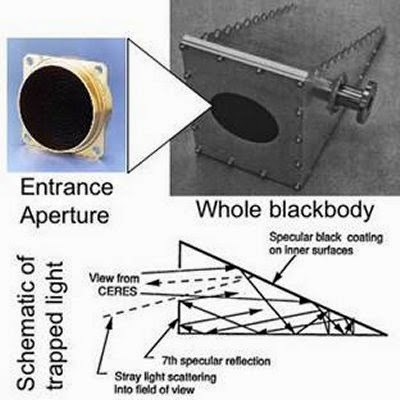
\includegraphics[width=0.6\linewidth]{Figures/4.Chapter/blackbody3.jpg}
\caption{Cavity and light trapping effect scheme}
\source{NASA}
\label{fig:blkbody}
\end{figure}

\begin{figure}[h]
\centering
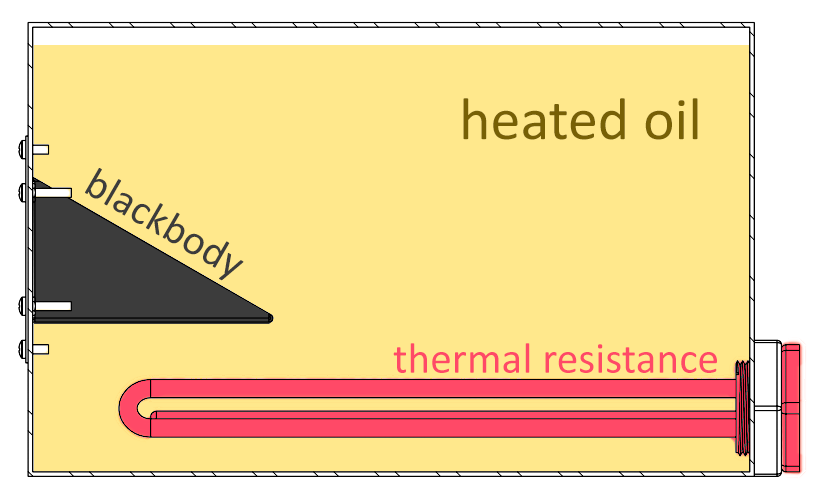
\includegraphics[width=0.6\linewidth]{Figures/4.Chapter/caixa.png}
\caption{Final design scheme for the Blackbody Calibration Source}
\label{fig:box}
\end{figure}

\subsection{Design details}
\par The final design render, made in SolidWorks, can be seen in Figure \ref{fig:render}. One may notice, both from the render and the scheme, that the box is too long compared to the blackbody. The reason for this is that the whole machine had to be made to fit the only available thermal resistance in the store. This resistance is presented in Figure \ref{fig:res}. The working fluid has to be durable and have good conductive properties, so the type of oil used was car oil, due to its durability and thermal properties. \\

\begin{figure}[h]
\centering
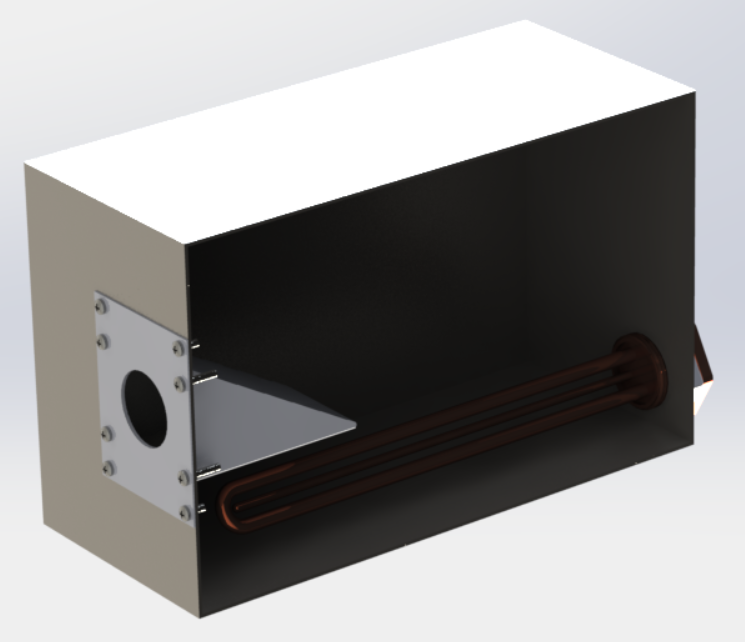
\includegraphics[width=0.8\linewidth]{Figures/4.Chapter/caixa_render.PNG}
\caption{SolidWorks render of a cut device view}
\label{fig:render}
\end{figure}

\par In both the scheme and render, the sensors, peripherals of the machine and its insulation are omitted. In this machine 5 type K thermocouples were used: 2 submerse thermocouples by each side of the blackbody to check if there were high variations of temperature in the oil from one side to another; 3 surface thermocouples to see when the temperature stabilizes in the filmed face, and to have more measurements from which one could take a good average of the real cavity temperature. The scheme for their placement can be seen in Figure \ref{fig:tpar}. \\

\begin{figure}[h]
\centering
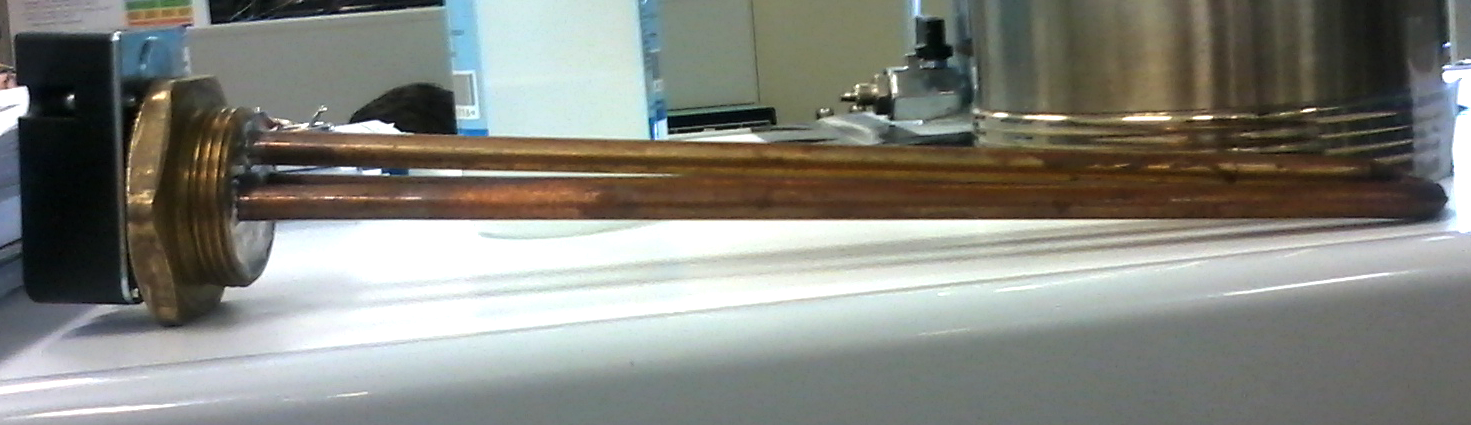
\includegraphics[width=0.9\linewidth]{Figures/4.Chapter/resistencia.png}
\caption{Thermal Resistance used}
\label{fig:res}
\end{figure}

\begin{figure}[h]
\centering
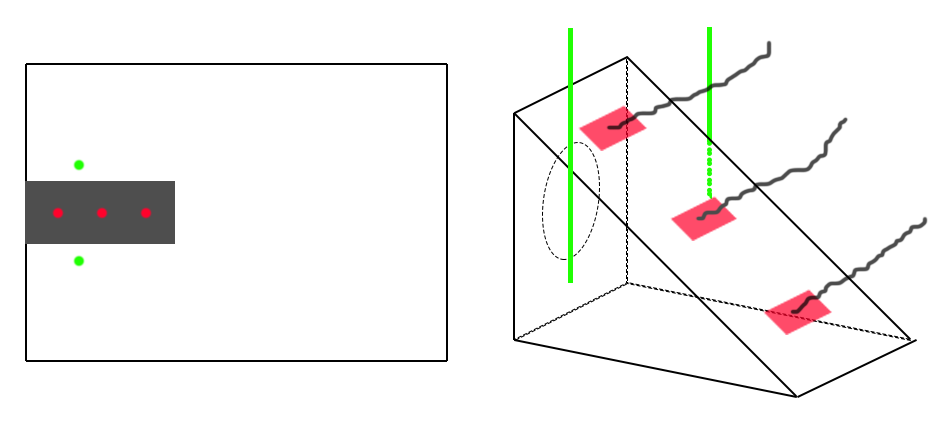
\includegraphics[width=0.9\linewidth]{Figures/4.Chapter/termopares.png}
\caption{Thermocouple placement scheme}
\label{fig:tpar}
\end{figure}

\par The peripherals that the machine needs are: a KS 20-1 PID controller,  that controls the resistance and a DT9828 Data Acquisition Board from Data Translation to connect the thermoucouples to the computer were the data is processed.\\

\par Finally, the insulation consists of a 5mm PENA30FR adhesive, that consists in a sponge with aluminum protection. This can be seen in Figure \ref{fig:isola}. The insulation is used all around the machine and the only hole in it is the hole of the blackbody. \\

\begin{figure}[h]
\centering
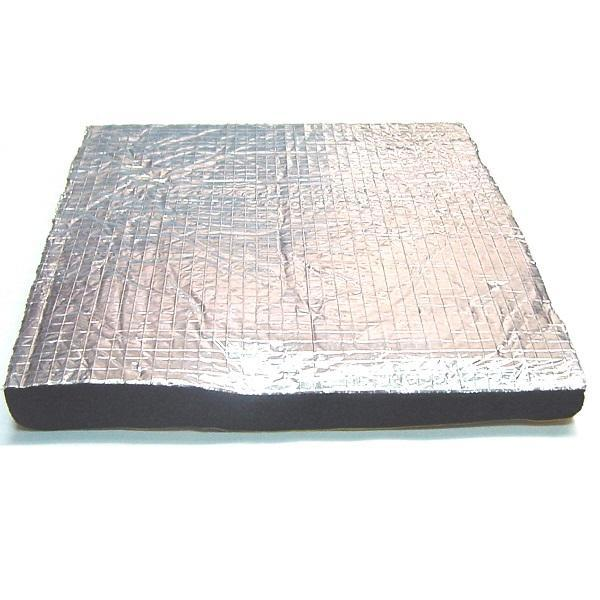
\includegraphics[width=0.5\linewidth]{Figures/4.Chapter/insulation.jpg}
\caption{PENA30FR Adhesive Insulation}
\label{fig:isola}
\end{figure}

\subsection{Building Process}

\par The building process of this machine can be divided in 4 parts:

\begin{itemize}
\item The box: made in stainless steel, this box had to be ordered from a company specialized in metal work. The size of this box is 200x200x320 mm, with 2mm thickness. It already with 2 orifices for both the resistance and the blackbody, but the holes needed to pin the blackbody and sensors to the box had to be made and threaded in the workshop. The thermal insulation was made to fit the box measures. The box is insulated only when both the blackbody and resistance are already installed.
\item The resistance: bought from Mecafil, this resistance was attached to the box with the help of a nut, glued to the back with cold weld. It is also from the resistance hole that all the oil would go in and out. The junction between the nut and the bolt was also reinforced with high temperature silicone, and the screw of the resistance was covered with a Teflon tape to avoid leaks.
\item The blackbody: first a blue print was made and laser cut from a 1mm stainless steel plate, painted with a black matte paint, then bent and finally welded. After the weld, the blackbody had to be re-painted and its insulation reinforced with high temperature silicone. Finally it had to be screwed to its support plate so it could be placed in the box. The end result can be seen in Figure \ref{fig:blkbdy}. This piece was made removable so that new shapes could be made, giving room to the future improvement of the machine. When placed on the machine it is important to put some high temperature silicon to fully prevent any leaks on the machine.
\item The peripherals: starting with the sensors, holes were made on the top of the box so that every sensor could pass through it. The scheme for the holes and the sensors display was already shown in Figure \ref{fig:tpar}. The Data Acquisition Board and the PID controller need to be placed near the box because of the sensor wire length restraint, so a support was made to accommodate everything.
\end{itemize}

\begin{figure}[h]
\centering
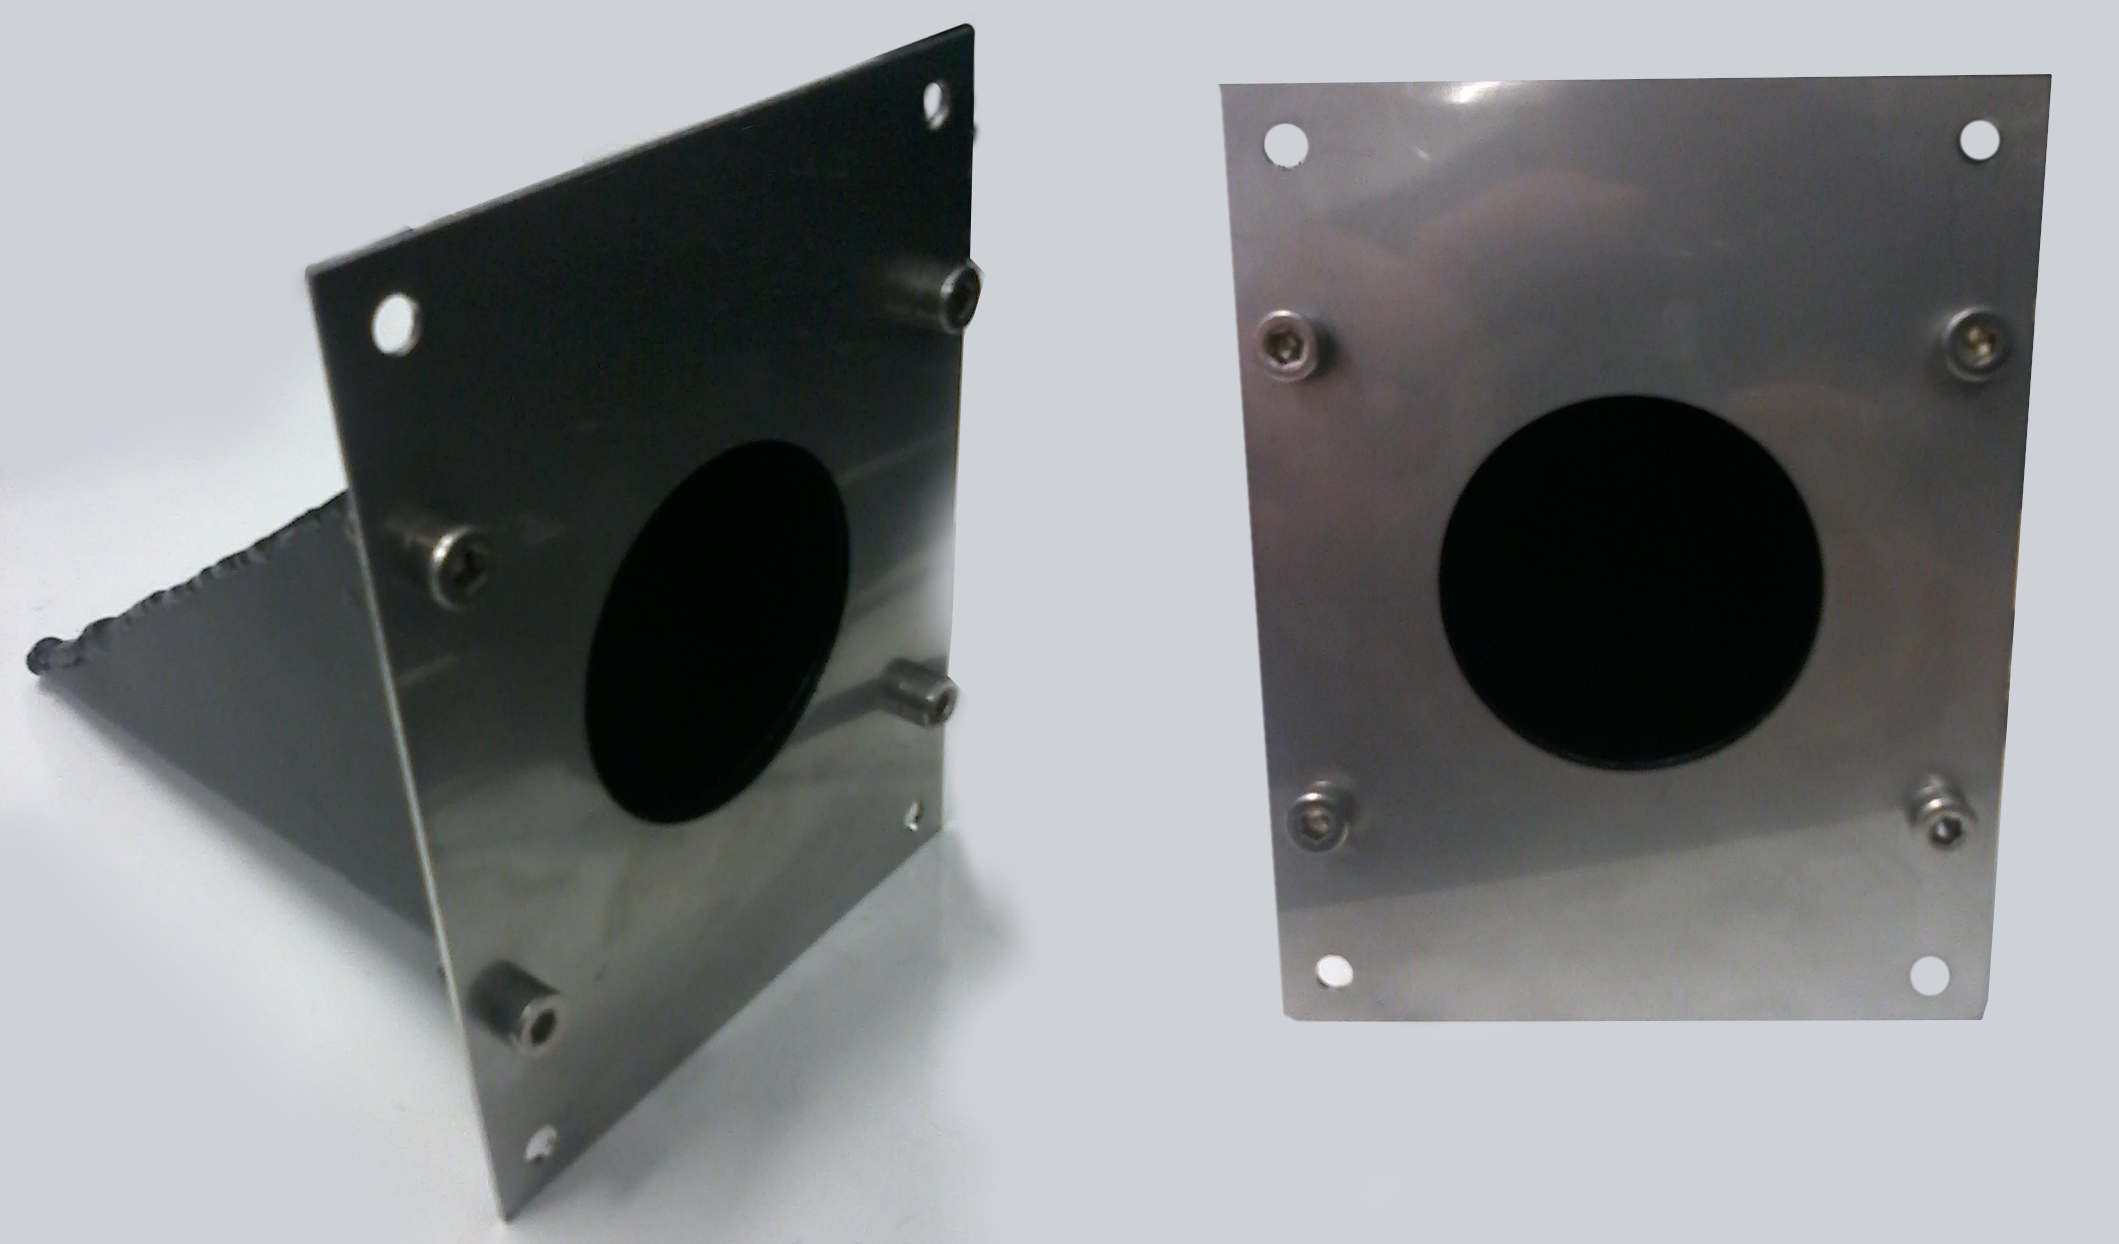
\includegraphics[width=0.7\linewidth]{Figures/4.Chapter/blackbody.png}
\caption{Completed Blackbody}
\label{fig:blkbdy}
\end{figure}

\par The final setup, after all parts were mounted can be seen in Figure \ref{fig:bbcs}. With this setup, it is possible to collect and control temperature values, and correlate them with the camera data, and so it was chosen to perform 2 different calibrations, that will be explained further ahead in this chapter. \\

\begin{figure}[h]
\centering
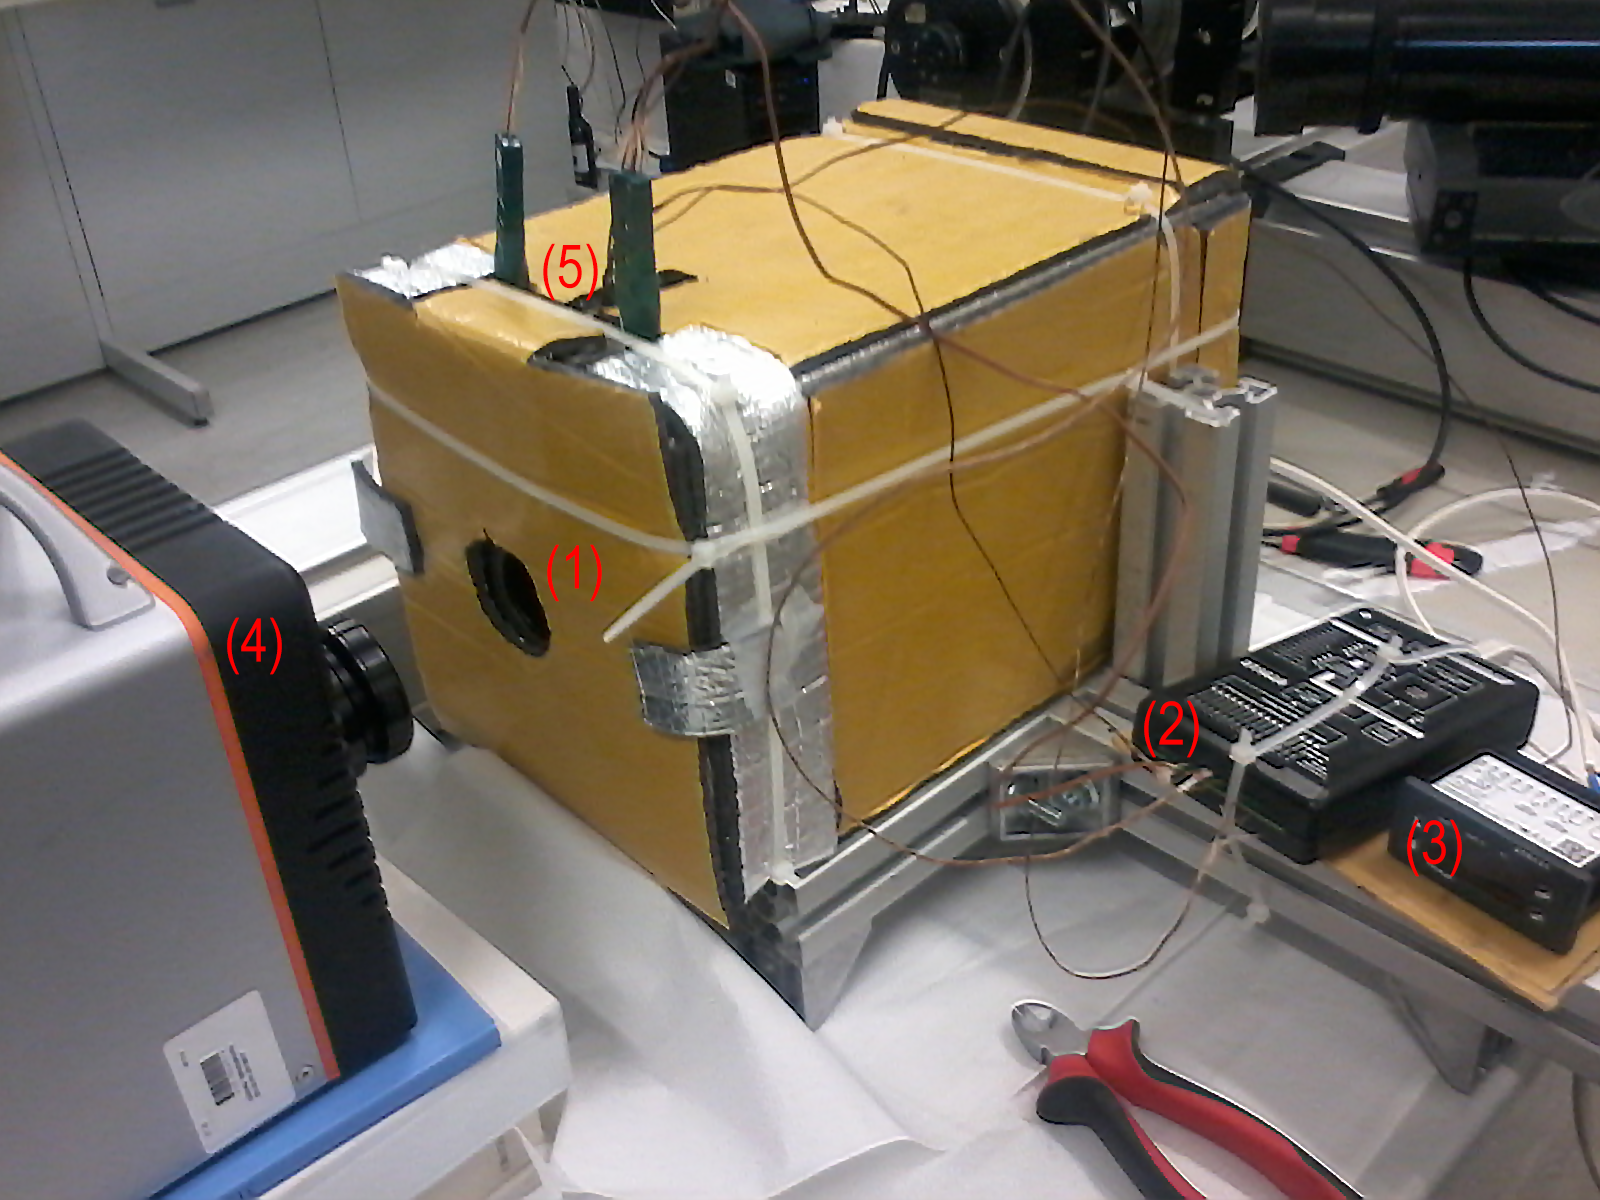
\includegraphics[width=0.7\linewidth]{Figures/4.Chapter/complete.png}
\caption{Completed Blackbody Calibration Source: (1) Blackbody cavity; (2) Data Aquisition Board; (3) PID controller; (4) IR Camera; (5) Thermocouples (one connected to the PID, the others to the Data Aquisition Board)}
\label{fig:bbcs}
\end{figure}

\section{Calibration process}

\par Before the calibration begins there is a set of steps that one needs to take to do it properly:
\begin{itemize}
\item Fill the machine with oil. The oil needs to be taken out of the box after the experiments so it stays clean and it can be stored.
\item Connect the thermocouples to the Data Aquisition Board and to the PID.
\item Turn on the IR Camera and open both its software (Xeneth) and the board software (QuickDAQ).
\item Define an adequate integration time to the desired temperature interval.
\item Do an offset calibration with the camera software.
\end{itemize}

\par It is possible to calibrate the camera in 2 ways now, we can either use the software's calibration feature or use an excel sheet and write the medium ADU value of the cavity region, and then preform the calibration in the post-processing phase. The latter proved to be the best method, but both will be analyzed. \\

\begin{figure}[h]
\centering
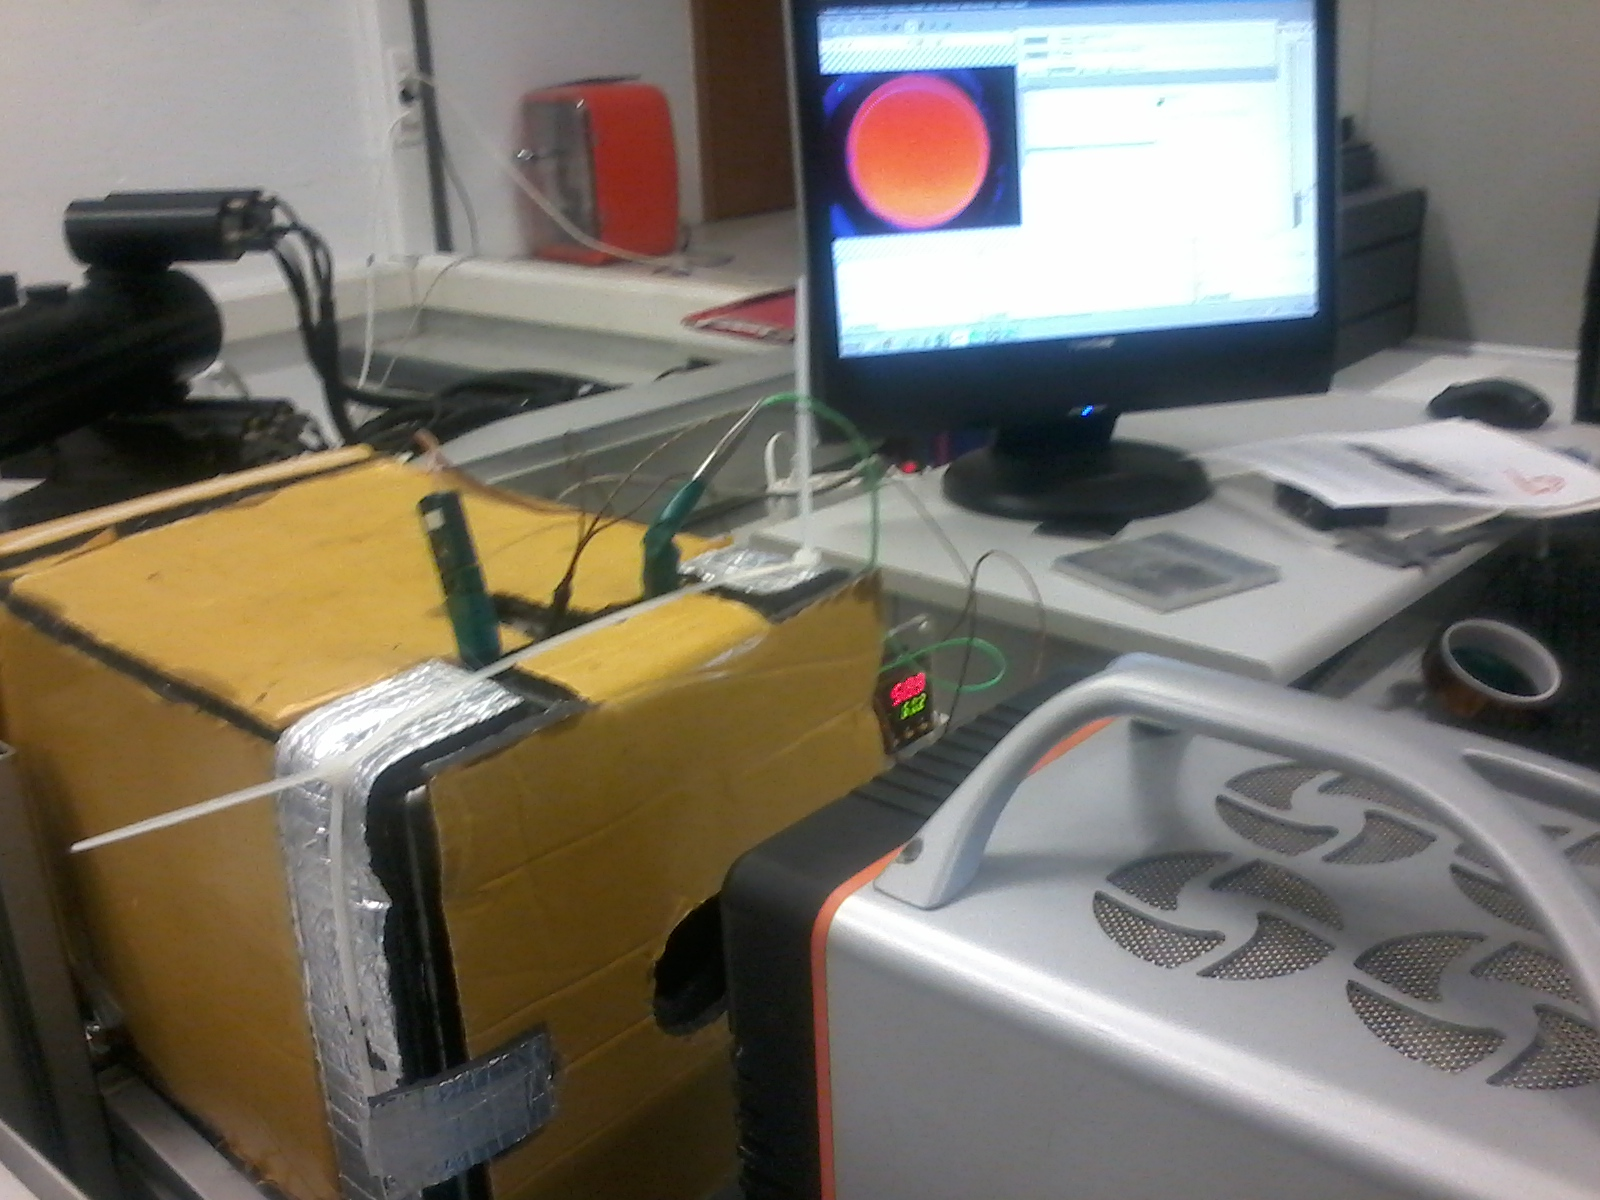
\includegraphics[width=0.55\linewidth]{Figures/4.Chapter/calibinprog.jpg}
\caption{Calibration Instalation in Function}
\label{fig:calibinprog}
\end{figure}

\begin{figure}[h]
\centering
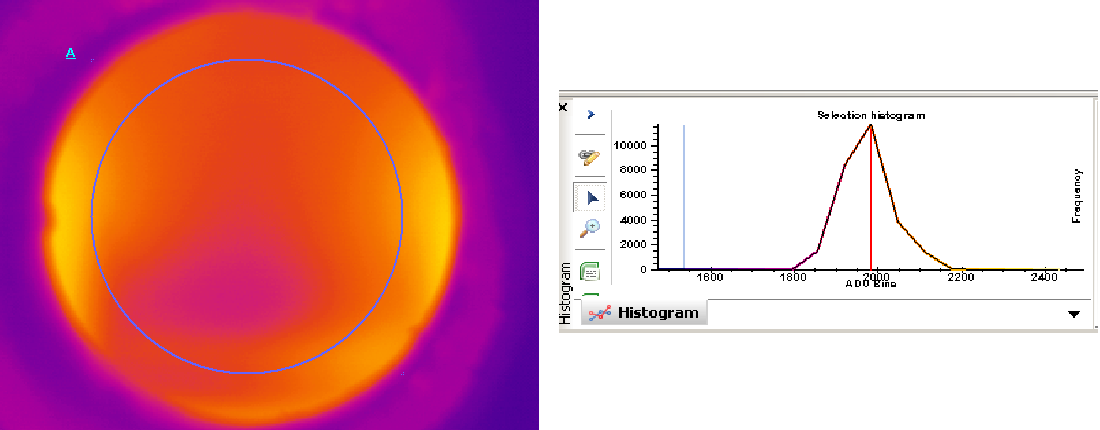
\includegraphics[width=1\linewidth]{Figures/4.Chapter/ex11.png}
\caption{Blackbody thermal image and its respective histogram}
\label{fig:ex1}
\end{figure}

\par During the calibration, the installation looks like Figure \ref{fig:calibinprog}. The first step is to insert the desired temperature (starts with the ambient temperature and then scales in increments of 10ºC/20ºC between measurements) and wait for the temperature to stabilize. In the beginning, what the user will see is shown in Figure \ref{fig:ex1}. It is noticeable here that the edges of the cavity are hotter than the rest. This is due to the fact that the weld that has different thermal properties that the metal sheet, and so it isn't possible to make a calibration right now. \\

\par This may be a problem, but the PID controller solves it. The following is a simplified description of how the PID controller works to give context. A temperature is inserted in the PID controller, then compares it with the thermocouple's temperature and if the thermocouple's temperature is below the desired temperature it turns on the resistance. Just before the oil is at the desired temperature, it turns off the resistance in order to account for the response delay. When the resistance is off the temperature cools and when it reaches a certain temperature bellow the desired temperature, it turns on the resistance again. This cycle is repeated to keep the system at the desired temperature. \\

\begin{figure}[h]
\centering
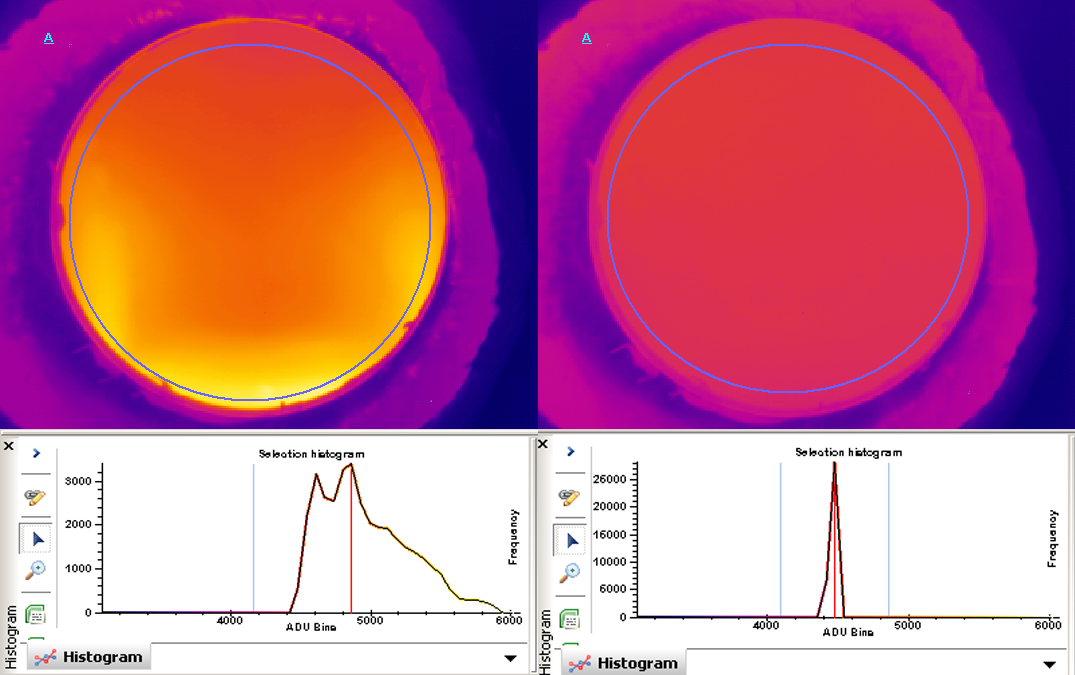
\includegraphics[width=0.9\linewidth]{Figures/4.Chapter/ex2.png}
\caption{Xeneth's software - Temperature Calibration (Plank)}
\label{fig:ex2}
\end{figure}

\par With this context given, it is possible now to explain how can we get an uniform temperature on the cavity. When the resistance is off, because of the thermal inertia of the oil and the good insulation of the machine we can get a more uniform temperature, as it stabilizes while cooling down. This can be clearly seen in Figure \ref{fig:ex2}. In the left we have the temperature map once we reach the desired temperature for the first time. After a few minutes, it is possible to see what's in the right. Please pay attention to the histograms for they show exactly what is desired for the ideal temperature measurement: in the left we can see a wider range of values, and in the right there is clearly a peak. This means that on the circle marked as A the temperature got much more uniform and it's now possible to take a measurement. \\

\par To see what temperature corresponds to the averaged ADU value, an average of the surface thermocouple read temperatures in time was taken, with the help of the software QuickDAQ, which allows to take a data sample for a fixed amount of time. This is used to make the average between all the surface thermocouples connected to the board and the value shown in the PID. This final average is then the input for the software calibration or saved with the ADU in an excel for the second method. \\

\subsection{Software Calibration}

\par The Xenics' software has a camera calibration wizard (in which the offset calibration feature is included) that automatically correlates the ADU's with temperature measured. The feature described is called "Temperature Calibration (Plank)" and can be seen in Figure \ref{fig:plankcalib}. In the shown interface, the user can input the temperature measured by the thermocouples in the field (a), and then add the read value with button (b). It will then add a point, to the table at the left and draw in on a graph bellow. This point has the given temperature, and the ADU measured with a spatial average of a small rectangular area in the center of the image. \\

\begin{figure}[h]
\centering
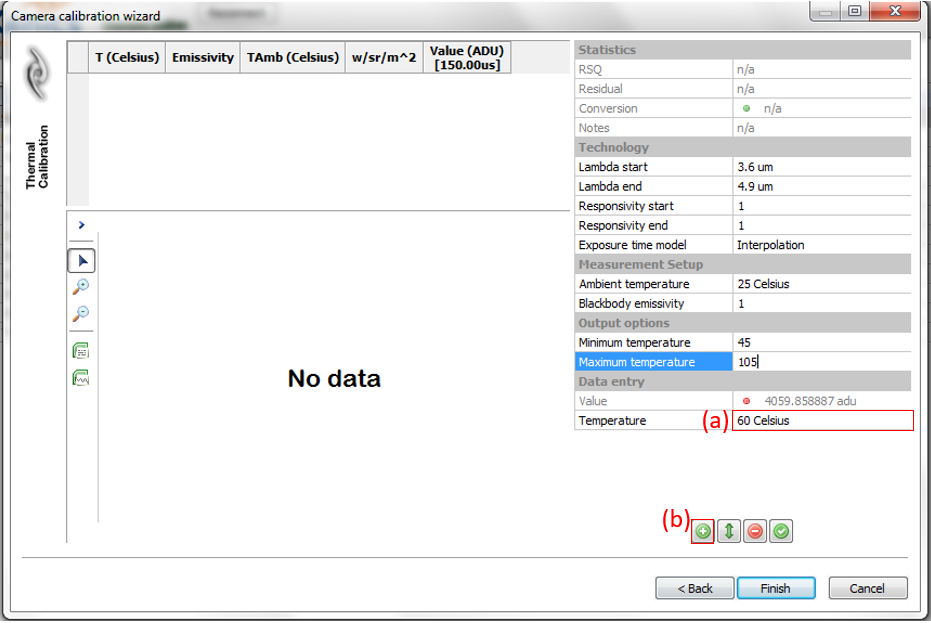
\includegraphics[width=0.7\linewidth]{Figures/4.Chapter/plankcalib.png}
\caption{Xeneth's software - Temperature Calibration (Plank)}
\label{fig:plankcalib}
\end{figure}

\par In the first calibration, this method was tried but because the temperature and respective measured ADU are shown it didn't invalidate the possibility to use them in the second method. In this attempt the integration time of 450 was used. The final table and graphic can be seen in Figure \ref{fig:calib}. On the table labeled as (a) it's possible to see 5 columns. The first column and the last represent the read values of temperature and ADU. The second and third column represent the ambient temperature and emissivity which are actually irrelevant for this case because we are assuming we have a perfect blackbody, so the ambient temperature won't be used in this calibration. The fourth column is a variable, which varies with the input temperature, that the software uses to convert, together with the other inputs, the temperature, in what the software calls "Soaled Radiance", represented in the x axys of graph (b) in Figure \ref{fig:calib}. This variable is not explained in the manual, nor its relation with the temperature. This was one of the disadvantages of this method mainly because the software creates the "Soaled Radiance" value out of it, and it is supposed to mantain a proportional relation with the ADU's so the calibration is described by a line. But as it is noticeable in the graph, the values didn't follow the line that closely, which caused a deviation significant enough to make this method unusable. \\

\par Having this variable and the "Soaled Radiance" unexplained, the only option was to take these values and use them in the other method. Another reason is that this method does a linear correlation. This may only be a vague assumption or a rough approximation, and because even if the origin of these variables was known, there would be no way to validate that linear relation. \\

\par In the end, the software creates a calibration convertion that can be selected when it is opened and used to take the data directly in Celsius. This calibration file can only be used for the specified integration time. In Figure \ref{fig:calib} it's possible to see how the software approximates linearly (green line) the measured points (red line). Because this calibration didn't match the experimental values as close as desired, when the newly created calibration pack was tested it didn't work properly, so the second type of calibration was made. \\

\begin{figure}[h]
\centering
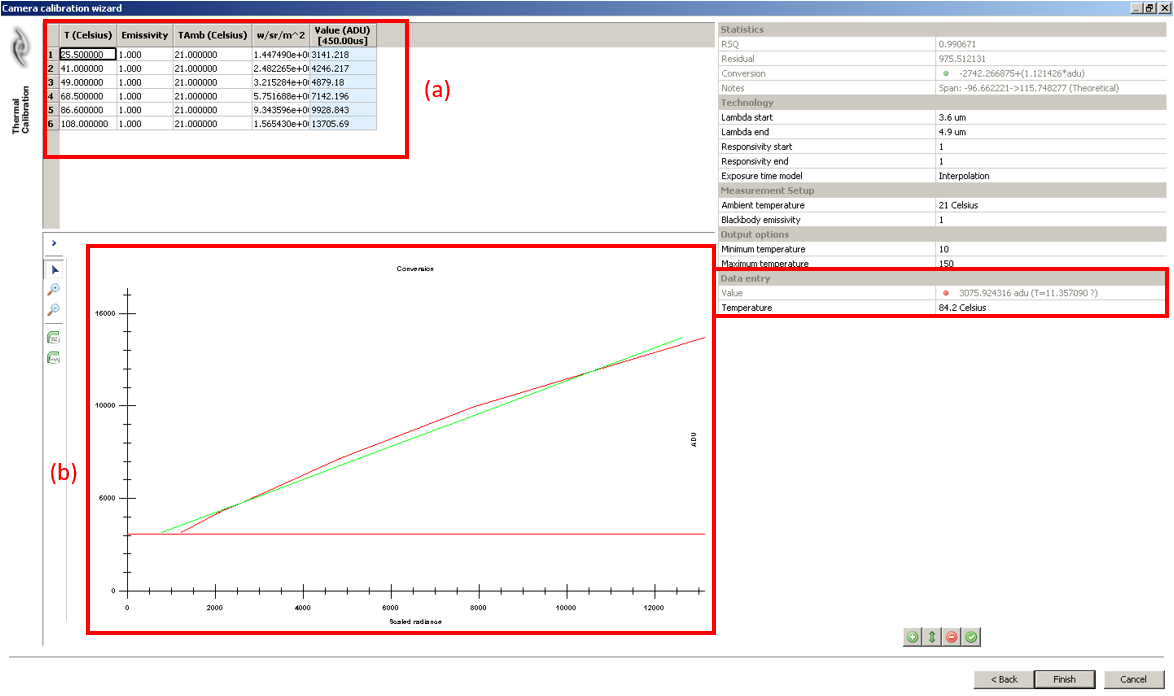
\includegraphics[width=0.7\linewidth]{Figures/4.Chapter/calibracao.png}
\caption{Complete Temperature Calibration (Plank)}
\label{fig:calib}
\end{figure}

\subsection{Proposed Calibration}

\par In this method the calibration results are taken directly from the software, without using the software's Calibration Wizard. They're saved in an Microsoft Excel sheet along with the average temperature read by the thermocouples. With this method the results have to be taken raw from the software and then process them with the matlab code that was made just for this purpose. A whole explanation of the process will be given in the next section, leaving in this section a general outline of the proposed method.\\

\par The process of data aquisition for the calibration is similar to the previous calibration. The main difference in this method is the absence of the Calibration Wizard. Instead, the Selection Panel (described in \ref{software}) is used to gather the average measured ADU of a circular area, similar to what can be seen in Figure \ref{fig:ex2}. There are several advantages in this method, one being that it was now possible to adjust the temperature range (the Calibration Wizard didn't allow it), and better understand when the image saturates. Another advantage is the fact that it is possible to change integration time. \\

\par In Microsoft Excel, the measured temperatures are converted into the radiated energy using equation \ref{eq:6} (and considering the object perfectly black) and plotted against the ADU. Then Microsoft Excel's trending line function is used to extract a polynomial curve that will best approximate the data gathered in the experiments. The second and third degree polynomial approximations were compared, but in the end the third degree polynomial. This option took longer to process but the end result was significantly closer to the experimental results. \\

\par With the extracted curve a MATLAB code was made to calibrate the videos. The raw data video data (in ADU) matrix is the input of this function. This matrix has the value for every pixel in every frame, and point by point is solving the following equation:

\begin{equation}
A \times W_{tot}^3 + B \times W_{tot}^2 + C \times W_{tot} + D = ADU_{pixel}
\end{equation}

in which A,B,C and D are the coefficients of the calculated polynomial curve, $ADU_{pixel}$ is the pixel ADU value and $W_{tot}$ is the wanted radiated energy. Using this radiated energy value, the pixel temperature is calculated using equation \ref{eq:7}. The end result is a matrix with all the temperatures.

\subsection{Calibration Process Details}

\par One important fact about the designed calibration procedure is that it took a whole day to complete. This is due to the fact that there was no refrigeration system and the liquid had to cool at room temperature. It would also have some problems at high temperatures with leaks. This took some time to address and caused that the calibration process couldn't often be repeated. \\

\par Two calibrations were made during this work. The first was made using the software at the fixed integration time of 450us. The second was made using the proposed method for the integration times of 450us and 200us. With the integration time of 450us the image would saturate at around 108ºC, so the correspondent results weren't suited for our experiment. \\

\par The results of the calibration can be seen in Table \ref{tab:calibration}. Because the results were taken for both calibrations at $it=450us$ we can use them to prove the method's consistency. The comparison can be seen in Figure \ref{fig:calibplot}.  \\

\begin{table}[h]
\centering
\caption{Calibration Results}
\label{tab:calibration}
\begin{tabular}{ccccccccc}
\toprule
\multicolumn{3}{c}{Calibration 1}       &  & \multicolumn{5}{c}{Calibration 2}                                    \\ 
\cmidrule[0.4pt](r{0.125em}){1-3}%
\cmidrule[0.4pt](r{0.125em}){5-9}%
         & \multicolumn{2}{c}{it=450us} &  &        & \multicolumn{2}{c}{it=450us} & \multicolumn{2}{c}{it=200us} \\
\cmidrule[0.4pt](r{0.125em}){2-3}%
\cmidrule[0.4pt](r{0.125em}){6-7}%
\cmidrule[0.4pt](r{0.125em}){8-9}%
T(ºC)  & ADU         & $W_{tot}(W/m^2)$      &  & T(ºC)& ADU         & $W_{tot}(W/m^2)$      & ADU         & $W_{tot}(W/m^2)$      \\
\cmidrule[0.4pt](r{0.125em}){1-3}%
\cmidrule[0.4pt](r{0.125em}){5-9}%
25.5     & 3141        & 450.1533       &  & 25.46  & 3200        & 449.912        & 1645        & 449.912        \\
41       & 4246        & 551.1904       &  & 34.5   & 3794        & 506.9481       & 1900        & 506.9481       \\
49       & 4879        & 609.5461       &  & 44.28  & 4666        & 574.5844       & 2285        & 574.5844       \\
68.5     & 7142        & 771.1625       &  & 62.27  & 6287        & 716.4103       & 3021        & 716.4103       \\
86.6     & 9928        & 948.1167       &  & 75.76  & 8270        & 838.8605       & 3890        & 838.8605       \\
108      & SAT         & SAT            &  & 84.33  & 9827        & 924.4022       & 4596        & 924.4022       \\
         &             &                &  & 94.54  & 12094       & 1034.669       & 5586        & 1034.669       \\
         &             &                &  & 103.67 & 14078       & 1141.372       & 6690        & 1141.372       \\
         &             &                &  & 114.39 & SAT         & SAT            & 8139        & 1276.958       \\
         &             &                &  & 125.74 & SAT         & SAT            & 9885        & 1433.317     \\ \bottomrule
\end{tabular}
\end{table}

\begin{figure}[h]
\centering
\begin{tikzpicture}
\begin{axis}[
	title = {Iteration Time = 450us},
    tick label style={font=\scriptsize},
    legend style={font=\scriptsize,/tikz/column 2/.style={column sep=5pt},},
    legend columns=2,
    legend cell align=left,
	legend pos =south east,
    grid=major, % Display a grid
    grid style={dashed,gray!30}, % Set the style
    xlabel={ADU},
    ylabel={$W_{tot} (W/m^2)$}, 
    ymin = 400, ymax = 1200,
    %ytick={300,325,350,375,400,425,450,475,500,525},
    %yticklabels={300,325,350,375,400,425,450,475,500,525},
    xmin = 3000, xmax = 15000,
    xtick={0,1000,...,15000},
    xticklabel style={
        /pgf/number format/fixed,
        /pgf/number format/precision=5},
	scaled x ticks=false,
    width=\textwidth, height=9cm,
    %legend entries={Experimental,Computational, $264 W/m^{2}$,$807 W/m^{2}$,$2031 W/m^{2}$,$3636 W/m^{2}$}
    ]

% \addlegendimage{only marks, mark=square*,black}
% \addlegendimage{only marks, mark=x      ,black}
% \addlegendimage{only marks, mark=*      ,blue}
% \addlegendimage{only marks, mark=*      ,red}
% \addlegendimage{only marks, mark=*      ,brown}
% \addlegendimage{only marks, mark=*      ,black}


%-------------------------------------------------------------
%Experimental ------------------------------------------------
%-------------------------------------------------------------

\addplot+[only marks,mark=square*,blue] % 264 experimental
coordinates {(	3141	,	450.1532612	)
(	4246	,	551.1904079	)
(	4879	,	609.5460842	)
(	7142	,	771.1624794	)
(	9928	,	948.1166888	)
};
\addplot+[only marks,mark=square*,red]
coordinates{(	3200	,	449.9120215	)
(	3794	,	506.9481463	)
(	4666	,	574.5844207	)
(	6287	,	716.4103256	)
(	8270	,	838.8604805	)
(	9827	,	924.4022127	)
(	12094	,	1034.669156	)
(	14078	,	1141.371929	)};
\legend{Calibration 1, Calibration 2}

\end{axis}
\end{tikzpicture}
\caption{Comparison of the two calibrations at it=450us}
\label{fig:calibplot}
\end{figure}

\par Next, the $it=200us$ data has to be plotted, and a trending line calculated. The data with the correspondent trending line can be seen in Figure \ref{fig:calibcurve}. The equation that is represented in the plot is the one used in the calibration code. \\

\begin{figure}[h]
\centering
\begin{tikzpicture}
\begin{axis}[
	title = {Iteration Time = 200us},
    tick label style={font=\scriptsize},
    legend style={font=\scriptsize,/tikz/column 2/.style={column sep=5pt},},
    %legend columns=2,
    legend cell align=left,
	legend pos =south east,
    grid=major, % Display a grid
    grid style={dashed,gray!30}, % Set the style
    xlabel={$W_{tot} (W/m^2)$},
    ylabel={ADU}, 
    ymin = 0, ymax = 11200,
    %ytick={300,325,350,375,400,425,450,475,500,525},
    %yticklabels={300,325,350,375,400,425,450,475,500,525},
    xmin = 400, xmax = 1500,
    ytick={0,1600,...,11200},
    yticklabel style={
        /pgf/number format/fixed,
        /pgf/number format/precision=5},
	scaled y ticks=false,
    width=\textwidth, height=9cm,
    ]
\addplot+[only marks,mark=square*,blue]
coordinates {(	449.9120215	,	1645	)
(	506.9481463	,	1900	)
(	574.5844207	,	2285	)
(	716.4103256	,	3021	)
(	838.8604805	,	3890	)
(	924.4022127	,	4596	)
(	1034.669156	,	5586	)
(	1141.371929	,	6690	)
(	1276.958202	,	8139	)
(	1433.317083	,	9885	)
};
\addlegendentry{Calibration Results}
\addplot[
    domain=450:1430, 
    samples=100, 
    color=red,
]{0.00847*x^2 - 0.00000149*x^3 - 3.27*x + 1570};
\addlegendentry{$-1.49\times 10^{-6}x^3 + 8.47\times 10^{-3}x^2 - 3.27x + 1570$}
\end{axis}
\end{tikzpicture}
\caption{Comparison of the two calibrations at it=450us}
\label{fig:calibcurve}
\end{figure}

\par The generated code is used to transform every video from ADU values to Celsius, and works only for the selected integration time. The code can also be easily adapted to the integration time of 450us. This code can be seen in Appendix \ref{ap:a}. \\

\clearpage

\section{Data Processing Methods}
\par The collected images, without any sort of treatment, have some random noise and unwanted patterns of noise. While the noise source is usually small differences in sensitivity or calibration of the sensors, the patterned noise has it's origin mainly on the software processing. A temperature difference is always noticeable inside the region of interest. This cannot be solved so, to accurately evaluate the results, a background remove has to be performed. This also helps removing some background noise. \\

\par To be treated, the video needs to be imported to avi format, in an 8 bit, grey scale format. In MATLAB, the video is divided into frames and the grey scale value transformed to temperature, considering the temperature or ADU scale it was imported with. After this, the calibration is applied and finally the filters. In the end, the results are extracted as a MATLAB file with all values and a txt with the results from the center to the radius of the droplet with a plot option.

\subsection{Patterned Noise}

\par The origin of this type of noise was detected in the software's zoom function. It can result in significant errors. At constant temperature the results showed that the  difference between pixels side by side was 1ºC. To remove this, a filter was made that would add and subtract 0.5ºC alternately. The generated pattern and the effect of the filter can be seen in Figure \ref{fig:chess}.

\begin{figure}[h]
\centering
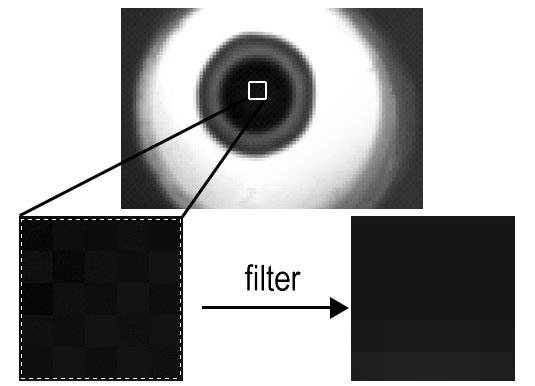
\includegraphics[width=0.5\linewidth]{Figures/4.Chapter/chess2.png}\\
\subfigure{
\begin{tikzpicture}
\begin{axis}[
	width=0.5\linewidth,
    height=0.3\linewidth,
	%title = {Unprocessed Results},
    tick label style={font=\scriptsize},
    legend style={font=\scriptsize,/tikz/column 2/.style={column sep=5pt},},
    %legend columns=2,
    legend cell align=left,
	legend pos =south east,
    grid=major, % Display a grid
    grid style={dashed,gray!30}, % Set the style
    xlabel={pixel},
    ylabel={T (ºC)}, 
    %ymin = 0, ymax = 11200,
    %ytick={300,325,350,375,400,425,450,475,500,525},
    %yticklabels={300,325,350,375,400,425,450,475,500,525},
    %xmin = 400, xmax = 1500,
    %ytick={0,1600,...,11200},
    %yticklabel style={
    %    /pgf/number format/fixed,
    %    /pgf/number format/precision=5},
	%scaled y ticks=false,
    ]
\addplot+[mark=square*,blue]
coordinates {(	1	,	29.23	)
(	2	,	32	)
(	3	,	32.7	)
(	4	,	34.09	)
(	5	,	33.05	)
(	6	,	34.09	)
(	7	,	32.7	)
(	8	,	34.09	)
(	9	,	34.09	)
(	10	,	37.9	)
(	11	,	41.03	)
(	12	,	44.84	)
(	13	,	44.15	)
(	14	,	43.45	)
(	15	,	40.33	)
};
%\addlegendentry{}
\end{axis}
\end{tikzpicture}
}%
\subfigure{
\begin{tikzpicture}
\begin{axis}[
	width=0.5\linewidth,
    height=0.3\linewidth,
	%title = {Processed Results},
    tick label style={font=\scriptsize},
    legend style={font=\scriptsize,/tikz/column 2/.style={column sep=5pt},},
    %legend columns=2,
    legend cell align=left,
	legend pos =south east,
    grid=major, % Display a grid
    grid style={dashed,gray!30}, % Set the style
    xlabel={pixel},
    ylabel={T (ºC)}, 
    %ymin = 0, ymax = 11200,
    %ytick={300,325,350,375,400,425,450,475,500,525},
    %yticklabels={300,325,350,375,400,425,450,475,500,525},
    %xmin = 400, xmax = 1500,
    %ytick={0,1600,...,11200},
    %yticklabel style={
    %    /pgf/number format/fixed,
    %    /pgf/number format/precision=5},
	%scaled y ticks=false,
    ]
\addplot+[mark=square*,blue]
coordinates {(	1	,	29.73	)
(	2	,	31.5	)
(	3	,	33.2	)
(	4	,	33.59	)
(	5	,	33.55	)
(	6	,	33.59	)
(	7	,	33.2	)
(	8	,	33.59	)
(	9	,	34.59	)
(	10	,	37.4	)
(	11	,	41.53	)
(	12	,	44.34	)
(	13	,	44.65	)
(	14	,	42.95	)
(	15	,	40.83	)
};
%\addlegendentry{}
\end{axis}
\end{tikzpicture}
}
\caption{Chess pattern example}
\label{fig:chess}
\end{figure}


\subsection{Median Filter}

\par This filter has the potential to remove random bad pixels noise from the picture. This filter is a MATLAB function that outputs the median of a 3-by-3 neighborhood of the input pixel. With this simple filter the image can be greatly improved as shown in Figure \ref{fig:median}. On the right there's the image without the filter and on the left the treated image.

\begin{figure}[h]
\centering

\includegraphics[width=0.6\linewidth]{Figures/4.Chapter/median.png}
\caption{Median filter effect}
\label{fig:median}
\end{figure}

\subsection{Background Filter}
\par The background filter serves the function of eliminating any problems related with the optics of the camera and to equalize the temperature field. Two different ways to do it were thought. Two MATLAB codes were made and tested. The first one is the simple way and is shown in Equation \ref{eq:bkg}. The variable $vid$ is the matrix with the temperature value for every pixel in every frame, $avTemp$ is the average temperature in the center of the hole and $t_n$ is the number of the analyzed frame.
\begin{equation}\label{eq:bkg}
vid^{*}(x,y,t_n)=vid(x,y,t_n)-vid(x,y,1)+avTemp
\end{equation}
\par The second one is a weighted background removal and we can see it in Equation \ref{eq:pbkg}. The variables bear the same meaning, but has to be done for each pixel ($x_p,y_p$). Only the code for the latter can be seen in Appendix \ref{ap:b} as the code is similar in both cases. 
\begin{equation}\label{eq:pbkg}
vid^{*}(x_p,y_p,t_n)=\frac{vid(x_p,y_p,t_n)-vid(x_p,y_p,1)}{vid(x_p,y_p,1)}avTemp+avTemp
\end{equation}
\begin{figure}[h]
\centering
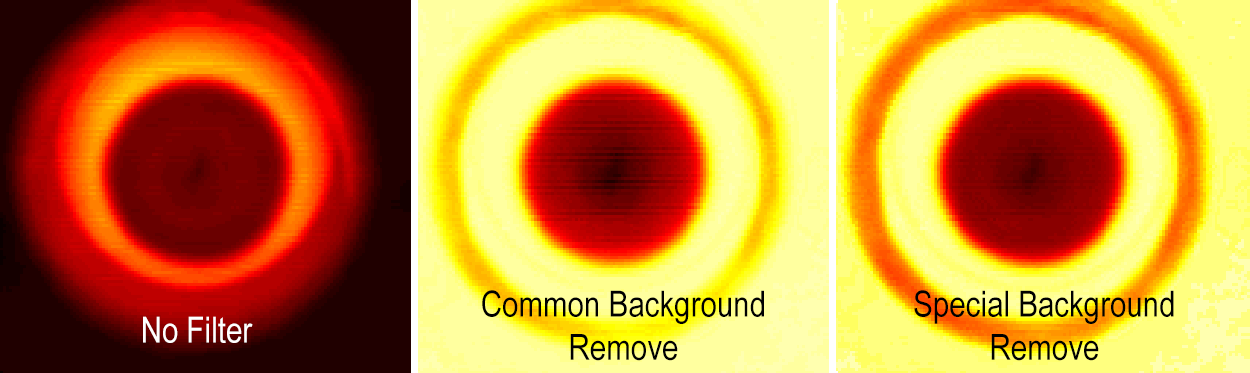
\includegraphics[width=0.8\linewidth]{Figures/4.Chapter/bkg.png}
\caption{Background filter effect}
\label{fig:bkg}
\end{figure}

\subsection{Heat Flux computation}

\par To evaluate and compare the heat removal capacity of the system it is very important to compute the heat flux and cooling effectiveness, mentioned in Section \ref{sec:heat}. This was also made with the help of a MATLAB code, that can be seen in Appendix \ref{ap:c} and \ref{ap:d}.\\
\par Starting with the computation of the


\cleardoublepage
\chapter{Experimental Results}
\label{cap:results}

\textit{In this chapter the experimental results will be shown and analyzed.}


\section{Horizontal Droplet View}

\par This experiment served as an initiation to the camera use. As stated before, the geometric implications of the droplet shape in radiation prevent the extraction of quantitative results.\\
\par This experiment was made in two different speeds: 2 m/s and 0.8 m/s, and three temperatures: 60ºC, 100ºC and 110ºC. A sample of the results of this experiment can be seen in Figure \ref{fig:hexp}. In this figure, the x axis represents the distance between the bottom of the droplet to its top. These results show that within the same speed, the temperature gradient evolves similarly between different temperatures, along the time. It is also noticeable the high temperature in the interface and the considerably lower temperature at the top.

\begin{figure}[h]
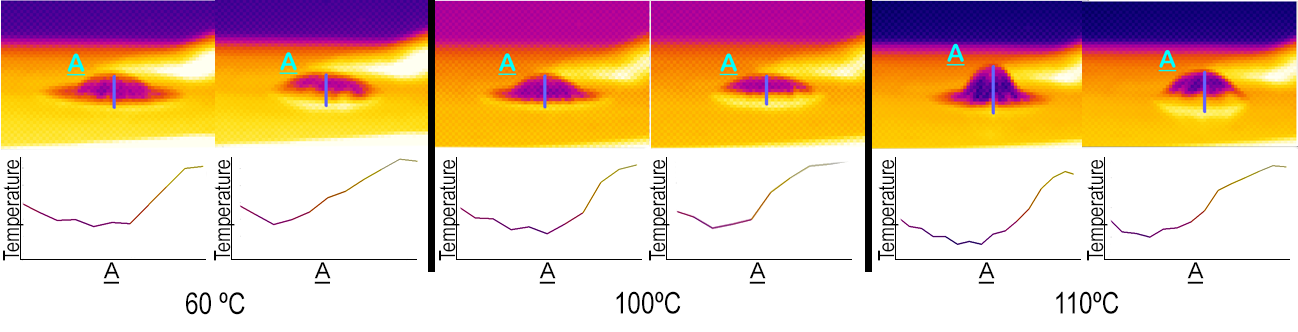
\includegraphics[width=1\linewidth]{Figures/5.Chapter/hexp.png}
\caption{Horizontal Results for 2 m/s during the spreading and receding phases}
\label{fig:hexp}
\end{figure}

\section{Bottom View}

\par The shown results will have a similar structure. Reading through this section, it is important to bear in mind that the results shown for a certain experiment can have both a bidimensional temperature map and a plot with temperatures along the radius for certain time-frames. The relation between the temperature maps, plots and the real image can be seen in Figure 

\begin{figure}[h]
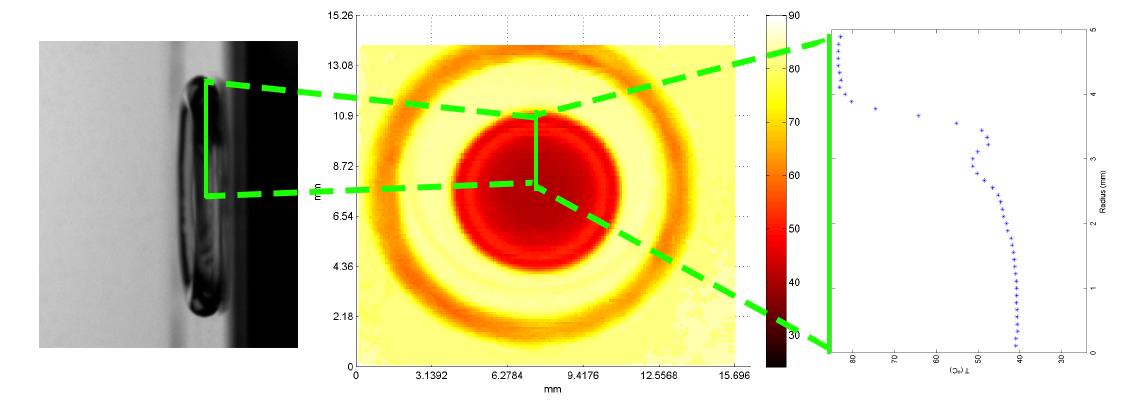
\includegraphics[width=1\linewidth]{Figures/5.Chapter/example.png}
\caption{Example of the results representation}
\label{fig:hexp}
\end{figure}

\par In the Bottom View experimental setup, various conditions were tested. Two different impact velocity values, with different characteristics: 0.8 m/s and 2 m/s. Four initial foil temperature values, representing conditions before and after saturation: 60ºC, 80ºC, 100ºC and 110ºC. Two different wettability, hydrophilic and hydrophobic, surfaces were tested. Finally, tests were also made with two liquids: water and ethanol. For each of the conditions, 5 different experiments were made, so that the repeatability of the tests could be confirmed. In Figure \ref{fig:repeat} the repeatability of these tests can be seen with the example of the 60ºC results for 2 m/s.\\

\begin{figure}
\centering
\begin{tikzpicture}
\begin{axis}[
	title = {2 m/s || 60 ºC || $T_{amb}=24$},
    tick label style={font=\scriptsize},
    legend style={font=\scriptsize,/tikz/column 2/.style={column sep=5pt},},
    %legend columns=2,
    legend cell align=left,
	legend pos =south east,
    grid=major, % Display a grid
    grid style={dashed,gray!30}, % Set the style
    xlabel={Droplet Radius (mm)},
    ylabel={T (ºC)}, 
    ymin = 25, ymax = 65,
    ytick={30,35,...,120},
    %yticklabels={300,325,350,375,400,425,450,475,500,525},
    xmin = 0, xmax = 7,
    %ytick={0,1600,...,11200},
    %yticklabel style={
    %    /pgf/number format/fixed,
    %    /pgf/number format/precision=5},
	%scaled y ticks=false,
    width=1\textwidth, 
    height=7cm,
    cycle list name= color
    ]
\addplot+[dashed]
coordinates {(	0	,	30.48	)
(	0.11	,	29.97	)
(	0.22	,	29.97	)
(	0.33	,	30.13	)
(	0.45	,	30.04	)
(	0.56	,	29.96	)
(	0.67	,	30.27	)
(	0.78	,	30.27	)
(	0.89	,	30.11	)
(	1	,	30.02	)
(	1.11	,	30.25	)
(	1.23	,	30.25	)
(	1.34	,	30.17	)
(	1.45	,	30.17	)
(	1.56	,	30.17	)
(	1.67	,	30.48	)
(	1.78	,	30.48	)
(	1.89	,	30.56	)
(	2.01	,	31.11	)
(	2.12	,	31.11	)
(	2.23	,	31.11	)
(	2.34	,	31.66	)
(	2.45	,	31.66	)
(	2.56	,	31.66	)
(	2.67	,	32.04	)
(	2.79	,	32.31	)
(	2.9	,	32.4	)
(	3.01	,	32.68	)
(	3.12	,	33.06	)
(	3.23	,	33.35	)
(	3.34	,	33.45	)
(	3.45	,	34.03	)
(	3.57	,	34.13	)
(	3.68	,	34.62	)
(	3.79	,	34.83	)
(	3.9	,	35.28	)
(	4.01	,	35.39	)
(	4.12	,	35.74	)
(	4.24	,	35.97	)
(	4.35	,	36.34	)
(	4.46	,	36.99	)
(	4.57	,	37.52	)
(	4.68	,	37.66	)
(	4.79	,	38.36	)
(	4.9	,	39.07	)
(	5.02	,	39.94	)
(	5.13	,	41.25	)
(	5.24	,	42.58	)
(	5.35	,	44.15	)
(	5.46	,	46.12	)
(	5.57	,	48.7	)
(	5.68	,	50.53	)
(	5.8	,	53.67	)
(	5.91	,	55.05	)
(	6.02	,	56.94	)
(	6.13	,	57.86	)
(	6.24	,	59.17	)
(	6.35	,	59.83	)
};
\addlegendentry{44 ms - exp 1}

\addplot+[dashed]
coordinates {(	0	,	29.18	)
(	0.11	,	28.88	)
(	0.22	,	28.81	)
(	0.33	,	28.73	)
(	0.44	,	28.9	)
(	0.55	,	29.28	)
(	0.66	,	29.58	)
(	0.77	,	29.36	)
(	0.88	,	29.29	)
(	0.99	,	29.22	)
(	1.11	,	29.15	)
(	1.22	,	29.38	)
(	1.33	,	29.31	)
(	1.44	,	29.24	)
(	1.55	,	29.17	)
(	1.66	,	29.53	)
(	1.77	,	29.66	)
(	1.88	,	29.73	)
(	1.99	,	29.8	)
(	2.1	,	30.16	)
(	2.21	,	30.66	)
(	2.32	,	30.58	)
(	2.43	,	30.58	)
(	2.54	,	30.93	)
(	2.65	,	31.08	)
(	2.76	,	31.31	)
(	2.87	,	31.31	)
(	2.98	,	31.47	)
(	3.09	,	31.78	)
(	3.2	,	31.78	)
(	3.32	,	32.39	)
(	3.43	,	32.83	)
(	3.54	,	33.18	)
(	3.65	,	33.27	)
(	3.76	,	33.82	)
(	3.87	,	34.28	)
(	3.98	,	34.67	)
(	4.09	,	35.24	)
(	4.2	,	35.67	)
(	4.31	,	35.67	)
(	4.42	,	36.22	)
(	4.53	,	36.57	)
(	4.64	,	37.31	)
(	4.75	,	37.81	)
(	4.86	,	38.72	)
(	4.97	,	39.67	)
(	5.08	,	41.03	)
(	5.19	,	42.81	)
(	5.3	,	44.63	)
(	5.42	,	46.87	)
(	5.53	,	49.15	)
(	5.64	,	51.83	)
(	5.75	,	54.13	)
(	5.86	,	56.06	)
(	5.97	,	58.19	)
(	6.08	,	59.43	)
(	6.19	,	60.02	)
(	6.3	,	59.89	)
};
\addlegendentry{44 ms - exp 2}

\addplot+[dashed]
coordinates {(	0	,	28.54	)
(	0.11	,	28.54	)
(	0.22	,	28.39	)
(	0.33	,	28.24	)
(	0.44	,	28.56	)
(	0.55	,	28.56	)
(	0.66	,	28.49	)
(	0.77	,	28.42	)
(	0.89	,	28.34	)
(	1	,	28.74	)
(	1.11	,	28.59	)
(	1.22	,	28.98	)
(	1.33	,	28.98	)
(	1.44	,	28.98	)
(	1.55	,	29.36	)
(	1.66	,	29.21	)
(	1.77	,	29.73	)
(	1.88	,	29.73	)
(	1.99	,	29.81	)
(	2.1	,	29.81	)
(	2.21	,	29.96	)
(	2.32	,	30.41	)
(	2.44	,	30.49	)
(	2.55	,	30.57	)
(	2.66	,	30.73	)
(	2.77	,	30.98	)
(	2.88	,	31.44	)
(	2.99	,	31.53	)
(	3.1	,	31.99	)
(	3.21	,	32.17	)
(	3.32	,	32.82	)
(	3.43	,	32.82	)
(	3.54	,	33.48	)
(	3.65	,	33.58	)
(	3.76	,	33.78	)
(	3.87	,	34.47	)
(	3.98	,	34.68	)
(	4.1	,	35.23	)
(	4.21	,	35.34	)
(	4.32	,	35.69	)
(	4.43	,	36.04	)
(	4.54	,	36.81	)
(	4.65	,	37.2	)
(	4.76	,	38	)
(	4.87	,	38.57	)
(	4.98	,	39.57	)
(	5.09	,	41.19	)
(	5.2	,	42.7	)
(	5.31	,	44.87	)
(	5.42	,	46.66	)
(	5.53	,	49.24	)
(	5.65	,	51.45	)
(	5.76	,	53.6	)
(	5.87	,	55.9	)
(	5.98	,	57.78	)
(	6.09	,	58.42	)
(	6.2	,	59.75	)
(	6.31	,	58.82	)
};
\addlegendentry{44 ms - exp 3}

\addplot+[dashed]
coordinates {(	0	,	28.24	)
(	0.11	,	28.1	)
(	0.22	,	28.03	)
(	0.33	,	27.96	)
(	0.44	,	27.96	)
(	0.55	,	27.82	)
(	0.66	,	27.82	)
(	0.77	,	27.76	)
(	0.88	,	27.76	)
(	0.99	,	28.01	)
(	1.1	,	27.94	)
(	1.21	,	28.31	)
(	1.32	,	28.62	)
(	1.43	,	28.62	)
(	1.54	,	28.62	)
(	1.65	,	28.75	)
(	1.76	,	28.82	)
(	1.87	,	29.41	)
(	1.98	,	29.41	)
(	2.09	,	29.41	)
(	2.2	,	29.77	)
(	2.31	,	29.99	)
(	2.42	,	30.07	)
(	2.53	,	30.3	)
(	2.63	,	30.69	)
(	2.74	,	30.69	)
(	2.85	,	30.69	)
(	2.96	,	31.32	)
(	3.07	,	31.69	)
(	3.18	,	31.86	)
(	3.29	,	32.04	)
(	3.4	,	32.68	)
(	3.51	,	33.06	)
(	3.62	,	33.25	)
(	3.73	,	33.65	)
(	3.84	,	34.24	)
(	3.95	,	34.94	)
(	4.06	,	35.28	)
(	4.17	,	35.62	)
(	4.28	,	35.97	)
(	4.39	,	36.47	)
(	4.5	,	36.85	)
(	4.61	,	37.66	)
(	4.72	,	37.93	)
(	4.83	,	39.07	)
(	4.94	,	40.1	)
(	5.05	,	41.42	)
(	5.16	,	42.76	)
(	5.27	,	44.73	)
(	5.38	,	47.33	)
(	5.49	,	49.39	)
(	5.6	,	51.78	)
(	5.71	,	54.49	)
(	5.82	,	56.12	)
(	5.93	,	57.8	)
(	6.04	,	59.48	)
(	6.15	,	59.31	)
(	6.26	,	58.69	)
};
\addlegendentry{44 ms - exp 4}

\addplot+[dashed]
coordinates {(	0	,	30.11	)
(	0.11	,	29.58	)
(	0.22	,	29.5	)
(	0.33	,	29.41	)
(	0.44	,	29.58	)
(	0.55	,	29.58	)
(	0.66	,	29.41	)
(	0.77	,	29.24	)
(	0.88	,	29.66	)
(	0.99	,	29.57	)
(	1.1	,	29.49	)
(	1.21	,	29.33	)
(	1.32	,	29.65	)
(	1.43	,	29.65	)
(	1.54	,	29.49	)
(	1.65	,	29.81	)
(	1.76	,	30.2	)
(	1.87	,	30.2	)
(	1.98	,	30.2	)
(	2.09	,	30.28	)
(	2.2	,	30.75	)
(	2.31	,	30.84	)
(	2.42	,	30.92	)
(	2.53	,	30.92	)
(	2.64	,	31.31	)
(	2.75	,	31.39	)
(	2.86	,	31.39	)
(	2.97	,	31.57	)
(	3.08	,	32.04	)
(	3.19	,	32.22	)
(	3.3	,	32.61	)
(	3.41	,	32.79	)
(	3.52	,	33.37	)
(	3.63	,	33.47	)
(	3.74	,	33.57	)
(	3.85	,	33.77	)
(	3.95	,	34.47	)
(	4.06	,	34.57	)
(	4.17	,	34.9	)
(	4.28	,	35.13	)
(	4.39	,	35.87	)
(	4.5	,	35.98	)
(	4.61	,	36.35	)
(	4.72	,	37	)
(	4.83	,	37.79	)
(	4.94	,	38.46	)
(	5.05	,	39.67	)
(	5.16	,	41.06	)
(	5.27	,	42.71	)
(	5.38	,	45.12	)
(	5.49	,	46.97	)
(	5.6	,	49.35	)
(	5.71	,	51.63	)
(	5.82	,	54.3	)
(	5.93	,	56.69	)
(	6.04	,	58.2	)
(	6.15	,	59.39	)
(	6.26	,	60.66	)
};
\addlegendentry{44 ms - exp 5}
\end{axis}
\end{tikzpicture}
\caption{Repeatability of the experiments}
\label{fig:repeat}
\end{figure}

\subsection{Before the Calibration}

\par Before the calibration method was used, some preliminary results were taken for comparison. To evaluate the quality of the calibration it is important to compare the results and interpret the differences. The same results were taken from the experiments before the calibration, than after the calibration. For the speeds of 2 m/s and 0.8 m/s, the foil temperatures of 60ºC, 100ºC and 110ºC were analyzed. A sample taken of the results before and after the applied method can be seen in Figure \ref{fig:calibcomp2}. \\

\par Before comparing the images, one should bare in mind the differences in their conditions. The results before calibration were taken at a different ambient temperature, and framerate. The average framerate of the results before the calibration is 990 fps, and 1100 after. One can only compare similar frames and differences may be accentuated by that. \\
\par One important aspect is that the diameter is approximately the same, which means that the droplets we can see, during the spreading phase (all the points before 23 ms) the new calibration and method captures a bit of the air trapping effect mentioned previously in Section \ref{sec:heat}, while this effect is not present in the results without the calibration. Another thing that was corrected, was the fact that the temperature would drop bellow the ambient temperature before the calibration. This is impossible because the droplet is at ambient temperature. The cause of this happening has roots on optical effects, that were nullified by the calibration. On the other side the calibrated camera results have some noise that couldn't be addressed without losing resolution. The cause of the noise is probably the improved installation that allowed for higher spatial resolution. So while there is advantages in the factory calibration, the proposed calibration can better portrait the physical phenomena. \\

\begin{figure}
\centering
\begin{tikzpicture}
\begin{axis}[
	title = {0.8 m/s || 107 ºC || $T_{amb}=21$},
    tick label style={font=\scriptsize},
    legend style={font=\scriptsize,/tikz/column 2/.style={column sep=5pt},},
    %legend columns=2,
    legend cell align=left,
	legend pos =south east,
    grid=major, % Display a grid
    grid style={dashed,gray!30}, % Set the style
    xlabel={Droplet Radius (mm)},
    ylabel={T (ºC)}, 
    ymin = 15, ymax = 125,
    ytick={20,40,...,120},
    %yticklabels={300,325,350,375,400,425,450,475,500,525},
    xmin = 0, xmax = 5,
    %ytick={0,1600,...,11200},
    %yticklabel style={
    %    /pgf/number format/fixed,
    %    /pgf/number format/precision=5},
	%scaled y ticks=false,
    width=0.5\textwidth, 
    height=7cm,
    cycle list name= color
    ]
\addplot+[dashed]
coordinates {(	0	,	87.65	)
(	0.19	,	90.34	)
(	0.385	,	93.17	)
(	0.575	,	96.69	)
(	0.765	,	101.8	)
(	0.955	,	105.96	)
(	1.15	,	106.32	)
(	1.34	,	106.96	)
(	1.53	,	107.37	)
(	1.72	,	107.37	)
(	1.915	,	107.37	)
(	2.105	,	107.37	)
(	2.295	,	107.37	)
(	2.485	,	107.37	)
(	2.68	,	107.37	)
(	2.87	,	107.37	)
(	3.06	,	107.19	)
(	3.25	,	107.37	)
(	3.445	,	107.37	)
(	3.635	,	107.55	)
(	3.825	,	107.37	)
(	4.015	,	107.37	)
(	4.21	,	107.37	)
(	4.4	,	107.37	)
(	4.59	,	107.37	)
};
\addlegendentry{1 ms}

\addplot+[dashed]
coordinates {(	0	,	56.42	)
(	0.19	,	57.47	)
(	0.385	,	57.65	)
(	0.575	,	59.29	)
(	0.765	,	60.71	)
(	0.955	,	62.4	)
(	1.15	,	64.4	)
(	1.34	,	68.33	)
(	1.53	,	74.09	)
(	1.72	,	78.19	)
(	1.915	,	82.3	)
(	2.105	,	86.82	)
(	2.295	,	94.22	)
(	2.485	,	104.08	)
(	2.68	,	106.32	)
(	2.87	,	107.37	)
(	3.06	,	107.19	)
(	3.25	,	107.37	)
(	3.445	,	106.96	)
(	3.635	,	107.37	)
(	3.825	,	107.37	)
(	4.015	,	107.19	)
(	4.21	,	107.37	)
(	4.4	,	107.37	)
(	4.59	,	107.37	)
};
\addlegendentry{3 ms}

\addplot+[dashed]
coordinates {(	0	,	37.93	)
(	0.19	,	38.57	)
(	0.385	,	38.52	)
(	0.575	,	38.75	)
(	0.765	,	38.75	)
(	0.955	,	38.75	)
(	1.15	,	37.93	)
(	1.34	,	38.57	)
(	1.53	,	39.98	)
(	1.72	,	44.91	)
(	1.915	,	53.13	)
(	2.105	,	59.88	)
(	2.295	,	59.88	)
(	2.485	,	58.29	)
(	2.68	,	58.88	)
(	2.87	,	61.35	)
(	3.06	,	78.84	)
(	3.25	,	101.62	)
(	3.445	,	105.72	)
(	3.635	,	106.73	)
(	3.825	,	107.37	)
(	4.015	,	106.96	)
(	4.21	,	107.37	)
(	4.4	,	106.96	)
(	4.59	,	107.37	)
};
\addlegendentry{7 ms}

\addplot+[dashed]
coordinates {(	0	,	29.07	)
(	0.19	,	30.35	)
(	0.385	,	30.12	)
(	0.575	,	30.12	)
(	0.765	,	29.71	)
(	0.955	,	29.53	)
(	1.15	,	28.89	)
(	1.34	,	30.12	)
(	1.53	,	33.41	)
(	1.72	,	40.39	)
(	1.915	,	45.32	)
(	2.105	,	46.14	)
(	2.295	,	42.86	)
(	2.485	,	39.8	)
(	2.68	,	40.39	)
(	2.87	,	47.61	)
(	3.06	,	68.33	)
(	3.25	,	90.93	)
(	3.445	,	102.85	)
(	3.635	,	105.9	)
(	3.825	,	106.78	)
(	4.015	,	106.55	)
(	4.21	,	106.96	)
(	4.4	,	106.96	)
(	4.59	,	107.37	)
};
\addlegendentry{13 ms}

\addplot+[dashed]
coordinates {(	0	,	20.67	)
(	0.19	,	23.13	)
(	0.385	,	24.78	)
(	0.575	,	26.24	)
(	0.765	,	26.01	)
(	0.955	,	26.42	)
(	1.15	,	26.6	)
(	1.34	,	29.3	)
(	1.53	,	32.17	)
(	1.72	,	35.05	)
(	1.915	,	34.82	)
(	2.105	,	34.82	)
(	2.295	,	34.82	)
(	2.485	,	37.52	)
(	2.68	,	42.86	)
(	2.87	,	53.95	)
(	3.06	,	69.39	)
(	3.25	,	85.59	)
(	3.445	,	97.51	)
(	3.635	,	103.44	)
(	3.825	,	105.72	)
(	4.015	,	106.14	)
(	4.21	,	106.96	)
(	4.4	,	106.96	)
(	4.59	,	107.37	)
};
\addlegendentry{23 ms}
\end{axis}
\end{tikzpicture}
\begin{tikzpicture}
\begin{axis}[
	title = {0.8 m/s || 117 ºC || $T_{amb}=24$},
    tick label style={font=\scriptsize},
    legend style={font=\scriptsize,/tikz/column 2/.style={column sep=5pt},},
    %legend columns=2,
    legend cell align=left,
	legend pos =south east,
    grid=major, % Display a grid
    grid style={dashed,gray!30}, % Set the style
    xlabel={Droplet Radius (mm)},
    ylabel={T (ºC)}, 
    ymin = 15, ymax = 125,
    ytick={20,40,...,120},
    %yticklabels={300,325,350,375,400,425,450,475,500,525},
    xmin = 0, xmax = 5,
    %ytick={0,1600,...,11200},
    %yticklabel style={
    %    /pgf/number format/fixed,
    %    /pgf/number format/precision=5},
	%scaled y ticks=false,
    width=0.5\textwidth, height=7cm,
    cycle list name= color
    ]
\addplot+[dashed]
coordinates {(	0	,	97.52	)
(	0.1	,	97.26	)
(	0.19	,	97.85	)
(	0.29	,	98.38	)
(	0.38	,	98.98	)
(	0.48	,	99.76	)
(	0.57	,	101.05	)
(	0.67	,	101.82	)
(	0.76	,	102.68	)
(	0.86	,	104.1	)
(	0.95	,	106.53	)
(	1.05	,	108.52	)
(	1.14	,	110.77	)
(	1.24	,	113.29	)
(	1.33	,	115.57	)
(	1.43	,	116.69	)
(	1.52	,	117.14	)
(	1.62	,	117.37	)
(	1.71	,	117.37	)
(	1.81	,	117.37	)
(	1.9	,	117.37	)
(	2	,	117.37	)
(	2.09	,	117.1	)
(	2.19	,	117.37	)
(	2.28	,	117.37	)
(	2.38	,	117.37	)
(	2.47	,	117.06	)
(	2.57	,	117.37	)
(	2.66	,	117.37	)
(	2.76	,	117.02	)
(	2.85	,	117.37	)
(	2.95	,	117.37	)
(	3.04	,	117.37	)
(	3.14	,	117.37	)
(	3.23	,	117.37	)
(	3.33	,	117.37	)
(	3.42	,	117.37	)
(	3.52	,	116.8	)
(	3.61	,	116.76	)
(	3.71	,	117.37	)
(	3.8	,	117.37	)
};
\addlegendentry{1 ms}

\addplot+[dashed]
coordinates {(	0	,	70.61	)
(	0.1	,	70.16	)
(	0.19	,	70.4	)
(	0.29	,	70.4	)
(	0.38	,	70.63	)
(	0.48	,	71.08	)
(	0.57	,	71.08	)
(	0.67	,	71.45	)
(	0.76	,	70.78	)
(	0.86	,	71.41	)
(	0.95	,	71.99	)
(	1.05	,	72.51	)
(	1.14	,	73.05	)
(	1.24	,	73.92	)
(	1.33	,	75.58	)
(	1.43	,	77.81	)
(	1.52	,	79.42	)
(	1.62	,	80.97	)
(	1.71	,	82.76	)
(	1.81	,	84.66	)
(	1.9	,	87.07	)
(	2	,	89.89	)
(	2.09	,	91.11	)
(	2.19	,	93.47	)
(	2.28	,	94.33	)
(	2.38	,	95.68	)
(	2.47	,	99.61	)
(	2.57	,	104.39	)
(	2.66	,	109.67	)
(	2.76	,	114.9	)
(	2.85	,	116.64	)
(	2.95	,	116.6	)
(	3.04	,	116.54	)
(	3.14	,	116.94	)
(	3.23	,	116.91	)
(	3.33	,	116.88	)
(	3.42	,	116.84	)
(	3.52	,	116.8	)
(	3.61	,	116.76	)
(	3.71	,	116.7	)
(	3.8	,	116.65	)
};
\addlegendentry{3 ms}

\addplot+[dashed]
coordinates {(	0	,	52.18	)
(	0.1	,	51.5	)
(	0.19	,	51.67	)
(	0.29	,	51.67	)
(	0.38	,	51.84	)
(	0.48	,	51.84	)
(	0.57	,	51.84	)
(	0.67	,	52.11	)
(	0.76	,	51.58	)
(	0.86	,	52.04	)
(	0.95	,	52.13	)
(	1.05	,	52.5	)
(	1.14	,	52.89	)
(	1.24	,	53.19	)
(	1.33	,	54.12	)
(	1.43	,	55.15	)
(	1.52	,	56.08	)
(	1.62	,	56.86	)
(	1.71	,	57.21	)
(	1.81	,	57.93	)
(	1.9	,	58.43	)
(	2	,	60.23	)
(	2.09	,	62.39	)
(	2.19	,	66.52	)
(	2.28	,	68.19	)
(	2.38	,	67.5	)
(	2.47	,	66.4	)
(	2.57	,	62.8	)
(	2.66	,	62.84	)
(	2.76	,	64.79	)
(	2.85	,	74.42	)
(	2.95	,	84.98	)
(	3.04	,	101.24	)
(	3.14	,	108.17	)
(	3.23	,	115.5	)
(	3.33	,	116.38	)
(	3.42	,	116.3	)
(	3.52	,	116.22	)
(	3.61	,	116.14	)
(	3.71	,	116.7	)
(	3.8	,	116.65	)
};
\addlegendentry{7 ms}

\addplot+[dashed]
coordinates {(	0	,	43.06	)
(	0.1	,	43.06	)
(	0.19	,	43.2	)
(	0.29	,	43.2	)
(	0.38	,	43.35	)
(	0.48	,	43.35	)
(	0.57	,	43.35	)
(	0.67	,	43.57	)
(	0.76	,	42.84	)
(	0.86	,	43.21	)
(	0.95	,	43.29	)
(	1.05	,	43.6	)
(	1.14	,	43.92	)
(	1.24	,	45.08	)
(	1.33	,	45.25	)
(	1.43	,	46.41	)
(	1.52	,	47.47	)
(	1.62	,	49	)
(	1.71	,	50.17	)
(	1.81	,	50.8	)
(	1.9	,	51.24	)
(	2	,	51.26	)
(	2.09	,	51.26	)
(	2.19	,	50.46	)
(	2.28	,	50.71	)
(	2.38	,	50.22	)
(	2.47	,	49.97	)
(	2.57	,	51.82	)
(	2.66	,	54.59	)
(	2.76	,	60.39	)
(	2.85	,	69.88	)
(	2.95	,	81.73	)
(	3.04	,	94.08	)
(	3.14	,	104.64	)
(	3.23	,	110.08	)
(	3.33	,	114.35	)
(	3.42	,	116.3	)
(	3.52	,	116.22	)
(	3.61	,	116.14	)
(	3.71	,	116.7	)
(	3.8	,	116.65	)
};
\addlegendentry{13 ms}

\addplot+[dashed]
coordinates {(	0	,	34.36	)
(	0.1	,	35.44	)
(	0.19	,	36.61	)
(	0.29	,	37.63	)
(	0.38	,	38.75	)
(	0.48	,	38.75	)
(	0.57	,	38.75	)
(	0.67	,	38.95	)
(	0.76	,	39.08	)
(	0.86	,	40.41	)
(	0.95	,	40.48	)
(	1.05	,	41.74	)
(	1.14	,	42.05	)
(	1.24	,	42.28	)
(	1.33	,	42.44	)
(	1.43	,	42.69	)
(	1.52	,	42.85	)
(	1.62	,	43.45	)
(	1.71	,	44.7	)
(	1.81	,	45.27	)
(	1.9	,	45.66	)
(	2	,	47.48	)
(	2.09	,	47.48	)
(	2.19	,	48.49	)
(	2.28	,	48.72	)
(	2.38	,	50.22	)
(	2.47	,	52	)
(	2.57	,	54.82	)
(	2.66	,	58.44	)
(	2.76	,	64.79	)
(	2.85	,	72.95	)
(	2.95	,	81.73	)
(	3.04	,	91.1	)
(	3.14	,	99.25	)
(	3.23	,	104.75	)
(	3.33	,	111.74	)
(	3.42	,	115.21	)
(	3.52	,	115.63	)
(	3.61	,	116.14	)
(	3.71	,	116.7	)
(	3.8	,	116.65	)
};
\addlegendentry{23 ms}
\end{axis}
\end{tikzpicture}
\caption{Comparison between results with and without the proposed calibration}
\label{fig:calibcomp2}
\end{figure}

\section{Bottom View - Temperature results vs High Speed results}

\begin{figure}
\centering
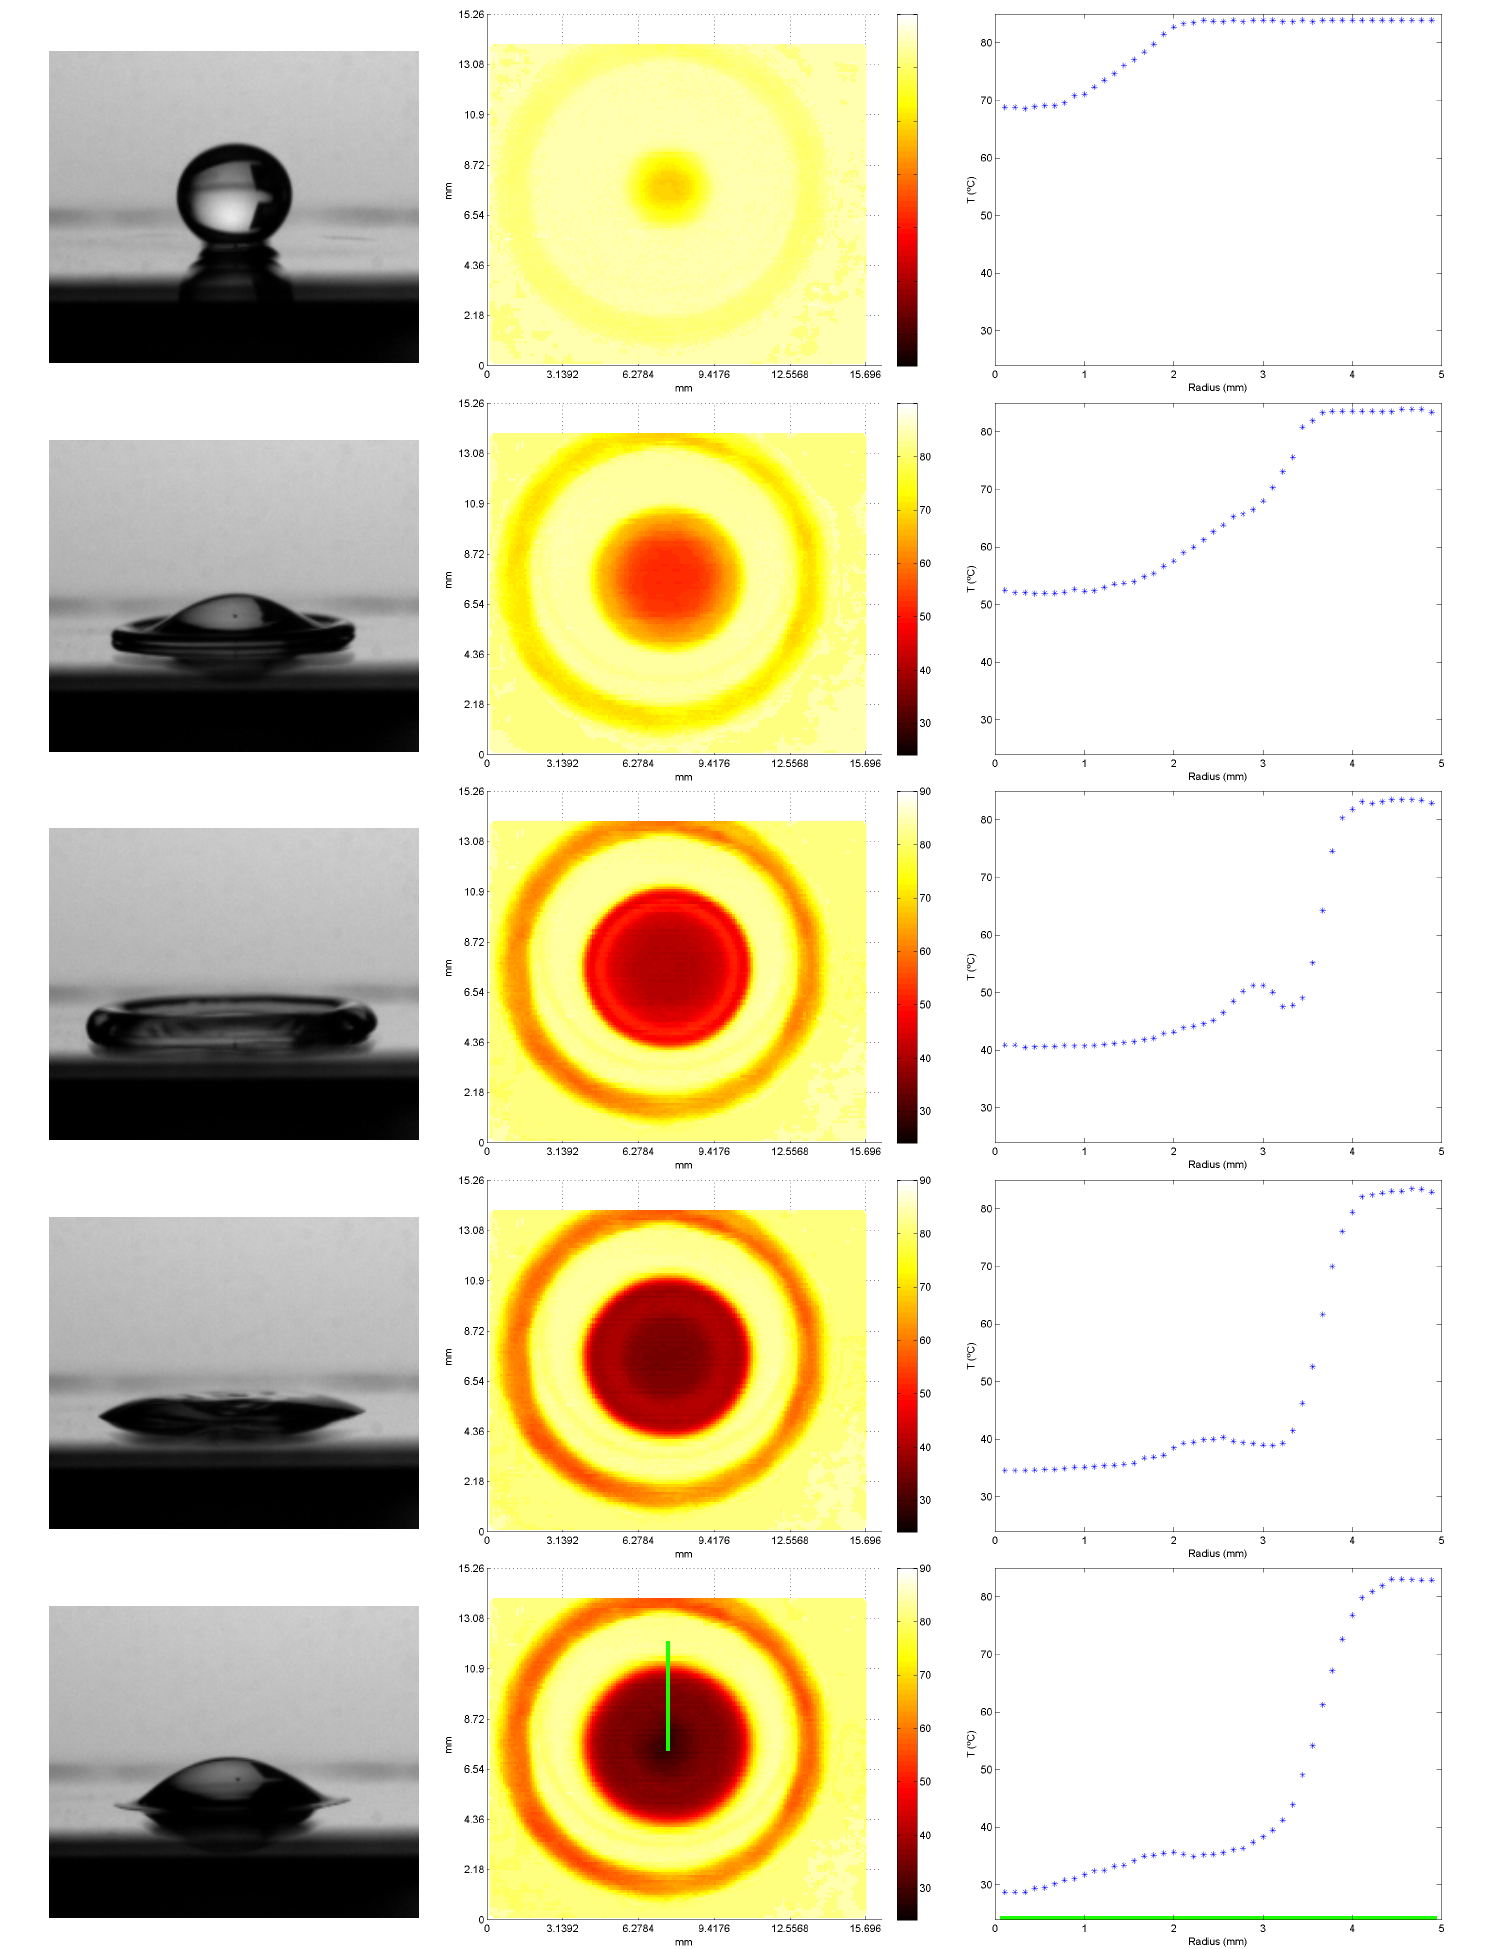
\includegraphics[width=1\linewidth]{Figures/5.Chapter/IRvsHR.png}
\caption{Comparison between High Speed camera images and Infra Red images for 0.8m/s and 80ºC at 0, 2, 6, 12 and 22 ms after the first contact on a hydrophilic surface}
\label{fig:irvshr}
\end{figure}

\par One important objective of this work is to use the high-speed camera to compare physical phenomena with thermal phenomena. The results were put together in Figure \ref{fig:irvshr}. In this figure it is possible to see some of the stages of a droplet impact. Analyzing the images, it's observable the physical phenomena that have an impact on heat transfer. During the spreading, the interior ring in the temperature maps, presented in the third and fourth images, reflect the presence of the wave formed during the spreading. When this wave reaches maximum diameter it reverses in the recoiling phase. The thickness of the water layer is smaller right before the wave. In this area there is less heat removal. So, as expected, one can see a ring of higher temperatures, and a slope in the plot. After the recoiling phase the droplet starts to stabilize, and due to it's hemispherical shape the heat flux is higher at the center, so the temperature is lower in the center.

\subsection{Velocity Influence}

\par For an hidrophilic surface, results were taken for different velocities: 0.8 m/s, 2 m/s. The obvious difference is in the spreading diameter, which is directly influenced by the impact velocity. This can be seen in Figure \label{fig:irvshr}. One of the differences is the fingering, that only happens for 2 m/s (at t= 6ms). The height of the lamela is also smaller for this velocity.

\begin{figure}[h]
\centering
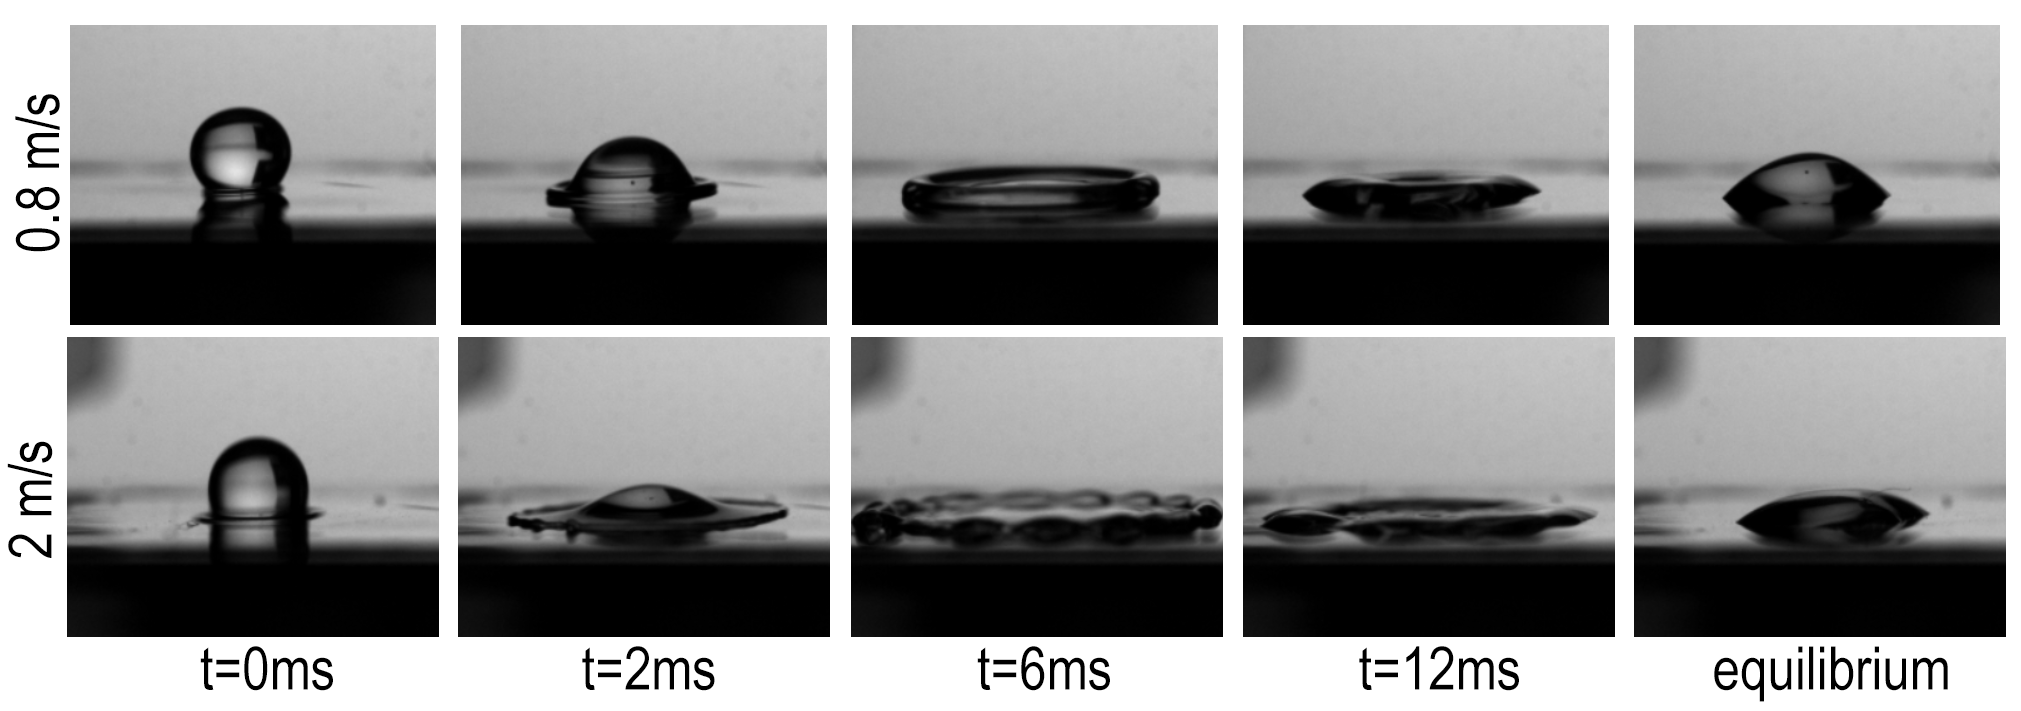
\includegraphics[width=1\linewidth]{Figures/5.Chapter/hsspeed.png}
\caption{Velocity HS images comparison for a hydrophilic surface at 100ºC}
\label{fig:irvshr}
\end{figure}


\par Using the high speed camera it was possible to extract the droplet diameter for each frame, with the help of a code developed previously by Tomás Valente. The comparison between the spreading factor of each velocity can be seen in Figure \ref{fig:diameter}. As expected the spreading factor grows more with a higher impact velocity.

\begin{figure}[h]
\centering
\begin{tikzpicture}
\begin{axis}[
	title = {Spreading Diameter},
    tick label style={font=\scriptsize},
    legend style={font=\scriptsize,/tikz/column 2/.style={column sep=5pt},},
    %legend columns=2,
    legend cell align=left,
	legend pos =south east,
    grid=major, % Display a grid
    grid style={dashed,gray!30}, % Set the style
    xlabel={Time (s)},
    ylabel={Spreading Factor}, 
    ymin = 0, ymax = 4.5,
    ytick={0,0.5,...,4.5},
    %yticklabels={300,325,350,375,400,425,450,475,500,525},
    xmin = 0, xmax = 0.025,
    %ytick={0,1600,...,11200},
    %yticklabel style={
    %    /pgf/number format/fixed,
    %    /pgf/number format/precision=5},
	%scaled y ticks=false,
    width=1\textwidth, height=5cm,
    cycle list name= color
    ]
\addplot+[dashed]
coordinates {(	0	,	0.515151515	)
(	0.000454545	,	1.939393939	)
(	0.000909091	,	2.636363636	)
(	0.001363636	,	3.015151515	)
(	0.001818182	,	3.363636364	)
(	0.002272727	,	3.545454545	)
(	0.002727273	,	3.712121212	)
(	0.003181818	,	3.787878788	)
(	0.003636364	,	3.833333333	)
(	0.004090909	,	3.863636364	)
(	0.004545455	,	3.848484848	)
(	0.005	,	3.818181818	)
(	0.005454545	,	3.818181818	)
(	0.005909091	,	3.833333333	)
(	0.006363636	,	3.772727273	)
(	0.006818182	,	3.757575758	)
(	0.007272727	,	3.772727273	)
(	0.007727273	,	3.681818182	)
(	0.008181818	,	3.696969697	)
(	0.008636364	,	3.621212121	)
(	0.009090909	,	3.621212121	)
(	0.01	,	3.53030303	)
(	0.010909091	,	3.454545455	)
(	0.011818182	,	3.393939394	)
(	0.012727273	,	3.318181818	)
(	0.013636364	,	3.242424242	)
(	0.014545455	,	3.106060606	)
(	0.015454545	,	3.090909091	)
(	0.019090909	,	2.818181818	)
(	0.022727273	,	2.636363636	)
};
\addlegendentry{2 m/s}

\addplot+[dashed]
coordinates {(	0	,	0.166303558	)
(	0.000454545	,	0.680332739	)
(	0.000909091	,	1.179243415	)
(	0.001363636	,	1.602561563	)
(	0.001818182	,	1.889813164	)
(	0.002272727	,	2.131709249	)
(	0.002727273	,	2.298012808	)
(	0.003181818	,	2.403842345	)
(	0.003636364	,	2.479434872	)
(	0.004090909	,	2.539908893	)
(	0.004545455	,	2.570145903	)
(	0.005	,	2.585264409	)
(	0.005454545	,	2.585264409	)
(	0.005909091	,	2.585264409	)
(	0.006363636	,	2.585264409	)
(	0.006818182	,	2.570145903	)
(	0.007272727	,	2.570145903	)
(	0.007727273	,	2.555027398	)
(	0.008181818	,	2.539908893	)
(	0.008636364	,	2.524790388	)
(	0.009090909	,	2.509671882	)
(	0.009545455	,	2.494553377	)
(	0.01	,	2.479434872	)
(	0.010454545	,	2.449197861	)
(	0.010909091	,	2.434079356	)
(	0.011363636	,	2.403842345	)
(	0.011818182	,	2.38872384	)
(	0.012272727	,	2.373605334	)
(	0.012727273	,	2.343368324	)
(	0.013181818	,	2.343368324	)
(	0.013636364	,	2.313131313	)
(	0.014090909	,	2.282894303	)
(	0.014545455	,	2.282894303	)
(	0.015	,	2.252657292	)
(	0.015454545	,	2.237538787	)
(	0.015909091	,	2.222420281	)
(	0.016363636	,	2.207301776	)
(	0.016818182	,	2.177064765	)
(	0.017272727	,	2.16194626	)
(	0.017727273	,	2.16194626	)
(	0.018181818	,	2.146827755	)
(	0.018636364	,	2.131709249	)
(	0.019090909	,	2.131709249	)
(	0.019545455	,	2.116590744	)
(	0.02	,	2.101472239	)
(	0.020454545	,	2.101472239	)
(	0.020909091	,	2.071235228	)
(	0.021363636	,	2.071235228	)
(	0.021818182	,	2.056116723	)
(	0.022272727	,	2.040998217	)
(	0.022727273	,	2.025879712	)
};
\addlegendentry{0.8 m/s}

\end{axis}
\end{tikzpicture}
\caption{Comparison between the spreading factor of each velocity}
\label{fig:diameter}
\end{figure}

\par Lets now take a look at the influence of the velocity in the temperature field. In Figure \ref{fig:speed1}, the average of all experiments made for both velocity values at 100ºC is presented for comparison. The temperature at the center of the droplet is similar during the spreading (3ms and 13 ms). The temperature at the droplet center drops more intensely in the lower velocity. This is justified by the height difference, also noticeable in the last panel of Figure \ref{fig:irvshr}. Looking at the shape of the curves, one can observe their similarity. This may be a signal of the time in which the phenomena occur is mostly independent of the impact velocity. Note that the curves have close temperatures in the center area and also that the lower velocity tests show always higher temperatures at the same point than the higher velocity ones outside the center. With this in mind, it's safe to assume that the higher velocity droplet removed more heat from the foil.

\begin{figure}[h]
\centering
\begin{tikzpicture}
\begin{axis}[
	%title = {107 ºC || $T_{amb}=24$},
    tick label style={font=\scriptsize},
    legend style={font=\scriptsize,/tikz/column 2/.style={column sep=5pt},},
    %legend columns=2,
    legend cell align=left,
	legend pos =south east,
    grid=major, % Display a grid
    grid style={dashed,gray!30}, % Set the style
    xlabel={Droplet Radius (mm)},
    ylabel={T (ºC)}, 
    ymin = 55, ymax = 113,
    ytick={60,70,...,100,110},
    %yticklabels={300,325,350,375,400,425,450,475,500,525},
    xmin = 0, xmax = 7,
    %ytick={0,1600,...,11200},
    %yticklabel style={
    %    /pgf/number format/fixed,
    %    /pgf/number format/precision=5},
	%scaled y ticks=false,
    width=1\textwidth, height=7cm,
    cycle list name= color
    ]
\addplot+[dashed]
coordinates {(	0	,	65.76	)
(	0.12	,	65.9	)
(	0.23	,	65.85	)
(	0.35	,	66.09	)
(	0.46	,	66.07	)
(	0.58	,	66.22	)
(	0.69	,	66.79	)
(	0.81	,	67.14	)
(	0.92	,	67.57	)
(	1.04	,	68.07	)
(	1.16	,	68.69	)
(	1.27	,	69.25	)
(	1.39	,	70.14	)
(	1.5	,	71.11	)
(	1.62	,	72.38	)
(	1.73	,	73.98	)
(	1.85	,	75.64	)
(	1.97	,	77.5	)
(	2.08	,	79.6	)
(	2.2	,	81.25	)
(	2.31	,	82.46	)
(	2.43	,	84	)
(	2.54	,	85.63	)
(	2.66	,	87.47	)
(	2.77	,	89.31	)
(	2.89	,	91.96	)
(	3.01	,	94.76	)
(	3.12	,	97.56	)
(	3.24	,	99.83	)
(	3.35	,	101.74	)
(	3.47	,	102.78	)
(	3.58	,	103.09	)
(	3.7	,	103.17	)
(	3.81	,	103.25	)
(	3.93	,	103.13	)
(	4.05	,	103.23	)
(	4.16	,	103.22	)
(	4.28	,	103.31	)
(	4.39	,	103.17	)
(	4.51	,	103.02	)
(	4.62	,	102.99	)
};
\addlegendentry{0.8 m/s - 3 ms}

\addplot+[dashed]
coordinates {(	0	,	64.76	)
(	0.12	,	64.97	)
(	0.23	,	64.61	)
(	0.35	,	64.44	)
(	0.46	,	64.13	)
(	0.58	,	64.08	)
(	0.69	,	64.09	)
(	0.81	,	63.56	)
(	0.92	,	63.26	)
(	1.04	,	63.34	)
(	1.16	,	63.22	)
(	1.27	,	63.12	)
(	1.39	,	63.12	)
(	1.5	,	62.93	)
(	1.62	,	63.29	)
(	1.73	,	63.7	)
(	1.85	,	63.88	)
(	1.97	,	64.17	)
(	2.08	,	64.58	)
(	2.2	,	65.21	)
(	2.31	,	65.97	)
(	2.43	,	66.51	)
(	2.54	,	67.27	)
(	2.66	,	68.47	)
(	2.77	,	69.17	)
(	2.89	,	70.41	)
(	3.01	,	71.01	)
(	3.12	,	72.19	)
(	3.24	,	73.14	)
(	3.35	,	73.85	)
(	3.47	,	74.52	)
(	3.58	,	75.4	)
(	3.7	,	76.25	)
(	3.81	,	77.3	)
(	3.93	,	78.35	)
(	4.05	,	79.18	)
(	4.16	,	80.08	)
(	4.28	,	81.21	)
(	4.39	,	82.8	)
(	4.51	,	84	)
(	4.62	,	85.5	)
(	4.74	,	87.06	)
(	4.85	,	89.03	)
(	4.97	,	90.91	)
(	5.09	,	93.49	)
(	5.2	,	96.19	)
(	5.32	,	100.05	)
(	5.43	,	103.28	)
(	5.55	,	105.25	)
(	5.66	,	106.11	)
(	5.78	,	106.44	)
(	5.9	,	106.29	)
(	6.01	,	106.37	)
(	6.13	,	106.42	)
(	6.24	,	106	)
(	6.36	,	105.96	)
(	6.47	,	105.78	)
(	6.59	,	105.59	)
};
\addlegendentry{2 m/s - 3 ms}

\end{axis}
\end{tikzpicture}
\begin{tikzpicture}
\begin{axis}[
	%title = {107 ºC || $T_{amb}=24$},
    tick label style={font=\scriptsize},
    legend style={font=\scriptsize,/tikz/column 2/.style={column sep=5pt},},
    %legend columns=2,
    legend cell align=left,
	legend pos =north west,
    grid=major, % Display a grid
    grid style={dashed,gray!30}, % Set the style
    xlabel={Droplet Radius (mm)},
    ylabel={T (ºC)}, 
    ymin = 35, ymax = 113,
    ytick={30,40,...,100,110},
    %yticklabels={300,325,350,375,400,425,450,475,500,525},
    xmin = 0, xmax = 7,
    %ytick={0,1600,...,11200},
    %yticklabel style={
    %    /pgf/number format/fixed,
    %    /pgf/number format/precision=5},
	%scaled y ticks=false,
    width=1\textwidth, height=7cm,
    cycle list name= color
    ]
\addplot+[dashed]
coordinates {(	0	,	40.31	)
(	0.12	,	40.55	)
(	0.23	,	40.46	)
(	0.35	,	40.67	)
(	0.46	,	40.82	)
(	0.58	,	40.91	)
(	0.69	,	41.1	)
(	0.81	,	41.36	)
(	0.92	,	41.52	)
(	1.04	,	41.6	)
(	1.16	,	41.71	)
(	1.27	,	42.12	)
(	1.39	,	42.45	)
(	1.5	,	42.66	)
(	1.62	,	43.31	)
(	1.73	,	43.95	)
(	1.85	,	45.07	)
(	1.97	,	45.77	)
(	2.08	,	46.81	)
(	2.2	,	47.54	)
(	2.31	,	48.29	)
(	2.43	,	49.09	)
(	2.54	,	49.17	)
(	2.66	,	49.05	)
(	2.77	,	48.75	)
(	2.89	,	48.29	)
(	3.01	,	48.6	)
(	3.12	,	49.5	)
(	3.24	,	51.61	)
(	3.35	,	56.13	)
(	3.47	,	61.63	)
(	3.58	,	68.59	)
(	3.7	,	76.42	)
(	3.81	,	84.29	)
(	3.93	,	91.67	)
(	4.05	,	96.84	)
(	4.16	,	100.05	)
(	4.28	,	101.53	)
(	4.39	,	102.28	)
(	4.51	,	102.08	)
(	4.62	,	101.62	)
};
\addlegendentry{0.8 m/s - 13 ms}

\addplot+[dashed]
coordinates {(	0	,	41.51	)
(	0.12	,	41.44	)
(	0.23	,	41.31	)
(	0.35	,	41.14	)
(	0.46	,	40.77	)
(	0.58	,	40.61	)
(	0.69	,	40.39	)
(	0.81	,	40.57	)
(	0.92	,	40.22	)
(	1.04	,	40.24	)
(	1.16	,	40.11	)
(	1.27	,	40.11	)
(	1.39	,	40.05	)
(	1.5	,	39.87	)
(	1.62	,	39.81	)
(	1.73	,	39.79	)
(	1.85	,	39.95	)
(	1.97	,	39.91	)
(	2.08	,	40.28	)
(	2.2	,	40.34	)
(	2.31	,	40.64	)
(	2.43	,	40.65	)
(	2.54	,	41.02	)
(	2.66	,	41.57	)
(	2.77	,	41.97	)
(	2.89	,	42.46	)
(	3.01	,	43.23	)
(	3.12	,	43.95	)
(	3.24	,	44.59	)
(	3.35	,	45.3	)
(	3.47	,	46.08	)
(	3.58	,	46.71	)
(	3.7	,	47.43	)
(	3.81	,	47.91	)
(	3.93	,	48.5	)
(	4.05	,	49.05	)
(	4.16	,	49.05	)
(	4.28	,	49.21	)
(	4.39	,	49.27	)
(	4.51	,	49.33	)
(	4.62	,	49.37	)
(	4.74	,	49.62	)
(	4.85	,	49.94	)
(	4.97	,	50.54	)
(	5.09	,	52.22	)
(	5.2	,	54.01	)
(	5.32	,	57.83	)
(	5.43	,	64.46	)
(	5.55	,	73.26	)
(	5.66	,	82.58	)
(	5.78	,	91.23	)
(	5.9	,	97.63	)
(	6.01	,	101.44	)
(	6.13	,	103.55	)
(	6.24	,	104.15	)
(	6.36	,	104.67	)
(	6.47	,	104.97	)
(	6.59	,	104.65	)
};
\addlegendentry{2 m/s - 13 ms}
\end{axis}
\end{tikzpicture}
\begin{tikzpicture}
\begin{axis}[
	%
    tick label style={font=\scriptsize},
    legend style={font=\scriptsize,/tikz/column 2/.style={column sep=5pt},},
    %legend columns=2,
    legend cell align=left,
	legend pos =north west,
    grid=major, % Display a grid
    grid style={dashed,gray!30}, % Set the style
    xlabel={Droplet Radius (mm)},
    ylabel={T (ºC)}, 
    ymin = 30, ymax = 113,
    ytick={30,40,...,100,110},
    %yticklabels={300,325,350,375,400,425,450,475,500,525},
    xmin = 0, xmax = 7,
    %ytick={0,1600,...,11200},
    %yticklabel style={
    %    /pgf/number format/fixed,
    %    /pgf/number format/precision=5},
	%scaled y ticks=false,
    width=1\textwidth, height=7cm,
    cycle list name= color
    ]
\addplot+[dashed]
coordinates {(	0	,	31.46	)
(	0.12	,	31.32	)
(	0.23	,	31.38	)
(	0.35	,	31.53	)
(	0.46	,	31.66	)
(	0.58	,	32.15	)
(	0.69	,	32.52	)
(	0.81	,	32.8	)
(	0.92	,	33.75	)
(	1.04	,	33.96	)
(	1.16	,	35	)
(	1.27	,	35.59	)
(	1.39	,	36.46	)
(	1.5	,	36.84	)
(	1.62	,	37.3	)
(	1.73	,	38.14	)
(	1.85	,	38.58	)
(	1.97	,	39.1	)
(	2.08	,	39.81	)
(	2.2	,	40.56	)
(	2.31	,	41.33	)
(	2.43	,	42.55	)
(	2.54	,	43.29	)
(	2.66	,	45.03	)
(	2.77	,	46.72	)
(	2.89	,	49.02	)
(	3.01	,	51.27	)
(	3.12	,	54.26	)
(	3.24	,	57.42	)
(	3.35	,	61.69	)
(	3.47	,	66.25	)
(	3.58	,	70.58	)
(	3.7	,	75.28	)
(	3.81	,	79.81	)
(	3.93	,	84.25	)
(	4.05	,	88.44	)
(	4.16	,	91.48	)
(	4.28	,	94.72	)
(	4.39	,	97	)
(	4.51	,	98.21	)
(	4.62	,	99.1	)
};
\addlegendentry{0.8 m/s - 54 ms}

\addplot+[dashed]
coordinates {(	0	,	35.05	)
(	0.12	,	34.63	)
(	0.23	,	34.58	)
(	0.35	,	34.24	)
(	0.46	,	34.48	)
(	0.58	,	34.4	)
(	0.69	,	34.56	)
(	0.81	,	34.42	)
(	0.92	,	34.26	)
(	1.04	,	34.72	)
(	1.16	,	34.6	)
(	1.27	,	35.17	)
(	1.39	,	35.31	)
(	1.5	,	35.71	)
(	1.62	,	35.84	)
(	1.73	,	36.19	)
(	1.85	,	36.73	)
(	1.97	,	37.22	)
(	2.08	,	37.44	)
(	2.2	,	37.85	)
(	2.31	,	38.32	)
(	2.43	,	38.85	)
(	2.54	,	39.73	)
(	2.66	,	40.45	)
(	2.77	,	41.01	)
(	2.89	,	41.65	)
(	3.01	,	42.6	)
(	3.12	,	43.01	)
(	3.24	,	43.82	)
(	3.35	,	44.37	)
(	3.47	,	44.7	)
(	3.58	,	45.48	)
(	3.7	,	45.91	)
(	3.81	,	46.53	)
(	3.93	,	47.14	)
(	4.05	,	47.55	)
(	4.16	,	47.86	)
(	4.28	,	48.81	)
(	4.39	,	49.67	)
(	4.51	,	50.37	)
(	4.62	,	51.56	)
(	4.74	,	52.65	)
(	4.85	,	54.44	)
(	4.97	,	56.31	)
(	5.09	,	58.93	)
(	5.2	,	62.17	)
(	5.32	,	65.89	)
(	5.43	,	70.41	)
(	5.55	,	74.98	)
(	5.66	,	79.66	)
(	5.78	,	84.19	)
(	5.9	,	88.29	)
(	6.01	,	92.34	)
(	6.13	,	95.38	)
(	6.24	,	96.93	)
(	6.36	,	98.86	)
(	6.47	,	101.02	)
(	6.59	,	102.02	)
};
\addlegendentry{2 m/s - 54 ms}

\end{axis}
\end{tikzpicture}
\caption{Average temperature along the radius between the 5 experiments of both velocity values at 100ºC}
\label{fig:speed1}
\end{figure}

\subsection{Temperature Influence}

\par This section will address the relative temperature drop in the foil for the tested temperatures. The temperatures had to be adimensionalized  so that they could be compared. \\

\par This analysis, for a fixed impact velocity of 0.8 m/s, can be seen in Figure \ref{fig:temp}. In this figure one can see that for the different initial temperatures, the relative temperature drop is very similar in the center, but has a significant difference in the edge area. This may be the cause of different diameters at that time, which can shift the curve.

\par This is a confirmation for the effectiveness of the  weighted background test. Because the curves vary so little for the different temperatures, one can assume that the relative temperature drop is constant and so, even if the background has different temperatures at its initial stage it is possible to assume a constant temperature if this technique is used.

\begin{figure}[h]
\centering
\begin{tikzpicture}
\begin{axis}[
	title = {0.8 m/s || 3ms},
    tick label style={font=\scriptsize},
    legend style={font=\scriptsize,/tikz/column 2/.style={column sep=5pt},},
    %legend columns=2,
    legend cell align=left,
	legend pos =south east,
    grid=major, % Display a grid
    grid style={dashed,gray!30}, % Set the style
    xlabel={Droplet Radius (mm)},
    ylabel={\LARGE{$\frac{T-T_{amb}}{T_{max}-T_{amb}}$}}, 
    ymin = 0, ymax = 1,
    ytick={0,0.1,...,1},
    %yticklabels={300,325,350,375,400,425,450,475,500,525},
    xmin = 0, xmax = 5,
    %ytick={0,1600,...,11200},
    %yticklabel style={
    %    /pgf/number format/fixed,
    %    /pgf/number format/precision=5},
	%scaled y ticks=false,
    width=1\textwidth, 
    height=7cm,
    cycle list name= color
    ]
\addplot+[dashed]
coordinates {(	0	,	0.514798887	)
(	0.11	,	0.515304832	)
(	0.22	,	0.514292942	)
(	0.33	,	0.511257273	)
(	0.44	,	0.508221604	)
(	0.55	,	0.509233494	)
(	0.65	,	0.511510245	)
(	0.76	,	0.51302808	)
(	0.87	,	0.514292942	)
(	0.98	,	0.517328611	)
(	1.09	,	0.519605363	)
(	1.2	,	0.518846446	)
(	1.31	,	0.519858335	)
(	1.42	,	0.523652922	)
(	1.53	,	0.532506957	)
(	1.64	,	0.544143688	)
(	1.75	,	0.560839868	)
(	1.86	,	0.573741462	)
(	1.96	,	0.586643056	)
(	2.07	,	0.604604098	)
(	2.18	,	0.622818113	)
(	2.29	,	0.644826714	)
(	2.4	,	0.659499115	)
(	2.51	,	0.67568935	)
(	2.62	,	0.692132558	)
(	2.73	,	0.714647103	)
(	2.84	,	0.736908677	)
(	2.95	,	0.760688085	)
(	3.06	,	0.805717177	)
(	3.17	,	0.856311662	)
(	3.27	,	0.902605616	)
(	3.38	,	0.951935239	)
(	3.49	,	0.973690868	)
(	3.6	,	0.988110296	)
(	3.71	,	0.993169744	)
(	3.82	,	0.991398938	)
(	3.93	,	0.995446496	)
(	4.04	,	0.996964331	)
(	4.15	,	0.991904882	)
(	4.26	,	0.993928662	)
(	4.37	,	0.994181634	)
};
\addlegendentry{60 ºC}

\addplot+[dashed]
coordinates {(	0	,	0.471055243	)
(	0.11	,	0.472213033	)
(	0.22	,	0.469401257	)
(	0.33	,	0.465597089	)
(	0.44	,	0.466093285	)
(	0.55	,	0.470724446	)
(	0.65	,	0.474694013	)
(	0.76	,	0.478167383	)
(	0.87	,	0.481640754	)
(	0.98	,	0.485279524	)
(	1.09	,	0.493384056	)
(	1.2	,	0.498346014	)
(	1.31	,	0.504961958	)
(	1.42	,	0.518193847	)
(	1.53	,	0.532914324	)
(	1.64	,	0.545815415	)
(	1.75	,	0.564836255	)
(	1.86	,	0.583691697	)
(	1.96	,	0.603704929	)
(	2.07	,	0.626364539	)
(	2.18	,	0.648362554	)
(	2.29	,	0.668706583	)
(	2.4	,	0.69401257	)
(	2.51	,	0.713695005	)
(	2.62	,	0.733046642	)
(	2.73	,	0.756864042	)
(	2.84	,	0.786966589	)
(	2.95	,	0.826993053	)
(	3.06	,	0.865861727	)
(	3.17	,	0.916804499	)
(	3.27	,	0.967251075	)
(	3.38	,	0.986602713	)
(	3.49	,	0.993549454	)
(	3.6	,	0.995699636	)
(	3.71	,	0.997519021	)
(	3.82	,	0.998346014	)
};
\addlegendentry{80 ºC}

\addplot+[dashed]
coordinates {(	0	,	0.525613593	)
(	0.11	,	0.527375708	)
(	0.22	,	0.526746381	)
(	0.33	,	0.529767149	)
(	0.44	,	0.529515419	)
(	0.55	,	0.531403398	)
(	0.65	,	0.538577722	)
(	0.76	,	0.542983008	)
(	0.87	,	0.548395217	)
(	0.98	,	0.554688483	)
(	1.09	,	0.562492133	)
(	1.2	,	0.569540592	)
(	1.31	,	0.580742605	)
(	1.42	,	0.592951542	)
(	1.53	,	0.608936438	)
(	1.64	,	0.62907489	)
(	1.75	,	0.649968534	)
(	1.86	,	0.673379484	)
(	1.96	,	0.699811202	)
(	2.07	,	0.72057898	)
(	2.18	,	0.735808685	)
(	2.29	,	0.755191945	)
(	2.4	,	0.775707992	)
(	2.51	,	0.798867212	)
(	2.62	,	0.822026432	)
(	2.73	,	0.855380743	)
(	2.84	,	0.890623033	)
(	2.95	,	0.925865324	)
(	3.06	,	0.954436753	)
(	3.17	,	0.97847703	)
(	3.27	,	0.991567023	)
(	3.38	,	0.995468848	)
(	3.49	,	0.996475771	)
(	3.6	,	0.997482694	)
(	3.71	,	0.99597231	)
(	3.82	,	0.997230963	)
(	3.93	,	0.997105098	)
(	4.04	,	0.998237885	)
(	4.15	,	0.996475771	)
(	4.26	,	0.994587791	)
(	4.37	,	0.994210195	)
};
\addlegendentry{100 ºC}

\addplot+[dashed]
coordinates {(	0	,	0.511852408	)
(	0.11	,	0.509385391	)
(	0.22	,	0.507240159	)
(	0.33	,	0.503486002	)
(	0.44	,	0.502520648	)
(	0.55	,	0.503593264	)
(	0.65	,	0.506274804	)
(	0.76	,	0.50863456	)
(	0.87	,	0.510243484	)
(	0.98	,	0.512174193	)
(	1.09	,	0.515070256	)
(	1.2	,	0.519146198	)
(	1.31	,	0.528156173	)
(	1.42	,	0.540062212	)
(	1.53	,	0.553148128	)
(	1.64	,	0.568379277	)
(	1.75	,	0.583717687	)
(	1.86	,	0.60452644	)
(	1.96	,	0.62984018	)
(	2.07	,	0.654939397	)
(	2.18	,	0.670921377	)
(	2.29	,	0.692802746	)
(	2.4	,	0.710929958	)
(	2.51	,	0.728199078	)
(	2.62	,	0.747935214	)
(	2.73	,	0.779255604	)
(	2.84	,	0.808216239	)
(	2.95	,	0.849833745	)
(	3.06	,	0.897886946	)
(	3.17	,	0.941649684	)
(	3.27	,	0.962994744	)
(	3.38	,	0.981980049	)
(	3.49	,	0.99399335	)
(	3.6	,	0.994529658	)
(	3.71	,	0.994100611	)
(	3.82	,	0.990882763	)
(	3.93	,	0.994529658	)
(	4.04	,	0.994100611	)
(	4.15	,	0.989059316	)
(	4.26	,	0.990775501	)
(	4.37	,	0.99131181	)
};
\addlegendentry{110 ºC}

\end{axis}
\end{tikzpicture}
\begin{tikzpicture}
\begin{axis}[
	title = {0.8 m/s || 13ms},
    tick label style={font=\scriptsize},
    legend style={font=\scriptsize,/tikz/column 2/.style={column sep=5pt},},
    %legend columns=2,
    legend cell align=left,
	legend pos =south east,
    grid=major, % Display a grid
    grid style={dashed,gray!30}, % Set the style
    xlabel={Droplet Radius (mm)},
    ylabel={\LARGE{$\frac{T-T_{amb}}{T_{max}-T_{amb}}$}}, 
    ymin = 0, ymax = 1,
    ytick={0,0.1,...,1},
    %yticklabels={300,325,350,375,400,425,450,475,500,525},
    xmin = 0, xmax = 5,
    %ytick={0,1600,...,11200},
    %yticklabel style={
    %    /pgf/number format/fixed,
    %    /pgf/number format/precision=5},
	%scaled y ticks=false,
    width=1\textwidth, 
    height=7cm,
    cycle list name= color
    ]
\addplot+[dashed]
coordinates {(	0	,	0.213508728	)
(	0.11	,	0.207690362	)
(	0.22	,	0.218062231	)
(	0.33	,	0.228181128	)
(	0.44	,	0.231722742	)
(	0.55	,	0.232228687	)
(	0.65	,	0.23045788	)
(	0.76	,	0.232228687	)
(	0.87	,	0.234758411	)
(	0.98	,	0.235264356	)
(	1.09	,	0.236023273	)
(	1.2	,	0.237288136	)
(	1.31	,	0.241588667	)
(	1.42	,	0.241588667	)
(	1.53	,	0.247912977	)
(	1.64	,	0.250948647	)
(	1.75	,	0.259296737	)
(	1.86	,	0.26486213	)
(	1.96	,	0.276498862	)
(	2.07	,	0.284341007	)
(	2.18	,	0.289147483	)
(	2.29	,	0.290159373	)
(	2.4	,	0.287882621	)
(	2.51	,	0.283329117	)
(	2.62	,	0.285099924	)
(	2.73	,	0.280799393	)
(	2.84	,	0.277004806	)
(	2.95	,	0.277004806	)
(	3.06	,	0.285352897	)
(	3.17	,	0.300025297	)
(	3.27	,	0.343283582	)
(	3.38	,	0.418669365	)
(	3.49	,	0.52871237	)
(	3.6	,	0.655704528	)
(	3.71	,	0.772071844	)
(	3.82	,	0.869466228	)
(	3.93	,	0.935997976	)
(	4.04	,	0.960536302	)
(	4.15	,	0.970655199	)
(	4.26	,	0.980015178	)
(	4.37	,	0.986086517	)
};
\addlegendentry{60 ºC}

\addplot+[dashed]
coordinates {(	0	,	0.163910023	)
(	0.11	,	0.167714191	)
(	0.22	,	0.173337744	)
(	0.33	,	0.175487926	)
(	0.44	,	0.176645716	)
(	0.55	,	0.180780681	)
(	0.65	,	0.186073437	)
(	0.76	,	0.187231227	)
(	0.87	,	0.189546808	)
(	0.98	,	0.194177969	)
(	1.09	,	0.201786305	)
(	1.2	,	0.206086669	)
(	1.31	,	0.212537215	)
(	1.42	,	0.225107509	)
(	1.53	,	0.239000992	)
(	1.64	,	0.249090308	)
(	1.75	,	0.264803176	)
(	1.86	,	0.279689051	)
(	1.96	,	0.292590142	)
(	2.07	,	0.306152828	)
(	2.18	,	0.318888521	)
(	2.29	,	0.32500827	)
(	2.4	,	0.336751571	)
(	2.51	,	0.340886537	)
(	2.62	,	0.342044327	)
(	2.73	,	0.348329474	)
(	2.84	,	0.35593781	)
(	2.95	,	0.37148528	)
(	3.06	,	0.398445253	)
(	3.17	,	0.462123718	)
(	3.27	,	0.545650017	)
(	3.38	,	0.648197155	)
(	3.49	,	0.750909692	)
(	3.6	,	0.840555739	)
(	3.71	,	0.911346345	)
(	3.82	,	0.954515382	)
};
\addlegendentry{80 ºC}

\addplot+[dashed]
coordinates {(	0	,	0.205286344	)
(	0.11	,	0.208307111	)
(	0.22	,	0.207174323	)
(	0.33	,	0.209817495	)
(	0.44	,	0.211705475	)
(	0.55	,	0.212838263	)
(	0.65	,	0.215229704	)
(	0.76	,	0.218502203	)
(	0.87	,	0.220516048	)
(	0.98	,	0.22152297	)
(	1.09	,	0.222907489	)
(	1.2	,	0.228067967	)
(	1.31	,	0.232221523	)
(	1.42	,	0.234864695	)
(	1.53	,	0.243045941	)
(	1.64	,	0.251101322	)
(	1.75	,	0.265198238	)
(	1.86	,	0.274008811	)
(	1.96	,	0.287098804	)
(	2.07	,	0.296286973	)
(	2.18	,	0.305726872	)
(	2.29	,	0.315796098	)
(	2.4	,	0.316803021	)
(	2.51	,	0.315292637	)
(	2.62	,	0.311516677	)
(	2.73	,	0.305726872	)
(	2.84	,	0.309628697	)
(	2.95	,	0.320956576	)
(	3.06	,	0.34751416	)
(	3.17	,	0.404405286	)
(	3.27	,	0.473631215	)
(	3.38	,	0.56123348	)
(	3.49	,	0.659786029	)
(	3.6	,	0.758842039	)
(	3.71	,	0.851730648	)
(	3.82	,	0.916803021	)
(	3.93	,	0.95720579	)
(	4.04	,	0.975833858	)
(	4.15	,	0.985273757	)
(	4.26	,	0.982756451	)
(	4.37	,	0.976966646	)
};
\addlegendentry{100 ºC}

\addplot+[dashed]
coordinates {(	0	,	0.203797061	)
(	0.11	,	0.203904323	)
(	0.22	,	0.204226107	)
(	0.33	,	0.205513247	)
(	0.44	,	0.204976939	)
(	0.55	,	0.203904323	)
(	0.65	,	0.204440631	)
(	0.76	,	0.208945618	)
(	0.87	,	0.209803711	)
(	0.98	,	0.211519897	)
(	1.09	,	0.213343344	)
(	1.2	,	0.211412635	)
(	1.31	,	0.2157031	)
(	1.42	,	0.221495227	)
(	1.53	,	0.226107476	)
(	1.64	,	0.236190068	)
(	1.75	,	0.240909578	)
(	1.86	,	0.252708356	)
(	1.96	,	0.26633058	)
(	2.07	,	0.277056741	)
(	2.18	,	0.285852193	)
(	2.29	,	0.293253245	)
(	2.4	,	0.295934785	)
(	2.51	,	0.292502413	)
(	2.62	,	0.289499088	)
(	2.73	,	0.28692481	)
(	2.84	,	0.285101362	)
(	2.95	,	0.298401802	)
(	3.06	,	0.31888877	)
(	3.17	,	0.36619114	)
(	3.27	,	0.440416175	)
(	3.38	,	0.551968251	)
(	3.49	,	0.68111123	)
(	3.6	,	0.801458758	)
(	3.71	,	0.886517215	)
(	3.82	,	0.939611713	)
(	3.93	,	0.968572348	)
(	4.04	,	0.984232543	)
(	4.15	,	0.983159927	)
(	4.26	,	0.984554328	)
(	4.37	,	0.99002467	)
};
\addlegendentry{110 ºC}

\end{axis}
\end{tikzpicture}
\begin{tikzpicture}
\begin{axis}[
	title = {0.8 m/s || 23ms},
    tick label style={font=\scriptsize},
    legend style={font=\scriptsize,/tikz/column 2/.style={column sep=5pt},},
    %legend columns=2,
    legend cell align=left,
	legend pos =south east,
    grid=major, % Display a grid
    grid style={dashed,gray!30}, % Set the style
    xlabel={Droplet Radius (mm)},
    ylabel={\LARGE{$\frac{T-T_{amb}}{T_{max}-T_{amb}}$}}, 
    ymin = 0, ymax = 1,
    ytick={0,0.1,...,1},
    %yticklabels={300,325,350,375,400,425,450,475,500,525},
    xmin = 0, xmax = 5,
    %ytick={0,1600,...,11200},
    %yticklabel style={
    %    /pgf/number format/fixed,
    %    /pgf/number format/precision=5},
	%scaled y ticks=false,
    width=1\textwidth, 
    height=7cm,
    cycle list name= color
    ]
\addplot+[dashed]
coordinates {(	0	,	0.128509992	)
(	0.11	,	0.130533772	)
(	0.22	,	0.129015937	)
(	0.33	,	0.138122945	)
(	0.44	,	0.146218062	)
(	0.55	,	0.160131546	)
(	0.65	,	0.169238553	)
(	0.76	,	0.176574753	)
(	0.87	,	0.186440678	)
(	0.98	,	0.190235264	)
(	1.09	,	0.196306603	)
(	1.2	,	0.199342272	)
(	1.31	,	0.203642803	)
(	1.42	,	0.210726031	)
(	1.53	,	0.2137617	)
(	1.64	,	0.223374652	)
(	1.75	,	0.221603845	)
(	1.86	,	0.220086011	)
(	1.96	,	0.219833038	)
(	2.07	,	0.220338983	)
(	2.18	,	0.217556286	)
(	2.29	,	0.2210979	)
(	2.4	,	0.221603845	)
(	2.51	,	0.225398432	)
(	2.62	,	0.232228687	)
(	2.73	,	0.241841639	)
(	2.84	,	0.252719454	)
(	2.95	,	0.269162661	)
(	3.06	,	0.297495573	)
(	3.17	,	0.337465216	)
(	3.27	,	0.389577536	)
(	3.38	,	0.458891981	)
(	3.49	,	0.54844422	)
(	3.6	,	0.644067797	)
(	3.71	,	0.734884898	)
(	3.82	,	0.812547432	)
(	3.93	,	0.885909436	)
(	4.04	,	0.930685555	)
(	4.15	,	0.951429294	)
(	4.26	,	0.964330888	)
(	4.37	,	0.976473564	)
};
\addlegendentry{60 ºC}

\addplot+[dashed]
coordinates {(	0	,	0.068640423	)
(	0.11	,	0.072940787	)
(	0.22	,	0.083195501	)
(	0.33	,	0.091300033	)
(	0.44	,	0.10238174	)
(	0.55	,	0.112801852	)
(	0.65	,	0.122394972	)
(	0.76	,	0.135461462	)
(	0.87	,	0.141581211	)
(	0.98	,	0.155805491	)
(	1.09	,	0.165233212	)
(	1.2	,	0.173006947	)
(	1.31	,	0.187231227	)
(	1.42	,	0.197982137	)
(	1.53	,	0.21187562	)
(	1.64	,	0.216837579	)
(	1.75	,	0.221799537	)
(	1.86	,	0.226265299	)
(	1.96	,	0.233873635	)
(	2.07	,	0.240324181	)
(	2.18	,	0.253225273	)
(	2.29	,	0.26430698	)
(	2.4	,	0.281508435	)
(	2.51	,	0.298048296	)
(	2.62	,	0.313430367	)
(	2.73	,	0.334105194	)
(	2.84	,	0.359907377	)
(	2.95	,	0.389017532	)
(	3.06	,	0.430532584	)
(	3.17	,	0.493549454	)
(	3.27	,	0.567978829	)
(	3.38	,	0.649024148	)
(	3.49	,	0.730731062	)
(	3.6	,	0.809626199	)
(	3.71	,	0.873139266	)
(	3.82	,	0.922924247	)
};
\addlegendentry{80 ºC}

\addplot+[dashed]
coordinates {(	0	,	0.109251101	)
(	0.11	,	0.112649465	)
(	0.22	,	0.113530522	)
(	0.33	,	0.122970422	)
(	0.44	,	0.126998112	)
(	0.55	,	0.137570799	)
(	0.65	,	0.147010699	)
(	0.76	,	0.152800503	)
(	0.87	,	0.163876652	)
(	0.98	,	0.171428571	)
(	1.09	,	0.179232222	)
(	1.2	,	0.18653241	)
(	1.31	,	0.194965387	)
(	1.42	,	0.204279421	)
(	1.53	,	0.214600378	)
(	1.64	,	0.218124607	)
(	1.75	,	0.216614223	)
(	1.86	,	0.220767778	)
(	1.96	,	0.222781624	)
(	2.07	,	0.227438641	)
(	2.18	,	0.229955947	)
(	2.29	,	0.235494021	)
(	2.4	,	0.244933921	)
(	2.51	,	0.254499685	)
(	2.62	,	0.263813719	)
(	2.73	,	0.278791693	)
(	2.84	,	0.300692259	)
(	2.95	,	0.328005035	)
(	3.06	,	0.368911265	)
(	3.17	,	0.425173065	)
(	3.27	,	0.49314034	)
(	3.38	,	0.571680302	)
(	3.49	,	0.650849591	)
(	3.6	,	0.735305223	)
(	3.71	,	0.812712398	)
(	3.82	,	0.875519194	)
(	3.93	,	0.919320327	)
(	4.04	,	0.952674638	)
(	4.15	,	0.967778477	)
(	4.26	,	0.972435494	)
(	4.37	,	0.973442417	)
};
\addlegendentry{100 ºC}

\addplot+[dashed]
coordinates {(	0	,	0.095248311	)
(	0.11	,	0.100396868	)
(	0.22	,	0.100611391	)
(	0.33	,	0.101576746	)
(	0.44	,	0.105009117	)
(	0.55	,	0.112839215	)
(	0.65	,	0.113268261	)
(	0.76	,	0.123350853	)
(	0.87	,	0.128821195	)
(	0.98	,	0.134827845	)
(	1.09	,	0.143194251	)
(	1.2	,	0.149415424	)
(	1.31	,	0.159927062	)
(	1.42	,	0.163681218	)
(	1.53	,	0.172583932	)
(	1.64	,	0.182988308	)
(	1.75	,	0.19038936	)
(	1.86	,	0.196825056	)
(	1.96	,	0.204869677	)
(	2.07	,	0.215917623	)
(	2.18	,	0.227394615	)
(	2.29	,	0.240695055	)
(	2.4	,	0.250670385	)
(	2.51	,	0.268690336	)
(	2.62	,	0.283492438	)
(	2.73	,	0.306982731	)
(	2.84	,	0.329078623	)
(	2.95	,	0.361257106	)
(	3.06	,	0.408666738	)
(	3.17	,	0.457470771	)
(	3.27	,	0.51464121	)
(	3.38	,	0.581036147	)
(	3.49	,	0.653544996	)
(	3.6	,	0.721870642	)
(	3.71	,	0.78097179	)
(	3.82	,	0.840394723	)
(	3.93	,	0.886731739	)
(	4.04	,	0.922878902	)
(	4.15	,	0.943794916	)
(	4.26	,	0.961707605	)
(	4.37	,	0.972111981	)
};
\addlegendentry{110 ºC}

\end{axis}
\end{tikzpicture}
\caption{Average adimensional temperature along the radius for 4 different initial temperatures}
\label{fig:temp}
\end{figure}






\cleardoublepage

% %%%%%%%%%%%%%%%%%%%%%%%%%%%%%%%%%%%%%%%%%%%%%%%%%%%%%%%%%%%%%%%%%%%%%%
% The Introduction:
% %%%%%%%%%%%%%%%%%%%%%%%%%%%%%%%%%%%%%%%%%%%%%%%%%%%%%%%%%%%%%%%%%%%%%%
\fancychapter{Conclusions and Future Work}
\label{cap:conclusions}

Conclusions Chapter

\cleardoublepage
\cleardoublepage
\phantomsection
\addcontentsline{toc}{chapter}{Bibliography}
\bibliographystyle{acm}
\bibliography{02.biblio}
\cleardoublepage

\begin{appendices}
	\begin{appendix}
		\pagenumbering{bychapter}
		\chapter{MATLAB function: calibration.mat}
\label{ap:a}
\lstset{
    frame=tb, % draw a frame at the top and bottom of the code block
    tabsize=4, % tab space width
    showstringspaces=false, % don't mark spaces in strings
    numbers=left, % display line numbers on the left
    commentstyle=\color{green}, % comment color
    keywordstyle=\color{blue}, % keyword color
    stringstyle=\color{red} % string color
}
\begin{lstlisting}[language=matlab]
function vid=calibration(vid)

L=size(vid); %extrai tamanho da matriz do video
x=600; %inicializacao do valor
Tamb=24; %temperatura ambiente
e=0.95; %emissividade estimada

for k=1:L(3)
    for j=1:L(2)
        for i=1:L(1)
            ADU = vid(i,j,k);
            %seguranca para excluir pixeis mortos
            if ADU < 1000
                vid(i,j,k) = 450;
            else
                %encontra Wtot para ADU de cada pixel
                r=roots([-1.4901E-6 8.4705E-3 -3.268533 1574.11-ADU]);
                l=1;
                %filtra solucoes
                while l<4
                    fi=r(l);
                    if fi >=300 && fi<=1500
                        x = fi;
                    end
                    l=l+1;
                end
            end
            vid(i,j,k)=(nthroot((x/5.67E-8-0.05*(Tamb+273)^4)/e,4)-273);
        end
    end
    k
end
\end{lstlisting}
        \chapter{MATLAB function: pbkgremove.mat}
\label{ap:b}
\lstset{
    frame=tb, % draw a frame at the top and bottom of the code block
    tabsize=4, % tab space width
    showstringspaces=false, % don't mark spaces in strings
    numbers=left, % display line numbers on the left
    commentstyle=\color{green}, % comment color
    keywordstyle=\color{blue}, % keyword color
    stringstyle=\color{red} % string color
}
\begin{lstlisting}[language=matlab]
function vid = bkgremove(vid)

% Initializes variables
L = size(vid);
frames = L(3);
bkg = vid(:,:,1);
sum = 0;
aux = 0;

%%% Identifies the plate hole
[centers, radii] = imfindcircles(im2bw(imread('frame-1.tif'),0.3),[45 47] ...
    ,'ObjectPolarity','bright','Sensitivity',0.992);

%%% Calculates the average
for i=1:L(1)
    for j=1:L(2)
        if sqrt((i-centers(1))^2+(j-centers(2))^2)>(radii-30)
        else
            sum=vid(i,j,1)+sum; aux=aux+1;
        end
    end
end

av=sum/aux

%%% Subtract background fraction
for t=1:frames
    for x=1:L(1)
        for y=1:L(2)
            vid(x,y,t) = av-(bkg(x,y)-vid(x,y,t))/bkg(x,y)*av;
        end
    end
end
\end{lstlisting}
        \chapter{MATLAB function: fluxo.mat}
\label{ap:c}
\lstset{
    frame=tb, % draw a frame at the top and bottom of the code block
    tabsize=4, % tab space width
    showstringspaces=false, % don't mark spaces in strings
    numbers=left, % display line numbers on the left
    commentstyle=\color{green}, % comment color
    keywordstyle=\color{blue}, % keyword color
    stringstyle=\color{red} % string color
}
\begin{lstlisting}[language=matlab]
load results.mat
%% Variables
cp=477; %J.kg-1.K.1
k=18; %W.m-1.K-1
th=20*10^-6; %m
rho=7880; %kg.m-3
qi=2548; %W.m-2
dx=110*10^-6; %m
dt=10^-3; %s
slimit=60; %space size
tlimit=60; % time size


%% Initialization
q=zeros(tlimit,slimit);
space=zeros(tlimit,slimit);
time=zeros(tlimit,slimit);

%% Coeficients
a1=0; a2=-1; a3=1; a4=0; a5=0;

%% Calculation
for i=3:slimit
    for t=1:tlimit
        if t==1
            A1=0; A2=0; A3=mat(t,i)*a3; A4=mat(t+1,i)*a4; A5=mat(t+2,i)*a5;
        elseif t==2
            A1=0; A2=mat(t-1,i)*a2; A3=mat(t,i)*a3 ;A4=mat(t+1,i)*a4; 
            A5=mat(t+2,i)*a5;
        else
            A1=mat(t-2,i)*a1; A2=mat(t-1,i)*a2; A3=mat(t,i)*a3; 
            A4=mat(t+1,i)*a4; A5=mat(t+2,i)*a5;
        end
        
        if i==1 || t==1
            q(t,i)=0;
        elseif i==2
            q(t,i)=0;
        else
            space(t,i)=k*th*(mat(t,i)-2*mat(t,i-1)+mat(t,i-2))/dx^2;
            time(t,i)=-rho*cp*th*(A1+A2+A3+A4)/dt;
            q(t,i)=qi+time(t,i)+space(t,i);
        end
    end
end
\end{lstlisting}
        \chapter{MATLAB function: fluxo.mat}
\label{ap:d}
\lstset{
    frame=tb, % draw a frame at the top and bottom of the code block
    tabsize=4, % tab space width
    showstringspaces=false, % don't mark spaces in strings
    numbers=left, % display line numbers on the left
    commentstyle=\color{green}, % comment color
    keywordstyle=\color{blue}, % keyword color
    stringstyle=\color{red} % string color
}
\begin{lstlisting}[language=matlab]
% Initialization (variables from fluxo.mat)
L=size(q);
tsize=L(1);
Q=zeros(1,tsize);
Qtot=Q;

for t=1:tsize
    for i=1:L(2)-2
        Q(t)=((q(t,i+1)+q(t,i))*(i-1/2)/2-(q(t,i+2)+q(t,i+1))/2+(q(t,i+1)+q(t,i))/2)*dx^2*2*pi()+Q(t);
    end
end

raio=(0.11:0.11:0.11*40);
tempo=(10^-3:10^-3:60*10^-3);

for tt=2:tsize-1
    for t=1:tt
        Qtot(tt)=(Q(t+1)+Q(t))*dt/2+Qtot(tt);
    end
end

e=Qtot/(1000*4/3*pi()*0.0015^3*4182*(100-24));

t1=tempo*2/0.0027;

plot(t1,e,'b');
\end{lstlisting}
		\cleardoublepage
	\end{appendix}
\end{appendices}


\end{document}